\documentclass[11pt, oneside]{article}   	% use "amsart" instead of "article" for AMSLaTeX format
\usepackage{geometry}                		% See geometry.pdf to learn the layout options. There are lots.
\geometry{letterpaper}                   		% ... or a4paper or a5paper or ... 
%\geometry{landscape}                		% Activate for for rotated page geometry
%\usepackage[parfill]{parskip}    		% Activate to begin paragraphs with an empty line rather than an indent
\usepackage{graphicx}				% Use pdf, png, jpg, or eps with pdflatex; use eps in DVI mode
								% TeX will automatically convert eps --> pdf in pdflatex		
\usepackage{amssymb}
\usepackage{amsmath}
\usepackage{setspace}
\usepackage[hidelinks]{hyperref}
\usepackage[utf8]{inputenc}

%% for submitting with responses to reviews
\usepackage{lineno}

\newif\ifsubmission
% \submissiontrue
\submissionfalse
\ifsubmission
        \usepackage[nofiglist,nomarkers,figuresonly]{endfloat}
        \renewcommand\includegraphics{\relax}
        \renewcommand{\includegraphics}[2][]{\relax}
        \renewcommand{\figurename}{Fig.}
    \bibliographystyle{plos2015}
    \newcommand\citet{\cite}
    \newcommand\citep{\cite}
    \newcommand{\Figure}{Fig }
    \newcommand{\Figures}{Fig }
\else
    % for the nice version
    \usepackage[square,sort,comma,numbers]{natbib} 
    % \bibpunct{(}{)}{;}{author-year}{}{,} 
    \bibliographystyle{plainnat}
    \newcommand{\Figure}{{Figure }}
    \newcommand{\Figures}{{Figures }}
    % \renewcommand{\llabel}[1]{}
\fi
% grrr
\newcommand{\citetx}[2][]{\ifsubmission#1 \cite{#2}\else\citet{#2}\fi}

% some figs with many points make the pdfs render slow
\newif\ifusepngs
\usepngstrue

\usepackage{color}
\newcommand{\plr}[1]{{\em \color{blue} #1}}

\newcommand{\pcone}{PC1}
\newcommand{\pctwo}{PC2}
\newcommand{\pc}[1]{PC#1}
\newcommand{\given}{\,\vert\,}
\newcommand{\st}{\,\colon\,}
\renewcommand{\and}{\,\&\,}
\newcommand{\E}{\mathbb{E}}
\renewcommand{\P}{\mathbb{P}}
\DeclareMathOperator{\sgn}{sgn}
\DeclareMathOperator{\var}{Var}
\DeclareMathOperator{\cov}{Cov}
\DeclareMathOperator{\tr}{tr}

% from http://tex.stackexchange.com/questions/43648/why-doesnt-lineno-number-a-paragraph-when-it-is-followed-by-an-align-equation/55297#55297
\newcommand*\patchAmsMathEnvironmentForLineno[1]{%
  \expandafter\let\csname old#1\expandafter\endcsname\csname #1\endcsname
  \expandafter\let\csname oldend#1\expandafter\endcsname\csname end#1\endcsname
  \renewenvironment{#1}%
     {\linenomath\csname old#1\endcsname}%
     {\csname oldend#1\endcsname\endlinenomath}}% 
\newcommand*\patchBothAmsMathEnvironmentsForLineno[1]{%
  \patchAmsMathEnvironmentForLineno{#1}%
  \patchAmsMathEnvironmentForLineno{#1*}}%
\AtBeginDocument{%
\patchBothAmsMathEnvironmentsForLineno{equation}%
\patchBothAmsMathEnvironmentsForLineno{align}%
\patchBothAmsMathEnvironmentsForLineno{flalign}%
\patchBothAmsMathEnvironmentsForLineno{alignat}%
\patchBothAmsMathEnvironmentsForLineno{gather}%
\patchBothAmsMathEnvironmentsForLineno{multline}%
}

% Responses to reviews
\usepackage{lineno}
\usepackage{blindtext}
\usepackage{hyperref}

\linenumbers


%%%%%  PUT THIS IN HEADER OF FILE
% % Responses to reviews:
% \usepackage{lineno}
\usepackage{blindtext}
\usepackage{hyperref}

\linenumbers


%%%%%  PUT THIS IN HEADER OF FILE
% % Responses to reviews:
% \usepackage{lineno}
\usepackage{blindtext}
\usepackage{hyperref}

\linenumbers


%%%%%  PUT THIS IN HEADER OF FILE
% % Responses to reviews:
% \input{review-response-commands}
% % set this to show line numbers and include responses to reviews or not
% \newif\ifreviewresponses
% \reviewresponsestrue  % include them
% % \reviewresponsesfalse  % don't include them
% \newcommand{\responsefile}{the-review-responses.tex}  % name of the review reponses file

% counters for reviewer points
\newcommand{\thereviewer}{}
\newcounter{point}
\setcounter{point}{0}

% pass in to \reviewersection the label for this reviewer (i.e. \reviewersection{1} or \reviewersection{AE})
\newcommand{\reviewersection}[1]{\renewcommand{\thereviewer}{#1}
                  \setcounter{point}{0}
                  \section*{Reviewer \thereviewer:}}
% drawing from from http://tex.stackexchange.com/questions/2317/latex-style-or-macro-for-detailed-response-to-referee-report
%% arguments to \point are (name of the point, optional) and (content)
\newenvironment{point}[1]
        { \refstepcounter{point} \bigskip \hrule \medskip \noindent 
                \slshape {\fontseries{b}\selectfont (\thereviewer.\thepoint) #1} }
        { }
\newcommand{\reply}{\normalfont \medskip \noindent \textbf{Reply}:\ }   

% Use this command in the text where a change addressing a reviewer point has occurred
% e.g. \revpoint{1}{3} for reviewer 1, point 3
\newcommand{\revpoint}[2]{\hypertarget{llineno:rr:rev#1:#2}{\linelabel{rr:rev#1:#2}}}
% and this one to refer to such a location, e.g. \revreffull{1}{3}
\newcommand{\revreffull}[2]{\hyperlink{llineno:rr:rev#1:#2}{(p.\ \pageref{rr:rev#1:#2}, l.\ \lineref{rr:rev#1:#2})}}
% but this version fills in reviewer and point automatically if called in the appropriate part of the reviews
\newcommand{\revref}{\revreffull{\thereviewer}{\thepoint}}
% NOTE: should call \revref{} with empty brackets after to get a space afterwards if desired: http://tex.stackexchange.com/questions/31091/space-after-latex-commands
% hyperlinks drawing from https://tex.stackexchange.com/questions/117883/hyperlinks-and-line-numbering

% Use this one to refer to a named linelabel
% e.g. if in the text there is a \llabel{approx_eqn_point}
% refer to it with \llname{approx_eqn_point}
\newcommand{\llabel}[1]{\hypertarget{llineno:#1}{\linelabel{#1}}}
\newcommand{\llname}[1]{\hyperlink{llineno:#1}{(p.\ \pageref{#1}, l.\ \lineref{#1})}}

% put \includereviews() where the reviews are to appear (at the end?)
\newcommand{\includereviews}{
    \ifreviewresponses
    \clearpage
    \setcounter{page}{1}
    \setcounter{section}{0}
    \setcounter{subsection}{0}
    \nolinenumbers
    % \begin{center}
    %   {\LARGE \bf Response to Reviews}
    % \end{center}
    \input{\responsefile}
    \fi
}

% Useful shortcuts ;) that demonstrate how to use the macros.
\newcommand{\rollover}{ \reply{The reviewer makes an excellent point that we have missed out entirely.  We have made all the changes suggested, down to the minutiae \revref.} }
\newcommand{\playdead}{ \reply{The reviewer makes an excellent point.  We have made an utterly trivial change {\revref} that we think deals entirely with the concern raised.} }
                                                                                                         
% from http://tex.stackexchange.com/questions/43648/why-doesnt-lineno-number-a-paragraph-when-it-is-followed-by-an-align-equation/55297#55297
\ifcsname{patchAmsMathEnvironmentForLineno}\endcsname
    \newcommand*\patchAmsMathEnvironmentForLineno[1]{%                                                       
      \expandafter\let\csname old#1\expandafter\endcsname\csname #1\endcsname                                
      \expandafter\let\csname oldend#1\expandafter\endcsname\csname end#1\endcsname                          
      \renewenvironment{#1}%                                                                                 
         {\linenomath\csname old#1\endcsname}%                                                               
         {\csname oldend#1\endcsname\endlinenomath}}%                                                        
    \newcommand*\patchBothAmsMathEnvironmentsForLineno[1]{%                                                  
      \patchAmsMathEnvironmentForLineno{#1}%                                                                 
      \patchAmsMathEnvironmentForLineno{#1*}}%                                                               
    \AtBeginDocument{%                                                                                       
    \patchBothAmsMathEnvironmentsForLineno{equation}%                                                        
    \patchBothAmsMathEnvironmentsForLineno{align}%                                                           
    \patchBothAmsMathEnvironmentsForLineno{flalign}%                                                         
    \patchBothAmsMathEnvironmentsForLineno{alignat}%                                                         
    \patchBothAmsMathEnvironmentsForLineno{gather}%                                                          
    \patchBothAmsMathEnvironmentsForLineno{multline}%                                                        
\fi

% % set this to show line numbers and include responses to reviews or not
% \newif\ifreviewresponses
% \reviewresponsestrue  % include them
% % \reviewresponsesfalse  % don't include them
% \newcommand{\responsefile}{the-review-responses.tex}  % name of the review reponses file

% counters for reviewer points
\newcommand{\thereviewer}{}
\newcounter{point}
\setcounter{point}{0}

% pass in to \reviewersection the label for this reviewer (i.e. \reviewersection{1} or \reviewersection{AE})
\newcommand{\reviewersection}[1]{\renewcommand{\thereviewer}{#1}
                  \setcounter{point}{0}
                  \section*{Reviewer \thereviewer:}}
% drawing from from http://tex.stackexchange.com/questions/2317/latex-style-or-macro-for-detailed-response-to-referee-report
%% arguments to \point are (name of the point, optional) and (content)
\newenvironment{point}[1]
        { \refstepcounter{point} \bigskip \hrule \medskip \noindent 
                \slshape {\fontseries{b}\selectfont (\thereviewer.\thepoint) #1} }
        { }
\newcommand{\reply}{\normalfont \medskip \noindent \textbf{Reply}:\ }   

% Use this command in the text where a change addressing a reviewer point has occurred
% e.g. \revpoint{1}{3} for reviewer 1, point 3
\newcommand{\revpoint}[2]{\hypertarget{llineno:rr:rev#1:#2}{\linelabel{rr:rev#1:#2}}}
% and this one to refer to such a location, e.g. \revreffull{1}{3}
\newcommand{\revreffull}[2]{\hyperlink{llineno:rr:rev#1:#2}{(p.\ \pageref{rr:rev#1:#2}, l.\ \lineref{rr:rev#1:#2})}}
% but this version fills in reviewer and point automatically if called in the appropriate part of the reviews
\newcommand{\revref}{\revreffull{\thereviewer}{\thepoint}}
% NOTE: should call \revref{} with empty brackets after to get a space afterwards if desired: http://tex.stackexchange.com/questions/31091/space-after-latex-commands
% hyperlinks drawing from https://tex.stackexchange.com/questions/117883/hyperlinks-and-line-numbering

% Use this one to refer to a named linelabel
% e.g. if in the text there is a \llabel{approx_eqn_point}
% refer to it with \llname{approx_eqn_point}
\newcommand{\llabel}[1]{\hypertarget{llineno:#1}{\linelabel{#1}}}
\newcommand{\llname}[1]{\hyperlink{llineno:#1}{(p.\ \pageref{#1}, l.\ \lineref{#1})}}

% put \includereviews() where the reviews are to appear (at the end?)
\newcommand{\includereviews}{
    \ifreviewresponses
    \clearpage
    \setcounter{page}{1}
    \setcounter{section}{0}
    \setcounter{subsection}{0}
    \nolinenumbers
    % \begin{center}
    %   {\LARGE \bf Response to Reviews}
    % \end{center}
    \input{\responsefile}
    \fi
}

% Useful shortcuts ;) that demonstrate how to use the macros.
\newcommand{\rollover}{ \reply{The reviewer makes an excellent point that we have missed out entirely.  We have made all the changes suggested, down to the minutiae \revref.} }
\newcommand{\playdead}{ \reply{The reviewer makes an excellent point.  We have made an utterly trivial change {\revref} that we think deals entirely with the concern raised.} }
                                                                                                         
% from http://tex.stackexchange.com/questions/43648/why-doesnt-lineno-number-a-paragraph-when-it-is-followed-by-an-align-equation/55297#55297
\ifcsname{patchAmsMathEnvironmentForLineno}\endcsname
    \newcommand*\patchAmsMathEnvironmentForLineno[1]{%                                                       
      \expandafter\let\csname old#1\expandafter\endcsname\csname #1\endcsname                                
      \expandafter\let\csname oldend#1\expandafter\endcsname\csname end#1\endcsname                          
      \renewenvironment{#1}%                                                                                 
         {\linenomath\csname old#1\endcsname}%                                                               
         {\csname oldend#1\endcsname\endlinenomath}}%                                                        
    \newcommand*\patchBothAmsMathEnvironmentsForLineno[1]{%                                                  
      \patchAmsMathEnvironmentForLineno{#1}%                                                                 
      \patchAmsMathEnvironmentForLineno{#1*}}%                                                               
    \AtBeginDocument{%                                                                                       
    \patchBothAmsMathEnvironmentsForLineno{equation}%                                                        
    \patchBothAmsMathEnvironmentsForLineno{align}%                                                           
    \patchBothAmsMathEnvironmentsForLineno{flalign}%                                                         
    \patchBothAmsMathEnvironmentsForLineno{alignat}%                                                         
    \patchBothAmsMathEnvironmentsForLineno{gather}%                                                          
    \patchBothAmsMathEnvironmentsForLineno{multline}%                                                        
\fi

% % set this to show line numbers and include responses to reviews or not
% \newif\ifreviewresponses
% \reviewresponsestrue  % include them
% % \reviewresponsesfalse  % don't include them
% \newcommand{\responsefile}{the-review-responses.tex}  % name of the review reponses file

% counters for reviewer points
\newcommand{\thereviewer}{}
\newcounter{point}
\setcounter{point}{0}

% pass in to \reviewersection the label for this reviewer (i.e. \reviewersection{1} or \reviewersection{AE})
\newcommand{\reviewersection}[1]{\renewcommand{\thereviewer}{#1}
                  \setcounter{point}{0}
                  \section*{Reviewer \thereviewer:}}
% drawing from from http://tex.stackexchange.com/questions/2317/latex-style-or-macro-for-detailed-response-to-referee-report
%% arguments to \point are (name of the point, optional) and (content)
\newenvironment{point}[1]
        { \refstepcounter{point} \bigskip \hrule \medskip \noindent 
                \slshape {\fontseries{b}\selectfont (\thereviewer.\thepoint) #1} }
        { }
\newcommand{\reply}{\normalfont \medskip \noindent \textbf{Reply}:\ }   

% Use this command in the text where a change addressing a reviewer point has occurred
% e.g. \revpoint{1}{3} for reviewer 1, point 3
\newcommand{\revpoint}[2]{\hypertarget{llineno:rr:rev#1:#2}{\linelabel{rr:rev#1:#2}}}
% and this one to refer to such a location, e.g. \revreffull{1}{3}
\newcommand{\revreffull}[2]{\hyperlink{llineno:rr:rev#1:#2}{(p.\ \pageref{rr:rev#1:#2}, l.\ \lineref{rr:rev#1:#2})}}
% but this version fills in reviewer and point automatically if called in the appropriate part of the reviews
\newcommand{\revref}{\revreffull{\thereviewer}{\thepoint}}
% NOTE: should call \revref{} with empty brackets after to get a space afterwards if desired: http://tex.stackexchange.com/questions/31091/space-after-latex-commands
% hyperlinks drawing from https://tex.stackexchange.com/questions/117883/hyperlinks-and-line-numbering

% Use this one to refer to a named linelabel
% e.g. if in the text there is a \llabel{approx_eqn_point}
% refer to it with \llname{approx_eqn_point}
\newcommand{\llabel}[1]{\hypertarget{llineno:#1}{\linelabel{#1}}}
\newcommand{\llname}[1]{\hyperlink{llineno:#1}{(p.\ \pageref{#1}, l.\ \lineref{#1})}}

% put \includereviews() where the reviews are to appear (at the end?)
\newcommand{\includereviews}{
    \ifreviewresponses
    \clearpage
    \setcounter{page}{1}
    \setcounter{section}{0}
    \setcounter{subsection}{0}
    \nolinenumbers
    % \begin{center}
    %   {\LARGE \bf Response to Reviews}
    % \end{center}
    \input{\responsefile}
    \fi
}

% Useful shortcuts ;) that demonstrate how to use the macros.
\newcommand{\rollover}{ \reply{The reviewer makes an excellent point that we have missed out entirely.  We have made all the changes suggested, down to the minutiae \revref.} }
\newcommand{\playdead}{ \reply{The reviewer makes an excellent point.  We have made an utterly trivial change {\revref} that we think deals entirely with the concern raised.} }
                                                                                                         
% from http://tex.stackexchange.com/questions/43648/why-doesnt-lineno-number-a-paragraph-when-it-is-followed-by-an-align-equation/55297#55297
\ifcsname{patchAmsMathEnvironmentForLineno}\endcsname
    \newcommand*\patchAmsMathEnvironmentForLineno[1]{%                                                       
      \expandafter\let\csname old#1\expandafter\endcsname\csname #1\endcsname                                
      \expandafter\let\csname oldend#1\expandafter\endcsname\csname end#1\endcsname                          
      \renewenvironment{#1}%                                                                                 
         {\linenomath\csname old#1\endcsname}%                                                               
         {\csname oldend#1\endcsname\endlinenomath}}%                                                        
    \newcommand*\patchBothAmsMathEnvironmentsForLineno[1]{%                                                  
      \patchAmsMathEnvironmentForLineno{#1}%                                                                 
      \patchAmsMathEnvironmentForLineno{#1*}}%                                                               
    \AtBeginDocument{%                                                                                       
    \patchBothAmsMathEnvironmentsForLineno{equation}%                                                        
    \patchBothAmsMathEnvironmentsForLineno{align}%                                                           
    \patchBothAmsMathEnvironmentsForLineno{flalign}%                                                         
    \patchBothAmsMathEnvironmentsForLineno{alignat}%                                                         
    \patchBothAmsMathEnvironmentsForLineno{gather}%                                                          
    \patchBothAmsMathEnvironmentsForLineno{multline}%                                                        
\fi

% set this to show line numbers and include responses to reviews or not
\newif\ifreviewresponses
\reviewresponsestrue  % include them
% \reviewresponsesfalse  % don't include them
\newcommand{\responsefile}{review-responses.tex}  % name of the review reponses file


\begin{document}
\vspace*{0.35in}

% Title must be 250 characters or less.
% Please capitalize all terms in the title except conjunctions, prepositions, and articles.
\begin{flushleft}
{\Large
\textbf\newline{Local PCA Shows How the Effect of Population Structure Differs Along the Genome}
}
\newline
% Insert author names, affiliations and corresponding author email (do not include titles, positions, or degrees).
\\
Han Li\textsuperscript{1},
Peter Ralph\textsuperscript{1,2,3,*}
\\
\bigskip
\bf{1} Department of Molecular and Computational Biology, University of Southern California, Los Angeles, CA , USA
\\
\bf{2} Institute of Ecology and Evolution, University of Oregon, Eugene, OR, USA
\\
\bf{3} Department of Mathematics, University of Oregon, Eugene, OR, USA
\\

\bigskip

* plr@uoregon.edu

\end{flushleft}


\ifsubmission\linenumbers\fi


\section*{Abstract}

Population structure leads to systematic patterns in measures of mean relatedness
between individuals in large genomic datasets,
which are often discovered and visualized using dimension reduction techniques such as principal component analysis (PCA).
Mean relatedness
is an average of the relationships across locus-specific genealogical trees,
which can be strongly affected on intermediate genomic scales by linked selection and other factors.
We show how to use local principal components analysis to describe this 
meso-scale heterogeneity in patterns of relatedness,
and apply the method to genomic data from three species,
finding in each that the effect of population structure 
can vary substantially across only a few megabases.
In a global human dataset, localized heterogeneity is likely explained by polymorphic chromosomal inversions.
In a range-wide dataset of \textit{Medicago truncatula},
factors that produce heterogeneity are shared between chromosomes,
correlate with local gene density,
and may be caused by linked selection, such as background selection or local adaptation.
In a dataset of primarily African \textit{Drosophila melanogaster}, large-scale heterogeneity across each chromosome arm
is explained by known chromosomal inversions thought to be under recent selection,
and after removing samples carrying inversions, remaining heterogeneity is correlated with recombination rate and gene density,
again suggesting a role for linked selection.
% The method is implemented as an R package, called lostruct.
The visualization method provides a flexible new way to discover biological drivers of genetic variation,
and its application to data highlights the strong effects that linked selection and chromosomal inversions
can have on observed patterns of genetic variation.

% Article summary
% Principal component analysis is often used to describe overall "population structure", or patterns of relatedness arising from past demographic history, among a set of genomes.  In this paper, we describe how the patterns uncovered by PCA differ at a local scale along the genome.  We find that these patterns can be driven strongly by chromosomal inversions (and perhaps also regions of low recombination), and suggest that the strong remaining heterogeneity may be caused by the past action of linked selection.


\section{Introduction}

% NOTE on historical uses of 'population structure'
% Population Structure in Toads, Albert P. Blair, The American Naturalist, Vol. 77, No. 773 (Nov. - Dec., 1943), pp. 563-568
% "In the last decade it has become increasingly apparent that the development of diversity within species populations is intimately concerned with such factors as size of breeding populations, periodic fluctuation of population size, sex ratio, activity range and differential survival of progeny. The sum total of these factors, population structure, determines to a great extent the relative importance of the roles which mutation, natural selection and random fluctuation of gene frequency play in the genetic configuration of the species."
% Wright 1949, The Genetical Structure of Populations, says that:
% "I propose to discuss certain genetic aspects of population structure. The term is used to include such matters as numbers, composition by age and sex, and state of subdivision."

\citetx[Wright]{wright1949genetical} defined \emph{population structure} to encompass ``such matters as numbers, composition by age and sex, and state of subdivision'',
where ``subdivision'' refers to restricted migration between subpopulations.
The phrase is also commonly used to refer to the genetic patterns that result from this process,
as for instance reduced mean relatedness between individuals from distinct populations.
However, it is not necessarily clear what aspects of demography should be included in the concept. \revpoint{2}{10}
For instance, 
\citetx[Blair]{blair1943population} defines \emph{population structure} to be the sum total of
``such factors as size of breeding populations, periodic fluctuation of population size, sex ratio, activity range and \emph{differential survival of progeny}'' (emphasis added).
The definition is similar to Wright's, but differs in including the effects of natural selection.
On closer examination, incorporating differential survival or fecundity makes the concept less clear:
should a randomly mating population consisting of two types that are partially reproductively isolated from each other
be said to show population structure or not?
Whatever the definition,
it is clear that due to natural selection, the effects of population structure --
the \emph{realized} patterns of genetic relatedness --
differ depending on which portion of the genome is being considered.
For instance, strongly locally adapted alleles of a gene will be selected against in migrants to different habitats,
increasing genetic differentiation between populations near to this gene.
Similarly, newly adaptive alleles spread first in local populations.
These observations motivate many methods to search for genetic loci under selection,
as for example in \citet{huertasnchez2013genetic}, \citet{martin2016natural}, 
and \citet{duforetfrebourg2015detecting}.

% The phrase ``population structure'',
% used to describe patterns in genome-wide mean kinship,
% calls to mind to reduced gene flow between subpopulations. %, often because of geographical isolation.
% However, it is widely recognized that because of selection the effects of gene flow are not equal everywhere on the genome,
% and patterns of polymorphism within species and divergence between species can vary significantly depending on factors including local gene density.
% This implies that, counterintuitively, 
% the population structure of a species depends on which part of the genome is being examined.

% The kinship matrix contains the kinship coefficient for pairwise individuals. 
% Kinship coefficient defines the genetic relatedness between individuals.
% It is the probability that two alleles randomly selected from two individuals are inherited from the most recent common ancester.
% It could be estimated from given pedigree or from genome-wide covariances of genotype markers. 
% It is well-known that for kinship matrix, actual relatednesses have a lot of noise about the expected value, and depend on where on the genome you look; this is why scans for selective sweeps work.
% Populations are often structured in some way while there are systematic genetic variation between populations. 

% Population structure leads to systematic patterns in genome-wide mean kinship,
% and so it is said that visualizations of kinship depict population structure,
% rather than the \emph{effects} of population structure (which would be more accurate).
% The \emph{kinship coefficient} for a pair of individuals
% gives the expected proportion of their genome
% that the two have inherited identically by descent;
% for a single individual it is the inbreeding coefficient.
% However, as \citet{wright1949genetical} wrote,
% ``It has probably occurred to the reader that the coefficient of inbreeding
% may mean very different things in different cases.''
% The kinship coefficient originally referred to the expected probability
% of coinheritance within a given pedigree;
% while modern applications to ``unrelated'' individuals
% use a genetic covariance matrix to estimate the \emph{realized} proportion of the genome
% coinherited from sufficiently recent ancestors.

These realized patterns of genetic relatedness
summarize the shapes of the genealogical trees % that relate the samples
at each location along the genome.
Since these trees vary along the genome, so does relatedness,
but averaging over sufficiently many trees we hope to get a stable estimate
that doesn't depend much on the genetic markers chosen.
This is not guaranteed:
for instance,
relatedness on sex chromosomes is expected to differ from the autosomes;
and positive or negative selection on particular loci can dramatically disort shapes of nearby genealogies
\citep{kim2002hitchhiking,charlesworth1993effect,barton2000genetic}.
Indeed,
many species show chromosome-scale variation in diversity and divergence
(e.g., \citet{langley2012genomic});
species phylogenies can differ along the genome 
due to incomplete lineage sorting,
adaptive introgression and/or local adaptation 
(e.g., \citet{pease2013accurate,ellegren2012genomic,nadeau2012genomic,pool2015natural,vernot2014resurrecting});
and theoretical expectations predict that geographic patterns of relatedness should depend on selection
\citep{charlesworth2003review}.

Patterns in genome-wide relatedness are often summarized
by applying principal components analysis (PCA, \citet{patterson2006population}) 
to the genetic covariance matrix,
as pioneered by \citet{menozzi1978synthetic}.
% About 37 years ago, \citet{menozzi1978synthetic} first applied principal component analysis (PCA) in population genetics to construct maps summarizing genetic variation \citep{menozzi1978synthetic}. 
% Nowadays, PCA is a widely used powerful non-parametric method to extract information from genetic data.
The results of PCA can be related to the genealogical history of the samples, 
such as time to most recent common ancestor and migration rate between populations \citep{novembre2008interpreting,mcvean2009genealogical}, 
and sometimes produce ``maps'' of population structure
that reflect the samples' geographic origin distorted by rates of gene flow
\citep{novembre2008genes}.
% although other patterns can be caused by recent migration or nongeographic kinship patterns.  % \citep{astle2009population}.
% Through dimension-reduction, PCA can identify key components of population structure, which describes how different samples are related, and are often closely related to geography. 
% Plots of the first two principal components (PCs) can mimic the samples' geographic origin to some extent. 
% Since population structure describes how different samples are related, samples living closer tend to be more genetically similar and thus tend to be clustered in PC plots \citep{novembre2008genes,patterson2006population}. 
% However this relatedness is limited while there's recent migration or for group with nongeographic kinship patterns,for example, social or religious groups. \citep{astle2009population}

Modeling such ``background'' kinship between samples
is essential to genome-wide association studies (GWAS, \citet{price2006principal,astle2009population}),
% and PCA has often been used in this context \citep{price2006principal}.
and so understanding variation in kinship along the genome 
% can help us to have a better understanding of the relation between genome structure and population structure, 
could lead to more generally powerful methods,
and may be essential for doing GWAS in species with substantial heterogeneity in realized patterns of mean relatedness along the genome.

%% summary of the method: this happens in the method
% To investigate how population structure varies along the genome in several datasets, 
% we cut each genome into windows (with hundreds to thousands of SNPs in each), 
% applied PCA to each window, 
% and visualized the major ways that population structure, as summarized by PCA, varies among windows.
% % In this project, we used SNP data for human, \textit{Medicago truncatula}, and
% % whole genome sequencing data for \textit{Drosophila}.  
% % Based on the principal components, we can estimate the similarity of population structure contained in each genome window.  
% To quantify similarity of population structure between
% windows, we constructed for each window an approximate, scaled covariance
% matrix based on the first few principal components, and measured the pairwise Euclidean distance
% between those matrices.  
% We then use multidimensional scaling to visualize the
% relationships between windows, which reduces the pairwise distance matrix to
% lower dimension while preserving the distance information between windows as
% well as possible \citep{borg2005modern}.  

Others have applied PCA to windows of the genome:
\citet{ma2012investigation} used local PCA much as we do 
to identify putative chromosomal inversions.
\citet{bryc2010genomewide} and \citet{brisbin2012pcadmix}
used PCA to infer tracts of local ancestry in recently admixed populations,
but by projecting each genomic window onto the axes of a single, globally-defined PCA
rather than doing PCA separately on each window.  \revpoint{1}{7}

A note on nomenclature: In this work we describe variation in patterns of relatedness using local PCA,
where ``local'' refers to proximity along the genome.
A number of general methods for dimensionality reduction also use a strategy of ``local PCA''
(e.g., \citet{manjon2013diffusion,kambhatla1997dimension,weingessel2000local,roweis2000nonlinear}),
performing PCA not on the entire dataset but instead on subsets of observations,
providing local pictures which are then stitched back together to give a global picture.
At first sight,
this differs from our method in that we restrict to subsets of \emph{variables} instead of subsets of observations.
However, if we flip perspectives and think of each genetic variant as an observation,
our method shares common threads, although 
our method does not subsequently use adjacency along the genome,
as we aim to identify similar regions that may be distant.
% Future methods for visualization of genomic data
% may benefit from other advances in this substantial literature 
% (reviewed in \citep{vandermaaten2009dimensionality}).

It is common to describe variation along the genome of simple statistics such as $F_{ST}$
and to interpret the results in terms of the action of selection 
(e.g., \citet{turner2005genomic,ellegren2012genomic}).
However, a given pattern (e.g., valleys of $F_{ST}$)
can be caused by more than one biological process \citep{cruickshank2014reanalysis,burri2015linked},
which in retrospect is unsurprising given that we are using a single statistic
to describe a complex process.
It is also common to use methods such as PCA to visualize large-scale patterns in 
mean genome-wide relatedness.
In this paper we show if and how patterns of mean relatedness vary systematically along the genome, 
in a way particularly suited to large samples from geographically distributed populations.
Geographic population structure sets the stage by establishing ``background'' patterns of relatedness;
our method then describes how this structure is affected by selection and other factors.
Our aim is not to identify outlier loci,
but rather to describe larger-scale variation shared by many parts of the genome;
correlation of this variation with known genomic features
can then be used to uncover its source. \revpoint{2}{1}



%%%%%%%%%%%%%%%%%
\section{Materials and Methods}


As depicted in \Figure \ref{fig:diagram}, the general steps to the method are:
(1) divide the genome into windows,
(2) summarize the patterns of relatedness in each window,
(3) measure dissimilarity in relatedness between each pair of windows,
(4) visualize the resulting dissimilarity matrix using multidimensional scaling (MDS),
and (5) combine similar windows to more accurately visualize local effects of population structure using PCA.
% Details of how we carried out each step are given in the Methods,
% and code to run the analyses is provided as an R package at \url{https://github.com/petrelharp/local_pca}.

\begin{figure}
    \begin{center}
       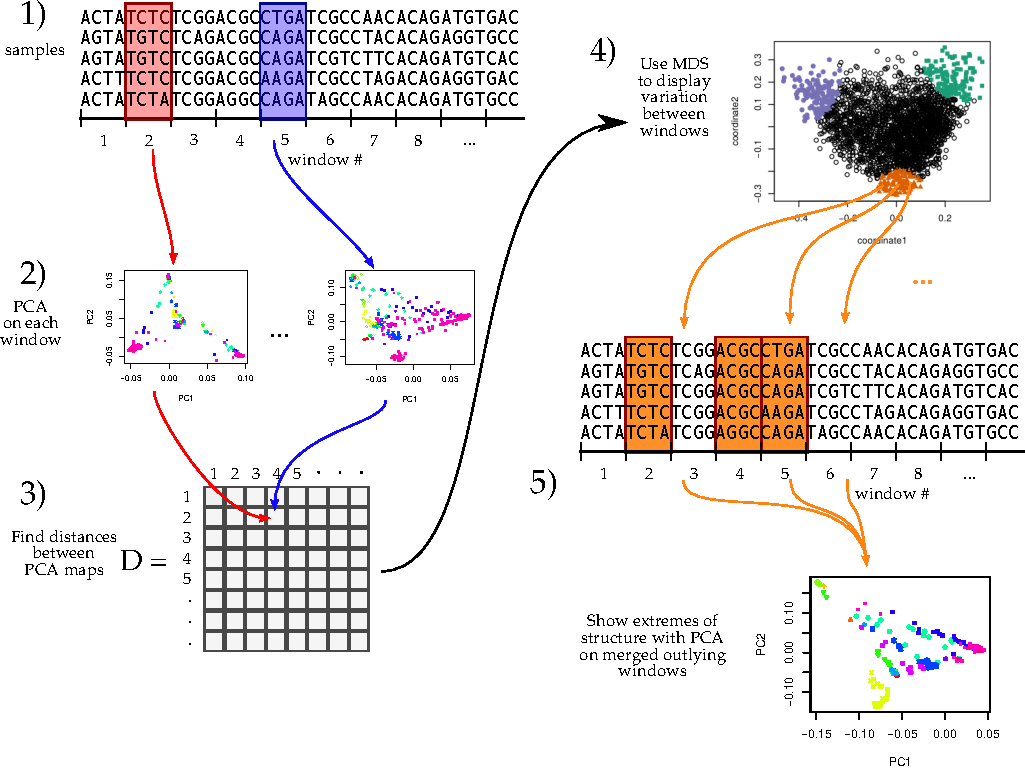
\includegraphics{the-method-diagram}
    \end{center}
    \caption{
         An illustration of the method; see Methods for details.
         % (1) the genome is divided into windows;
         % (2) population structure is summarized in each with PCA, and 
         % (3) dissimilarities for each are computed;
         % (4) the patterns of dissimilarity are visualized with MDS,
         % and (5) genomic regions clustering together are aggregated and visualized, again with PCA.
         \label{fig:diagram}
    }
\end{figure}



\subsection{PCA in genomic windows}

To begin,
we first recoded sampled genotypes as numeric matrices in the usual manner,
by recording the number of nonreference alleles seen at each locus for each sample.
We then divided the genome into contiguous segments 
(``windows'')
% recoded matrix into contiguous matrices that have the same columns but fewer rows than the original matrix, 
and applied principal component analysis (PCA) as described in \citet{mcvean2009genealogical}
separately to the submatrices that corresponded to each window.
The choice of window length entails a tradeoff between signal and noise,
since shorter windows allow better resolution along the genome but provide less precise estimates of relatedness.
A method for choosing a window length to balance these considerations is given in Appendix \ref{apx:window_length}.
% Specifically, we did PCA as follows:
Precisely,
denote by $Z$ the $L\times N$ recoded genotype matrix for a given window ($L$ is the number of SNPs and $N$ is the sample size), 
and by $\overline{Z_{s}}$ the mean of non-missing entries for allele $s$, 
so that $\overline{Z_{s}}=\frac{1}{n_s}\sum_j Z_{sj}$, 
where the sum is over the $n_s$ nonmissing genotypes.
We first compute the mean-centered matrix $X$, as $X_{si}=Z_{si}-\overline{Z_{s}}$,
and preserving missingness.
(This mean-centering makes the result not depend on the choice of reference allele,
exactly if there is no missing data, and approximately otherwise.)
Next, we find the covariance matrix of $X$, denoted $C$,
as $C_{ij} = \frac{1}{m_{ij}-1} \sum_s X_{si} X_{sj} - \frac{1}{m_{ij}(m_{ij}-1)} (\sum_s X_{si})(\sum_s X_{sj})$,
where all sums are over the $m_{ij}$ sites where both sample $i$ and sample $j$ have nonmissing genotypes.
% We compute the covariance matrix using the R function cov() , with use=``pairwise",
% which computes the covariance between each pair of individuals using all complete pairs of SNPs on those individuals.
The principal components are the eigenvectors of $C$, 
normalized to have Euclidean length equal to one,
and ordered by magnitude of the eigenvalues.

The top 2--5 principal components are generally good summaries of population structure; 
for ease of visualization we usually only use the first two (referred to as $\pcone$ and $\pctwo$),
and check that results hold using more. \revpoint{1}{6}
The above procedure can be performed on any subset of the data;
for future reference, denote by $\pcone_j$ and $\pctwo_j$
the result after applying to all SNPs in the $j^\text{th}$ window.
(Note, however, that our measure of dissimilarity between windows
does not depend on PC ordering.) \llabel{ll:another_pc_point}

% Several of the datasets we use have unbalanced representations of diverged populations,
% which can have a strong impact on the results of PCA.
% (The principal axes may describe variation \emph{within} an overrepresented group
% rather than more significant variation between groups.)
% Therefore, to check that sampling patterns do not affect our results,
% we compared to a variant of PCA that gives roughly equal weight to each group of samples,
% rather than to each sample.
% The rationale and implementation of this method are described in Appendix \ref{apx:weighted_pca}.


\subsection{Similarity of patterns of relatedness between windows}

We think of the local effects of population structure as being summarized by \emph{relative} position of the samples
in the space defined by the top principal components.
However, 
we do not compare patterns of relatedness of different genomic regions by directly comparing the PCs,
since rotations or reflections of these imply identical patterns of relatedness.
Instead, we compare the low-dimensional approximations of the local covariance matrices
obtained using the top $k$ PCs,
which is invariant under reordering of the PCs, \revpoint{1}{2}
reflections, and rotations and yet contains all other information about the PCs.
(For results shown here, we use $k=2$.)
Furthermore, to remove the effect of artifacts such as mutation rate variation,
we also rescale each approximate covariance matrix to be of similar size
(precisely, so that the underlying data matrix has trace norm equal to one).

To do this, define the $N \times k$ matrix $V(i)$ so that $V(i)_{\cdot \ell}$, 
the $\ell^\text{th}$ column of $V(i)$,
is equal to the $\ell^\text{th}$ principal component of the $i^\text{th}$ window,
multiplied by $( \lambda_{\ell i} / \sum_{m=1}^k \lambda_{m i} )^{1/2}$,
where $\lambda_{\ell i}$ is the $\ell^\text{th}$ eigenvalue of the genetic covariance matrix.
% \begin{equation}
%     \begin{aligned}
%         V_{i1}&=\sqrt{\frac{\lambda _{1i}}{\lambda _{1i}+\lambda _{2i}}}PC1_{i} ,
%         \qquad
%         V_{i2}&=\sqrt{\frac{\lambda _{2i}}{\lambda _{1i}+\lambda _{2i}}}PC2_{i} 
%     \end{aligned}
% \end{equation}
Then, the rescaled, rank $k$ approximate covariance matrix for the $i^\text{th}$ window is
\begin{align} \label{eqn:est_cov}
    M(i) &= \sum_{\ell=1}^k V(i)_{\cdot \ell} V(i)_{\cdot \ell}^T .
\end{align}
% \begin{align}
%     M_{i} &= \frac{\lambda_{1i}PC1_{i}PC1_{i}^{T}+\lambda_{2i}PC2_{i}PC2_{i}^{T}}{\lambda_{1i}+\lambda_{2i}} 
% \end{align}
To measure the similarity of patterns of relatedness for the $i^\text{th}$ window and $j^\text{th}$ window,
we then use
Euclidean distance $D_{ij}$ between the matrices $M(i)$ and $M(j)$,
defined by
$D_{ij}^2 = \sum_{k\ell} ( M(i)_{k,\ell} - M(j)_{k,\ell} )^2$.


The goal of comparing PC plots up to rotation and reflection 
turned out to be equivalent to comparing rank-$k$ approximations to local covariance matrices.
This suggests instead directly comparing entire local covariance matrices. 
However, with thousands of samples and tens of thousands of windows,
computing the distance matrix would take months of CPU time,
while as defined above, $D$ can be computed in minutes using the following method.
Since for square matrices $A$ and $B$,
$\sum_{ij} (A_{ij}-B_{ij})^2 = \sum_{ij} (A^2_{ij} + B^2_{ij}) - 2 \tr(A^T B)$,
then due to the orthogonality of eigenvectors and the cyclic invariance of trace,
$D_{ij}$ can be computed efficiently as
\begin{align}
    D_{ij} 
    = 
    \left(
    \frac{ \sum_{\ell=1}^k \lambda_{\ell i}^2 }{ (\sum_{\ell=1}^k \lambda_{\ell i})^2 }
    + \frac{ \sum_{\ell=1}^k \lambda_{\ell j}^2 }{ (\sum_{\ell=1}^k \lambda_{\ell j})^2 }
    - 2 \sum_{\ell, m=1}^k (V(i)^T V(j))^2_{\ell m} 
    \right)^{1/2}.
\end{align}
% from the code for pc_dist():
% #' In the unweighted case, suppose that (u) and (v) are sets of vectors, and that 
% #'    A = a_1 * u_1 u_1^T + ... + a_j * u_j u_j^T = U diag(a) U^T
% #'    B = b_1 * v_1 v_1^T + ... + b_j * v_k v_k^T = V diag(b) V^T,
% #' where U is the matrix whose columns are (u), and likewise for V.
% #' Then 
% #'    (A-B)^T (A-B) = A^T A + B^T B - A^T B - B^T A
% #' and so
% #'    ||A-B||^2 = ||A||^2 + ||B||^2 - 2 tr( A^T B )
% #' By the cyclic invariance of trace, if X = U^T V then
% #'    tr( A^T B ) = tr( U diag(a) U^T V diag(b) V^T ) = tr( diag(a) X diag(b) X^T ) .
% \begin{align}
%     \begin{split}
%     D_{ij} &= 
%         \left \{
%                 \left ( 
%                     V_{i1}\cdot V_{i1}^{} 
%                 \right )^{2}
%                 + \left ( V_{i2}\cdot V_{i2}^{} \right )^{2}
%                 + \left ( V_{j1}\cdot V_{j1}^{} \right )^{2} 
%                 +\left ( V_{j2}\cdot V_{j2}^{} \right )^{2} 
%         \right. \\ 
%         & \left. \qquad {}  
%             -2\left [ 
%                 \left ( V_{i1}\cdot V_{j1}^{} \right )^{2}
%                 + \left ( V_{i1}\cdot V_{j2}^{} \right )^{2}
%                 + \left ( V_{i2}\cdot V_{j1}^{} \right )^{2} 
%                 + \left ( V_{i2}\cdot V_{j2}^{} \right )^{2}
%             \right ]
%         \right \}^{1/2}
%     \end{split}
% \end{align}

%%%%%%%%%%%%%%%%%%%%%%%%%%%%%%%%%%%%%
\subsection{Visualization of results}

We use multidimensional scaling (MDS) to visualize relationships between windows
as summarized by the dissimilarity matrix $D$.
MDS produces a set of $m$ coordinates for each window that
give the arrangement in $m$-dimensional space that best recapitulates the original distance matrix.
For results here, we use $m=2$ to produce one- or two-dimensional visualizations of relationships between windows' patterns of relatedness.

We then locate variation in patterns of relatedness along the genome
by choosing collections of windows that are nearby in MDS coordinates,
and map their positions along the genome.
A visualization of the effects of population structure across the entire collection is formed by extracting the corresponding genomic regions
and performing PCA on all, aggregated, regions.

%%%%%%%%%%%%%%%%%%%
\subsection{Testing}
\label{ss:testing_methods}

We tested the method using two types of simulation.
First, to verify expected behavior, we simulated ``genomes'' as an independent sequence
of correlated Gaussian ``genotypes'', using a different covariance matrix
in the first quarter, middle half, and last quarter of the chromosome.
The details of the simulation,
also designed to detect sensitivity to PC switching,
are given in Appendix \ref{apx:gaussian_sims}.
To verify robustness to missing data,
we ran the method after randomly dropping 50\% of the genotypes in the first half of the genome;
if the method is misled by missing data, then it will distinguish the two halves of the chromosome
rather than the segments having different covariance matrices.

To provide a realistic test,
we next used forwards-time, individual-based simulations, implemented using SLiM v3 \citep{haller2017flexible},
which are described in detail in Appendix \ref{apx:slim_sims}.
To provide realistic population structure for PCA to identify,
each simulation had at least 5,000 diploid individuals,   
living across a continuous square range,
with Gaussian dispersal and local density-dependent competition.
Each genome was modeled on human chromosome 7, which is $1.54 \times 10^8$bp long,
with an overall recombination rate of 1.6785 crossovers per chromosome per generation.
To improve speed, we used tskit \citep{kelleher2018efficient} to record tree sequences 
in SLiM \citep{haller2018treesequence}
and to add neutral mutations afterwards, at a rate of $10^{-9}$ per bp per generation.
Most simulations were neutral, but we also included linked selection, of two types.
First, % run_031486
we introduced selected mutations into two regions, 
which extended from 1/3 to 1/2 and from 5/6 to the end of the genome respectively.
These had selection coefficients from a Gamma distribution with shape 2 and mean 0.005
at a rate of $10^{-10}$ per bp, that were either beneficial (with probability $1/30$)
or deleterious (otherwise).
Second, % run_016913
to roughly model a recent expansion followed by local adaptation,
we introduced mutations in the same manner as above,
except that mutations were no longer unconditionally deleterious or beneficial:
each selection coefficient was multiplied by a factor depending on the spatial location
of the individual being evaluated, varying linearly from -1 at the left side of the range
to +1 at the right edge.
In all simulations, genome-wide PCA displayed a map of the population range, as expected.


\subsection{Datasets}
% Recode the DNA sequence to a matrix consisting of 0,1,2 (and NA).

We applied the method to genomic datasets with good geographic sampling:
380 African \textit{Drosophila melanogaster} from the Drosophila Genome Nexus \citep{lack2015drosophila},
a worldwide dataset of humans,
3,965 humans from several locations worldwide from the POPRES dataset \citep{nelson2008population},
and 263 \textit{Medicago truncatula} from 24 countries around the Mediterranean basin 
a range-wide dataset of the partially selfing weedy annual plant 
from the \textit{Medicago truncatula} Hapmap Project \citep{tang2014improved},
as summarized in Table \ref{tab:data_stats}.

\paragraph{\textit{Drosophila melanogaster}:}
We used whole-genome sequencing data 
from the Drosophila Genome Nexus (\url{http://www.johnpool.net/genomes.html}, \citep{lack2015drosophila}),
consisting of the Drosophila Population Genomics Project phases 1--3 \citep{langley2012genomic,pool2012population},
and additional African genomes \citep{lack2015drosophila}.
After removing 20 genomes with more than 8\% missing data,
we were left with 380 samples from 16 countries across Africa and Europe.
Since the \textit{Drosophila} samples are from inbred lines or haploid embryos, 
we treat the samples as haploid when recoding;
regions with residual heterozygosity were marked as missing in the original dataset;
we also removed positions with more than 20\% missing data. 
% (We chose these cutoffs as the tails of the relevant empirical distributions.)
Each chromosome arm we investigated (X, 2L, 2R, 3L, and 3R) has 2--3 million SNPs;
PCA plots for each arm are shown in \Figure \ref{sfig:pca_drosophila_allchr}.

\paragraph{Human:}
We also used genomic data from the entire POPRES dataset \citep{nelson2008population},
which has array-derived genotype information for 447,267 SNPs across the 22 autosomes
of 3,965 samples in total: 346 African-Americans, 73 Asians, 3,187 Europeans and 359 Indian Asians.
Since these data derive from genotyping arrays, the SNP density is much lower than the other datasets,
which are each derived from whole genome sequencing.
We excluded the sex chromosomes and the mitochondria.
PCA plots for each chromosome, separately, are shown in \Figure \ref{sfig:pca_human_allchr}.
% We use the allele that has highest frequency in the samples as the reference allele for each position. 

% lack2015drosophila: describes the DGN, including the AGES samples.  reports diversity and mentions inversions but mostly a 'data' paper
% pool2012population: describes 129 subsaharan samples (DPGP3)

\paragraph{\textit{Medicago truncatula}:}
Finally, we used whole-genome sequencing data from the \textit{Medicago truncatula} Hapmap Project \citep{tang2014improved},
which has 263 samples from 24 countries,
primarily distributed around the Mediterranean basin.
Each of the 8 chromosomes has 3--5 million SNPs;
PCA plots for these are shown in \Figure \ref{sfig:pca_medicago_allchr}.
We did not use the mitochondria or chloroplasts.

\begin{table}[ht]
\centering
    \begin{tabular}{p{0.8in}rrrr}
  \hline
    species 
    & \parbox[t]{.8in}{\# SNPs per \\ window} 
    & \parbox[t]{1in}{mean window\\ length (bp)}
    & \parbox[t]{1.2in}{mean \# windows \\ per chromosome} 
    & \parbox[t]{1.4in}{mean \% variance ex-\\plained by top 2 PCs} \\ 
  \hline
  \textit{Drosophila melanogaster} & 1,000 & 9,019 & 2,674 & 0.53 \\ 
  Human & 100 & 636,494 & 203 & 0.55 \\ 
  \textit{Medicago truncatula} & 10,000 & 102,580 & 467 & 0.50 \\ 
   \hline
\end{tabular}
\caption{
    Descriptive statistics for each dataset used.
    % \revpoint{2}{18}  %% no line numbers here; won't work
    % % with the chosen window sizes.
    % % See text for how window sizes were chosen;
    % Columns 2--4 give statistics describing the window sizes used for most analyses for each dataset
    % (windows had a fixed number of SNPs).
    % The final column gives the percent variance explained by the top two principal components,
    % averaged across independent PCA of each window.
    \label{tab:data_stats}
}
\end{table}

\subsection{Data access}

The methods described here
are implemented in an open-source R package
available at \url{https://github.com/petrelharp/local_pca},
as well as scripts to perform all analyses from VCF files
at various parameter settings.

Datasets are available as follows:
human (POPRES) at dbGaP with accession number phs000145.v4.p2,
\textit{Medicago} at the Medicago Hapmap \url{http://www.medicagohapmap.org/},
and \textit{Drosophila} at the Drosophila Genome Nexus, \url{http://www.johnpool.net/genomes.html}.


%%%%%%%%%%%%%%%%%%%%%%%%%%%%%%
\section{Results}

In all three datasets:
a worldwide sample of humans, African \textit{Drosophila melanogaster},
and a rangewide sample of \textit{Medicago truncatula},
PCA plots vary along the genome in a systematic way, showing strong chromosome-scale correlations.
This implies that variation is due to meaningful heterogeneity in a biological process,
since noise due to randomness in choice of local genealogical trees
is not expected to show long distance correlations. 
Below, we discuss the results and likely underlying causes.




%%%%%%%%%%%
\subsection{Validation}
\label{ss:validation}

Simple non-population-based simulations with Gaussian ``genotypes''
showed that the method performs as expected, clearly separating regions of the genome
with different underlying covariance matrices
without being affected by extreme differences in amount of missing data
(Supplemental Figure \ref{sfig:test_missing}).
This simulation also verifies insensitivity to ordering of top PCs,
since it was performed using a covariance matrix with the top two eigenvalues equal,  
so that the order of empirical eigenvectors (PCs) switches randomly.

Individual-based simulations using SLiM \citep{haller2017flexible} allowed us to test the effects
of recombination and mutation rate variation, as well as linked selection.
As expected, varying recombination rate stepwise by a factor of 64
did not induce patterns in the MDS visualizations correlated with recombination rate
(Supplemental Figure \ref{sfig:slim_sims1}).
\llabel{ll:test_recomb_rate}
Since varying mutation rate with a fixed recombination map
is equivalent to varying the recombination map and remapping windows,
this also indicates that the method is not misled by variation in mutation rate.
On the other hand,
a recombination map with hotspots
(the HapMap human female map for chromosome 7 \citep{hapmap2007second})
induced outliers at long regions of low recombination rate
(also as expected). \llabel{ll:hotspot_recomb}

Simulations with linked selection produced mixed results
(Figure \ref{sfig:slim_sims2}).
The method strongly identified the regions under spatially varying linked selection.
It also identified the regions (although less unambiguously)
with constant selection and stepwise varying recombination rate,
but did not clearly identify them with constant recombination rate.
This difference is likely because recombination rates are overall lower in the first case,
leading to a stronger effect of linked selection.
These tests are not meant to be comprehensive survey of linked selection,
but only to demonstrate that linked selection can produce signals similar to what we see in real data.


%%%%%%%%%%%
\subsection{\textit{Drosophila melanogaster}}

We applied the method to windows of average length 9 Kbp, across chromosome arms 2L, 2R, 3L, 3R and X separately.
The first column of \Figure \ref{fig:mds_allchr} is a multidimensional scaling (MDS) visualization 
of the matrix of dissimilarities between genomic windows:
in other words, genomic windows that are closer to each other in the MDS plot show more similar patterns of relatedness.
For each chromosome arm, the MDS visualization roughly resembles a triangle,
sometimes with additional points.
Since the relative position of each window in this plot shows the similarity between windows, 
this suggests that there are at least three extreme manifestations of population structure 
typified by windows found in the ``corners'' of the figure,
and that other windows' patterns of relatedness may be a mixture of those extremes. 
The next two columns of \Figure \ref{fig:mds_allchr} respectively depict the two MDS coordinates of each window,
plotted against the window's position along the genome,
to show how the plot of the first column is laid out along the genome.
The patterns did not depend on the number of PCs used
(see \Figure \ref{sfig:dmel_k5} for the same plot with $k=5$ PCs), \revpoint{1}{3}
and are only weakly correlated with variation in missingness 
(see \Figure \ref{sfig:dpgp_missingness}). \revpoint{2}{4}


\begin{figure}
    \begin{center}
        \ifusepngs
           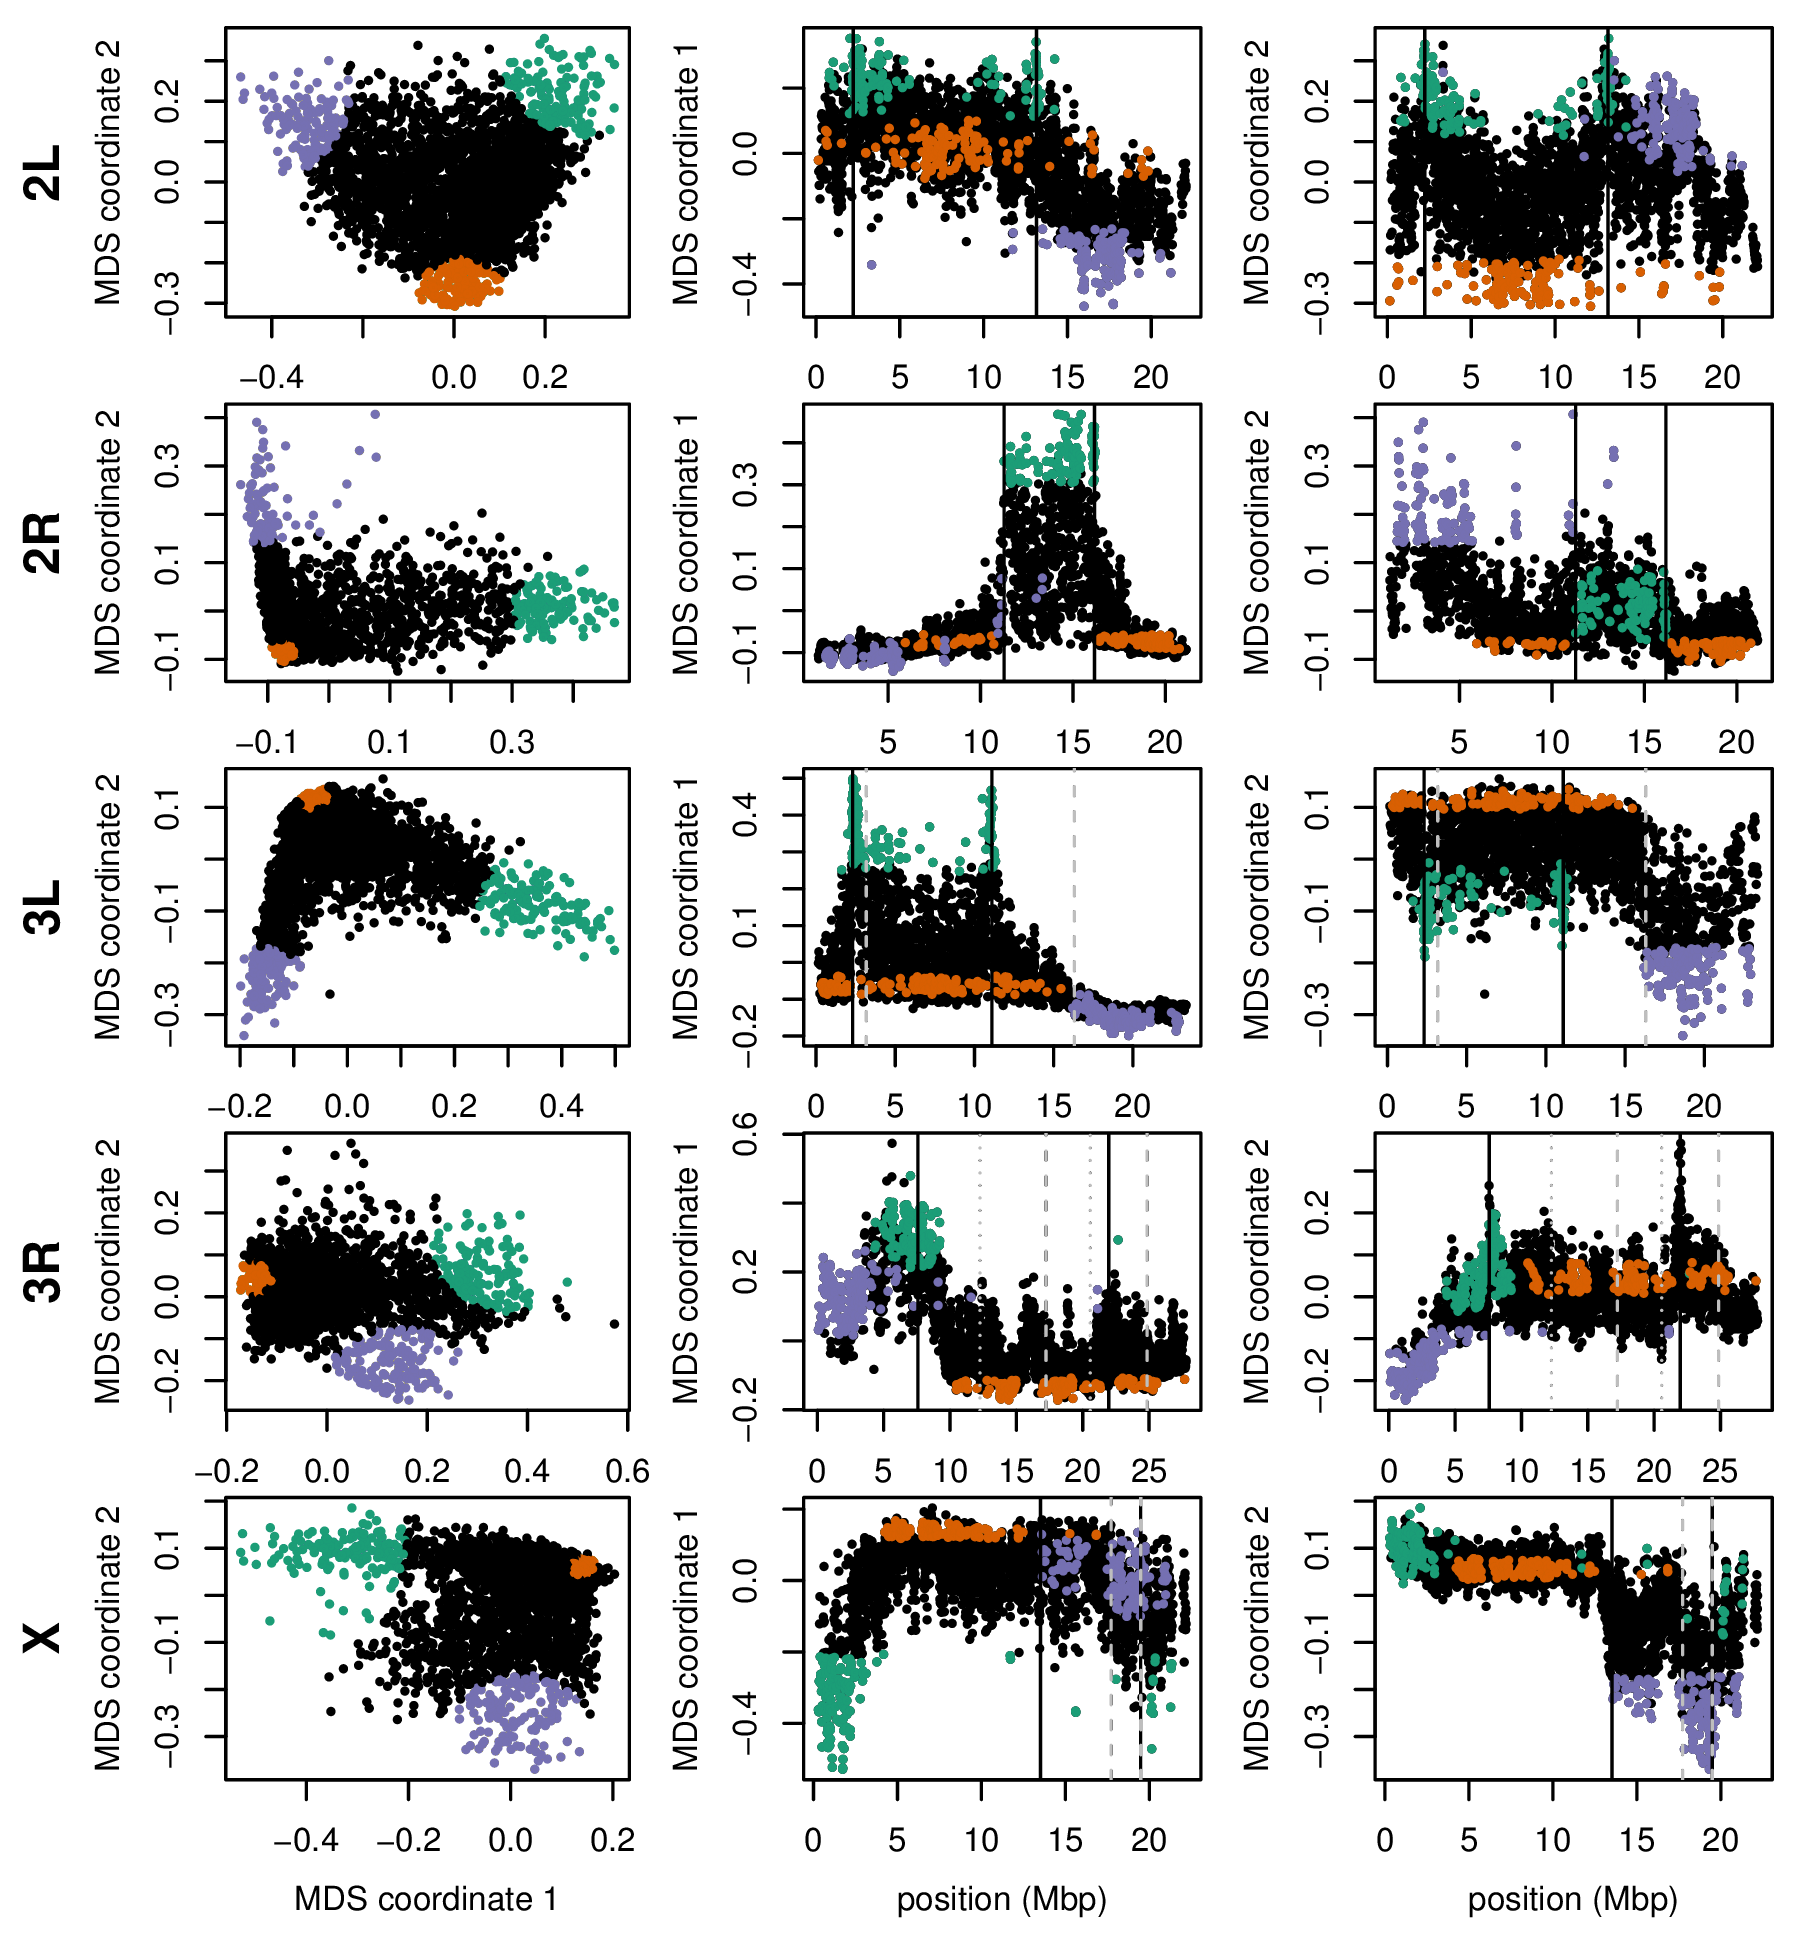
\includegraphics[width=0.9\textwidth]{Fig1_allchr_Together_MDS_plot_compact_with_ChrX_inv.png}
       \else
           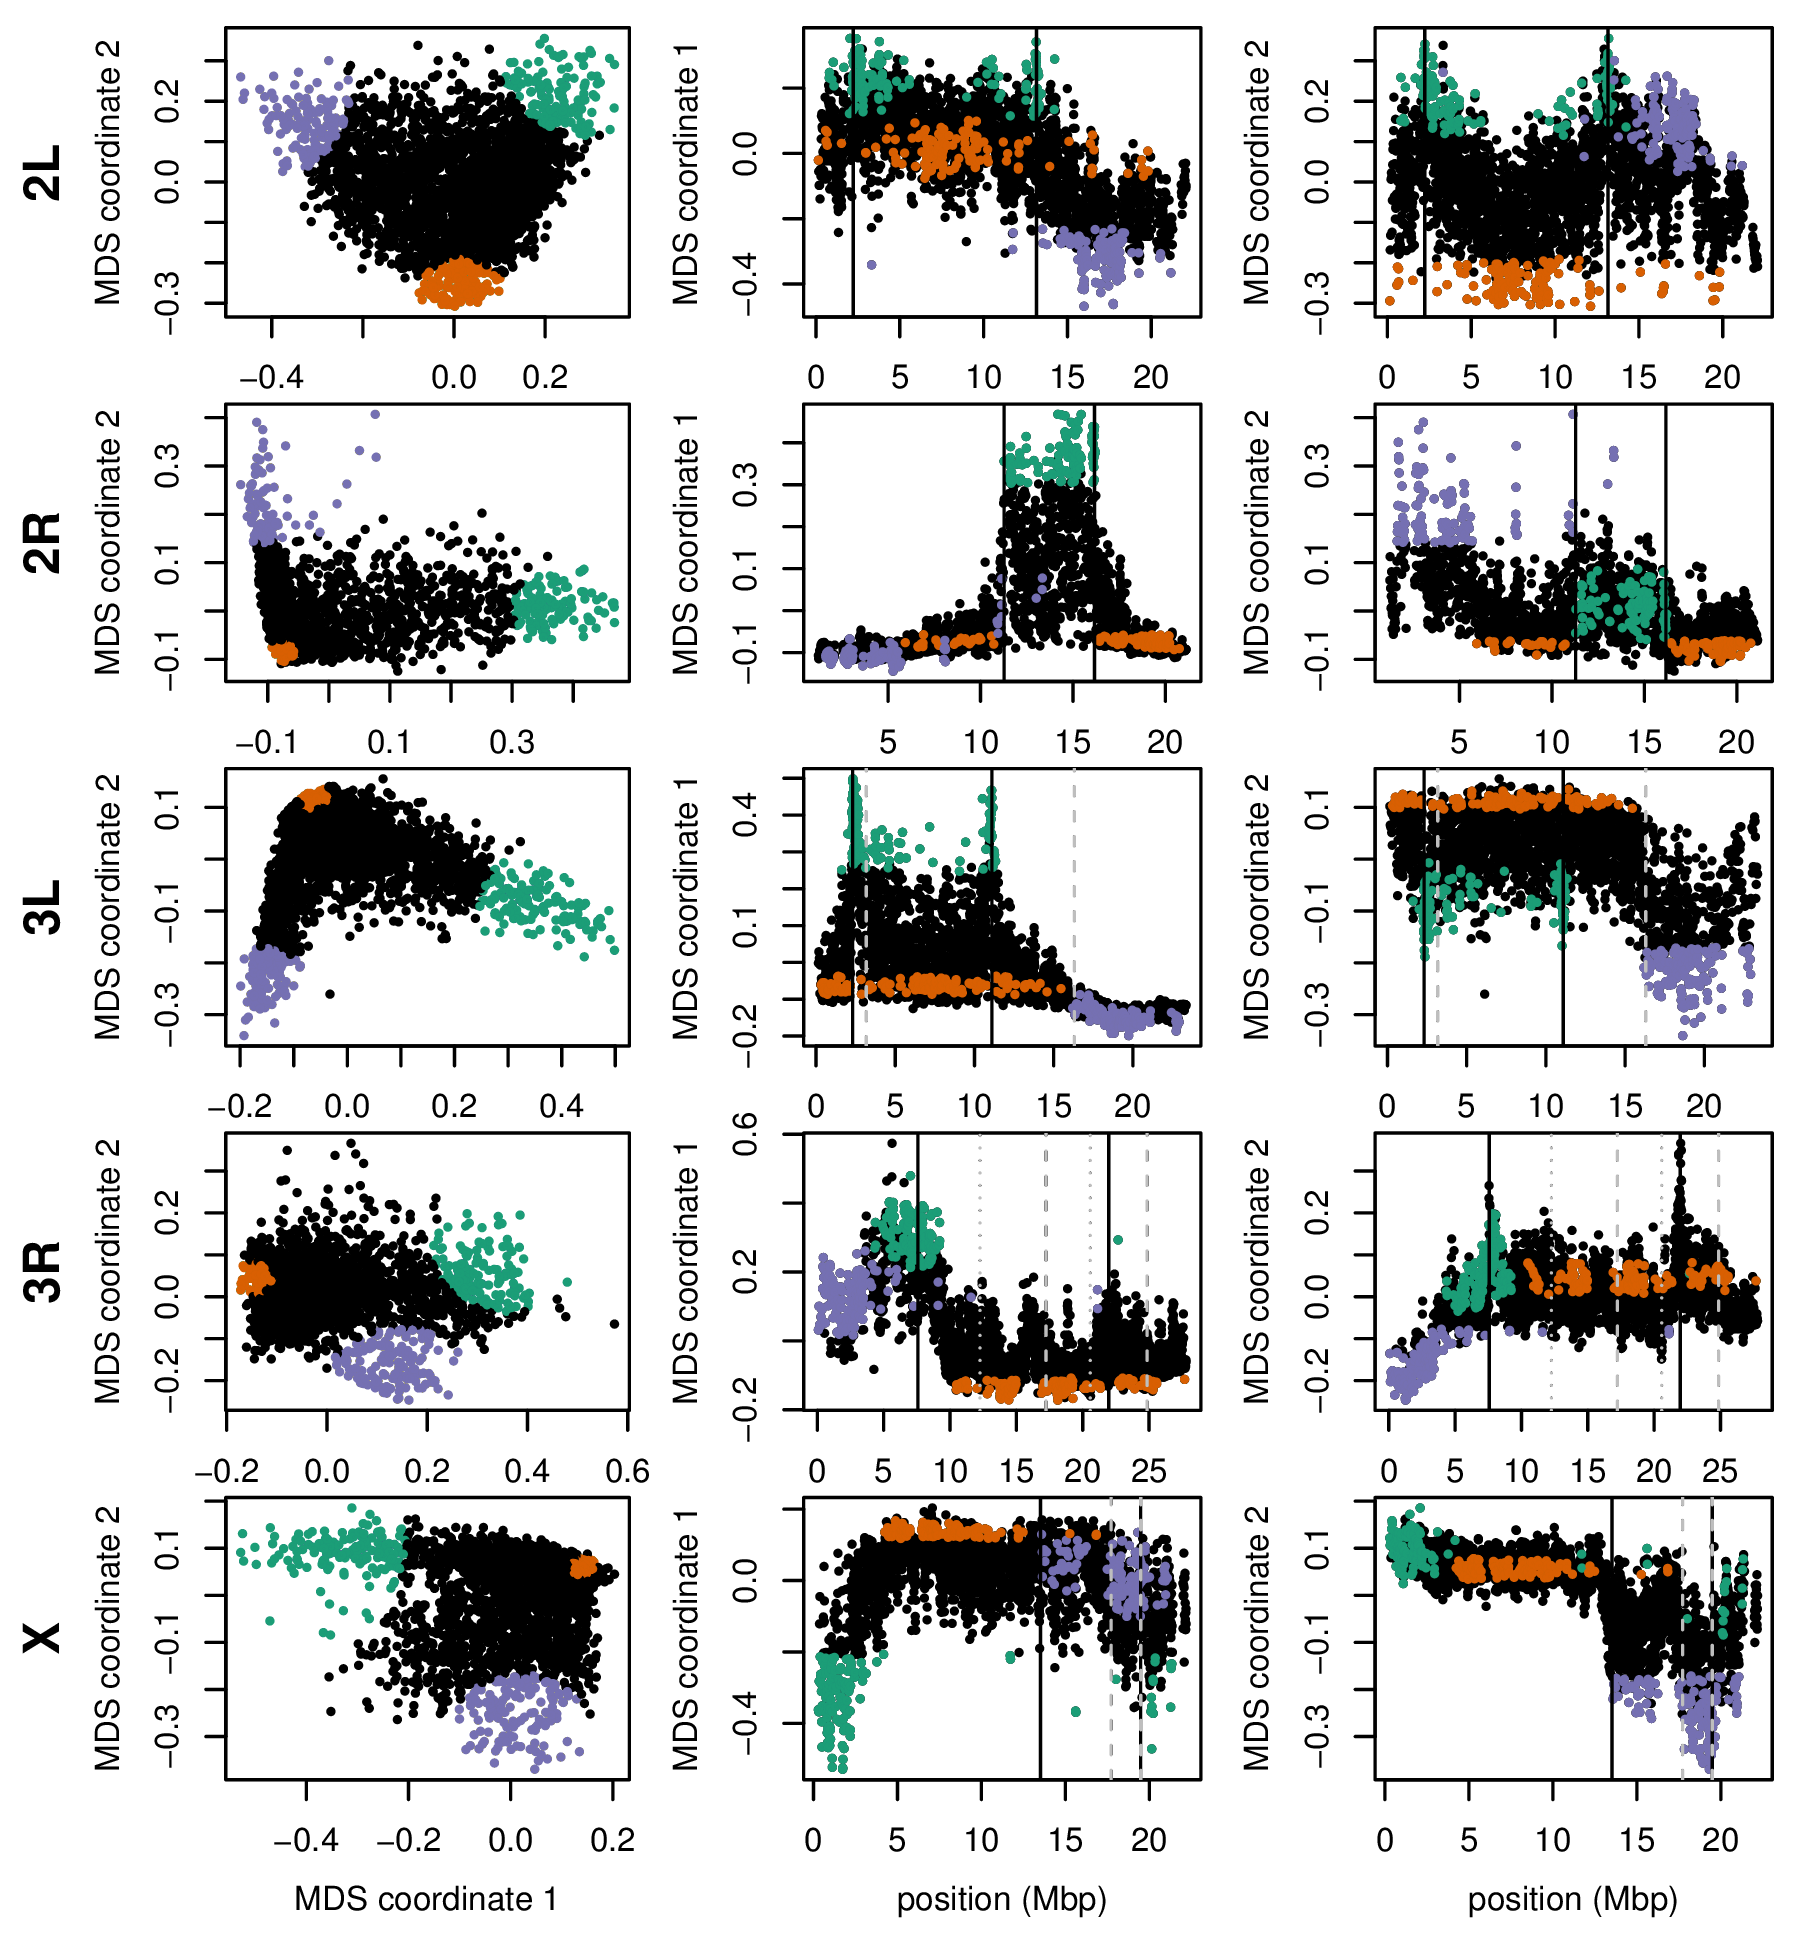
\includegraphics[width=0.9\textwidth]{Fig1_allchr_Together_MDS_plot_compact_with_ChrX_inv}
       \fi
    \end{center}
    \caption{
        Variation in patterns of relatedness for windows across \textit{Drosophila melanogaster} chromosome arms.
        In all plots, each point represents one window along the genome.
         The first column shows the MDS visualization of relationships between windows, 
         and the second and third columns show 
        the two MDS coordinates
         against the midpoint of each window;
         rows correspond to chromosome arms.
         Colors are consistent for plots in each row. 
         Vertical lines show the breakpoints of known polymorphic inversions.   
         Solid black lines are for the inversions we used in \Figure \ref{fig:pca_by_inversion},
         while dotted grey lines are for other known inversions.     
         \label{fig:mds_allchr}
    }
\end{figure}



To help visualize how clustered windows with similar patterns of relatedness are along each chromosome arm, 
we selected three ``extreme'' windows in the MDS plot
and the 5\% of windows that are closest to it in the MDS coordinates,
then highlighted these windows' positions along the genome,
and created PCA plots for the windows, combined.
Representative plots are shown for three groups of windows on each chromosome arm
in \Figure \ref{fig:mds_allchr} (groups are shown in color),
and in Supplemental \Figure \ref{sfig:pca_by_pop} (PCA plots).
The latter plots are quite different,
showing that genomic windows in different regions of the MDS plot 
indeed show quite different patterns of relatedness.


The most striking variation in patterns of relatedness turns out to be explained by
several large inversions that are polymorphic in these samples, 
discussed in \citet{corbett2012population} and \citet{langley2012genomic}.
% Frequencies of each inversion in the sample are given in Table \ref{tab:inversion_freqs}.
To depict this, \Figure \ref{fig:pca_by_inversion} shows
the PCA plots in Supplemental \Figure \ref{sfig:pca_by_pop} recolored by the orientation of the inversion for each sample.
Taking chromosome arm 2L as an example,
the two regions of similar, extreme patterns of relatedness
shown in green in the first row of \Figure \ref{fig:mds_allchr}
lie directly around the breakpoints of the inversion In(2L)t,
and the PCA plots in the first rows of \Figure \ref{fig:pca_by_inversion}
shows that patterns of relatedness here are mostly determined by inversion orientation.
The regions shown in purple on chromosome 2L lie near the centromere,
and have patterns of relatedness reflective of two axes of variation,
seen in \Figure \ref{fig:pca_by_inversion} and Supplemental \Figure \ref{sfig:pca_by_pop},
which correspond roughly to latitude within Africa and to degree of cosmopolitan admixture respectively
(see \citet{lack2015drosophila} for more about admixture in this sample).
The regions shown in orange on chromosome 2L mostly lie inside the inversion,
and show patterns of relatedness that are a mixture between the other two,
as expected due to recombination within the (long) inversion \citep{guerrero2011coalescent}.
Similar results are found in other chromosome arms,
albeit complicated by the coexistence of more than one polymorphic inversion;
however, each breakpoint visibly affects patterns in the MDS coordinates
(see vertical lines in \Figure \ref{fig:mds_allchr}).

% \plr{\citet{corbett2012population} says In(1)Be is very young, $\sim$ 60 years.
% Also cite \citet{corbettdetig2012sequencebased} for a computational method for detecting inversions.}
% corbettdetig2012sequencebased suggests these inversions are recent-ish (but before out-of-Africa)
% except that the situation of Chr3R is a little more complicated,
% due to the coexistence of two polymorphic inversions (In(3R)K and In(3R)P) at intermediate frequency.
% However, peaks in MDS coordinates along the chromosome show the breakpoints of both,
% although we have not highlighted portions of the MDS plot that pick these out.
% The inversions In(3L)P and In(3R)Mo, are at low frequency in these samples, 
% and visibly affect the MDS plots although less than the more common inversion on each arm.
% The very young inversion In(X)be shows little signal 
% compared to the older inversion In(X)A \citep{corbett2012population}.

\begin{figure}
    \begin{center}
       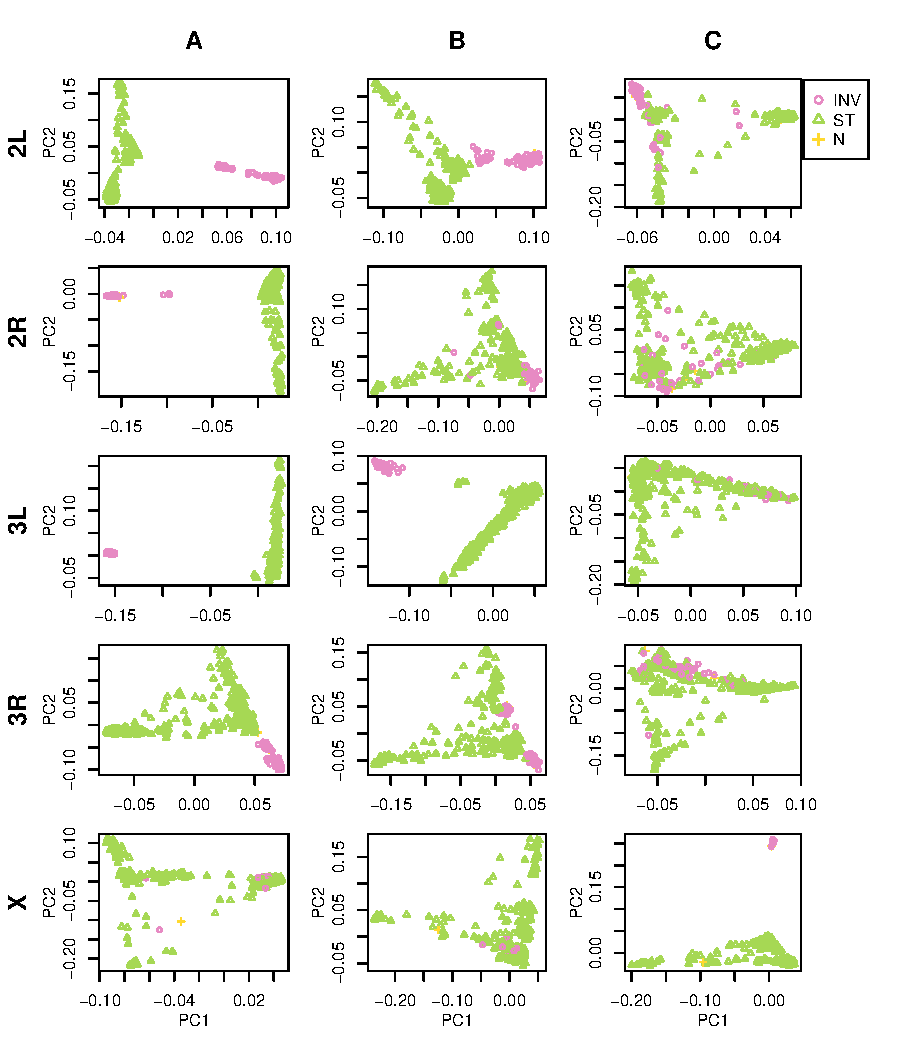
\includegraphics{Fig3_pca_plots_color_by_inv_allchr_with_ChrX_In1A}
    \end{center}
    \caption{
        PCA plots for the three sets of genomic windows colored in \Figure \ref{fig:mds_allchr},
        on each chromosome arm of \textit{Drosophila melanogaster}.
        In all plots, each point represents a sample. 
        The first column shows the combined PCA plot for windows 
        whose points are colored green in \Figure \ref{fig:mds_allchr}; 
        the second is for orange windows; 
        and third is for purple windows.
         In each, samples are colored by orientation of the polymorphic inversions 
         In(2L)t, In(2R)NS, In(3L)OK, In(3R)K and In(1)A respectively
         (data from \citep{lack2015drosophila}).
         In each ``INV'' denotes an inverted genotype, ``ST'' denotes the standard orientation,
         and ``N'' denotes unknown.
        \label{fig:pca_by_inversion}
    }
\end{figure}

To see how patterns of relatedness vary in the absence of polymorphic inversions,
we performed the same analyses after removing, for each chromosome arm,
any samples carrying inversions on that arm.
In the result, shown in \Figure \ref{fig:drosophila_recomb_rate} and
Supplemental \Figure \ref{sfig:mds_allchr_noinversions},
the striking peaks associated with inversion breakpoints are gone,
and previously smaller-scale variation now dominates the MDS visualization.
For instance, the majority of the variation along 3L in \Figure \ref{fig:mds_allchr}
is on the left end of the arm, dominated by two large peaks around the inversion breakpoints;
there is also a relatively small dip on the right end of the arm (near the centromere).
In contrast, Supplemental \Figure \ref{sfig:mds_allchr_noinversions} shows that after removing polymorphic inversions,
remaining structure is dominated by the dip near the centromere.
Without inversions, variation in patterns of relatedness shown in the MDS plots
follows similar patterns to that previously seen in \textit{D.~melanogaster} recombination rate and diversity \citep{langley2012genomic,mackay2012drosophila}.
Indeed, correlations between the recombination rate in each window and the position on the first MDS coordinate are highly significant
(Spearman's $\rho=0.54$, $p<2 \times 10^{-16}$; \Figures \ref{fig:drosophila_recomb_rate} and \ref{sfig:drosophila_gene_density_correlations}).
This is consistent with the hypothesis that variation
is due to selection, since the strength of linked selection increases with local gene density, 
measured in units of recombination distance.
The number of genes -- measured as the number of transcription start and end sites within each window --
was not significantly correlated with MDS coordinate ($p=0.22$).


\begin{figure}
    \begin{center}
        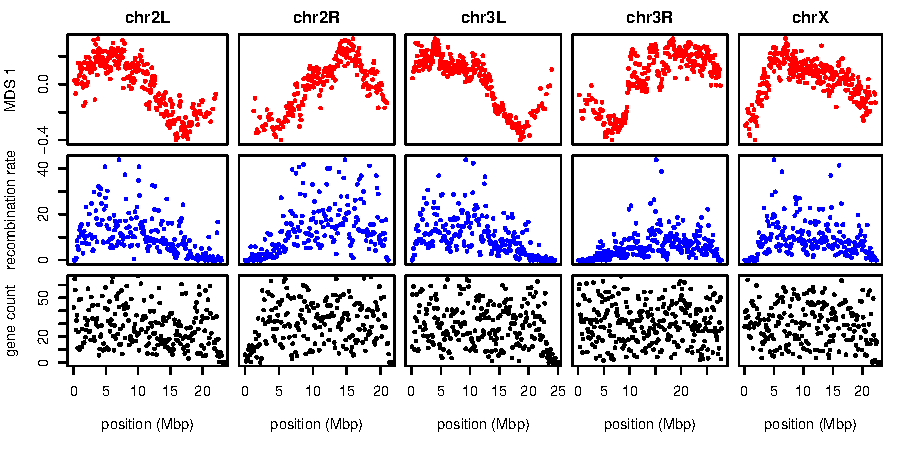
\includegraphics{drosophila_recomb_mds}
    \end{center}
    \caption{
        The effects of population structure without inversions is correlated to recombination rate in \textit{Drosophila melanogaster}.
        The first plot (in red) shows the first MDS coordinate along the genome 
        for windows of 10,000 SNPs,
        obtained after removing samples with inversions.
        (A plot analogous to \Figure \ref{fig:mds_allchr} is shown
        in Supplemental \Figure \ref{sfig:mds_allchr_noinversions}.)
        The second plot (in blue) shows
        local average recombination rates in cM/Mbp, obtained as midpoint estimates for 100Kbp windows 
        from the Drosophila recombination rate calculator \citep{fistonlavier2010drosophila} release 5,
        using rates from \citet{comeron2012many}.
        The third plot (in black) shows the number of genes' transcription start and end sites within each 100Kbp window, divided by two.
        Transcription start and end sites were obtained from the RefGene table from the UCSC browser. %, assembly dm3, on August 11, 2016.
        The histone gene cluster on chromosome arm 2L is excluded.
        \label{fig:drosophila_recomb_rate}
    }
\end{figure}


%%%%%%%%%%%
\subsection{Human}

As we did for the \textit{Drosophila} data, we applied our method separately to all 22 human autosomes.
On each, variation in patterns of relatedness was dominated by a small number of windows
having similar patterns of relatedness to each other that differed dramatically from the rest of the chromosome.
These may be primarily inversions: outlying windows coincide with
three of the six large polymorphic inversions described in \citet{antonacci2009characterization},
notably a particularly large, polymorphic inversion on 8p23 (\Figure \ref{fig:mds_human}). 
% for instance, the eleven windows that are outliers in the first MDS coordinate of chromosome 8 (\Figure \ref{fig:mds_human}) 
Similar plots for all chromosomes are shown
in Supplementary \Figures \ref{sfig:mds12_chr1_8_human}, \ref{sfig:mds12_chr9_16_human}, and \ref{sfig:mds12_chr17_22_human}.
PCA plots of many outlying windows show a characteristic trimodal shape 
(shown for chromosome 8 in \Figure \ref{sfig:pca_chr8_outliers}),
presumably distinguishing samples having each of the three diploid genotypes for each inversion orientation
(although we do not have data on orientation status).
This trimodal shape has been proposed as a method to identify inversions \citep{ma2012investigation},
but distinguishing this hypothesis from others,
such as regions of low recombination rate,
would require additional data.

We also applied the method on all 22 autosomes together, 
and found that, remarkably, 
the inversion on chromosome 8 is still the most striking outlying signal (\Figure \ref{sfig:mds1_along_allchr_human}). 
Further investigation with a denser set of SNPs,
allowing a finer genomic resolution,
may yield other patterns.

\begin{figure}
    \begin{center}
       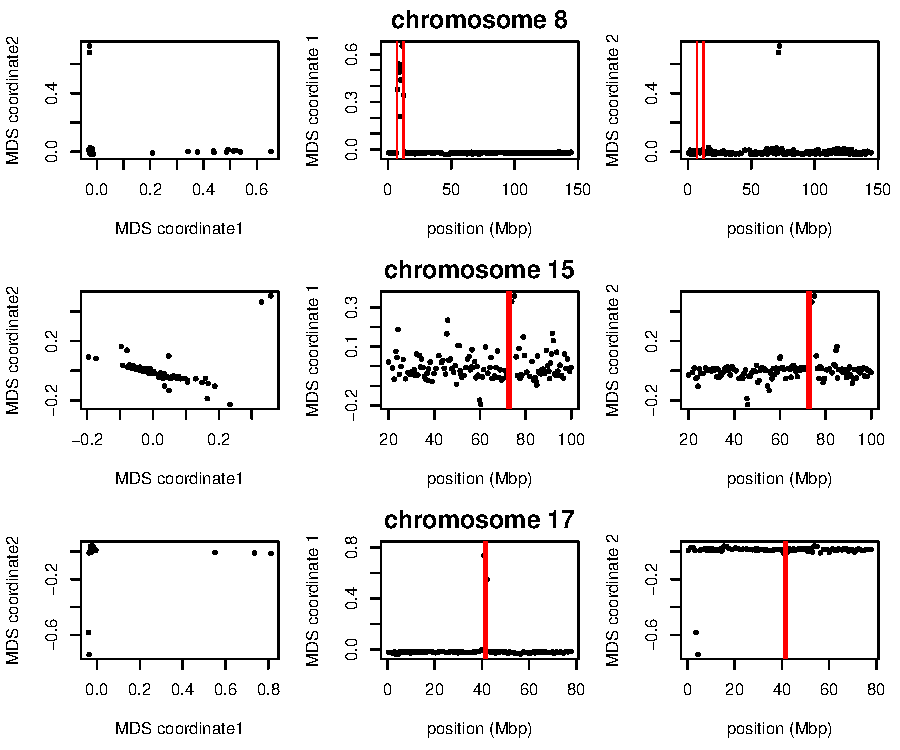
\includegraphics[width=0.9\textwidth]{Fig4_POPRES_Together_MDS_plot_chr8_15_17}
    \end{center}
    \caption{
         Variation in structure between windows on human chromosomes 8, 15, and 17. 
         Each point in each plot represents a window.
         The first column shows the MDS visualization of relationships between windows;
         the second and third columns show the two MDS coordinates of each window against its position (midpoint) along the chromosome. 
         Rows, from top to bottom show chromosomes 8, 15, and 17. 
         The vertical red lines show the breakpoints of known inversions from \citet{antonacci2009characterization}.
        \label{fig:mds_human}
    }
\end{figure}


%%%%%%%%%%%
\subsection{\textit{Medicago truncatula}}


Unlike the other two species,
the method applied separately on all eight chromosomes of \textit{Medicago truncatula} 
showed similar patterns of gradual change in patterns of relatedness across each chromosome,
with no indications of chromosome-specific patterns.
This consistency suggests that the factor affecting the population structure for each chromosome is the same,
as might be caused by varying strengths of linked selection.
To verify that variation in the effects of population structure is shared across chromosomes,
we applied the method to all chromosomes together.
Results for chromosome 3 are shown in \Figure \ref{fig:mds12_medicago}, \revpoint{2}{13}
and other chromosomes are similar:
across chromosomes, the high values of the first MDS coordinate coincide with the position of the heterochromatic regions surrounding the centromere,
which often have lower gene density and may therefore be less subject to linked selection.
% Selection on genes in Medicago has been demonstrated by \citet{paape2013selection}. 
To verify that this is a possible explanation,
we counted the number of genes found in each window using gene models in Mt4.0 from \url{jcvi.org} \citep{tang2014improved},
which are shown juxtaposed with
the first MDS coordinate of each window in \Figure \ref{fig:mds_medicago},
and are significantly correlated, as shown in Supplemental \Figure \ref{sfig:mds_gene_count}.
(Values shown are the number of start and end positions of each predicted mRNA transcript,
divided by two, assigned to the nearest window.)
% that lie closer to SNPs  between the last SNP of each window and the first SNP in the next window.
However, other genomic features, such as distance to centromere show roughly the same patterns,
so we cannot rule out alternative hypotheses.
In particular, fine-scale recombination rate estimates are not available in a form mappable
to Mt4.0 coordinates (although those in \citet{paape2012finescale} appear visually similar).
\revpoint{2}{8}

The results were highly consistent across window sizes, window types (SNPs or bp),
and number of PCs, as shown in Table \ref{tab:param_cors}.
\revpoint{1}{4} \revpoint{1}{5}
% We also found nearly identical results when choosing shorter windows of 1,000 SNPs
% (Supplemental Figure \ref{sfig:mds_medicago_allchr_1e3}; \revpoint{1}{4}
% or choosing windows of equal length in base pairs rather than SNPs. \revpoint{1}{5}
% Similarly, the results were not substantially changed
% when using weighted PCA to downweight the large group of Tunisian samples.

\begin{figure}
    \begin{center}
       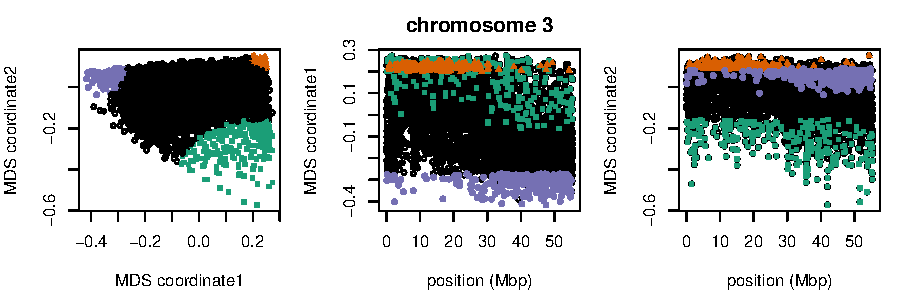
\includegraphics{Fig6_Together_MDS_plot_chr3_final}
       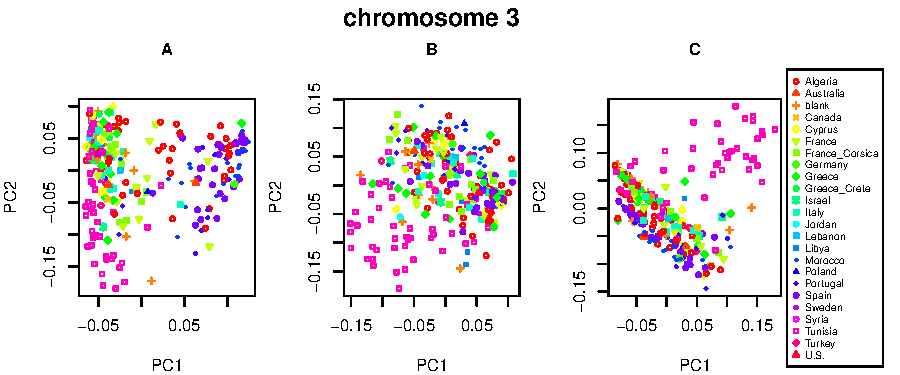
\includegraphics{Fig7_pca_plots_for_Medicago_chr3_3peaks_byMDS}
    \end{center}
    \caption{
        \textbf{(top)}
       MDS visualization of patterns of relatedness on \textit{M.~truncatula} chromosome 3,
       with corresponding PCA plots.
       Each point in the plot represents a window;
       the structure revealed by the MDS plot is strongly clustered along the chromosome,
       with windows in the upper-right corner of the MDS plot (colored red) clustered around the centromere,
       windows in the upper-left corner (purple) furthest from the centromere,
       and the remaining corner (green) intermediate.
       Plots for remaining chromosomes are shown in Supplemental \Figure \ref{sfig:mds_medicago_allchr}.
       \textbf{(bottom)}
        PCA plots for the sets of genomic windows colored (A) green, (B) orange, and (C) purple in the top figure.
        Each point corresponds to a sample, colored by country of origin.
        Plots for remaining chromosomes are shown in Supplemental \Figure \ref{sfig:pca_peaks_medicago_allchr}.
       \label{fig:mds12_medicago}
    }
\end{figure}

\begin{figure}
    \begin{center}
       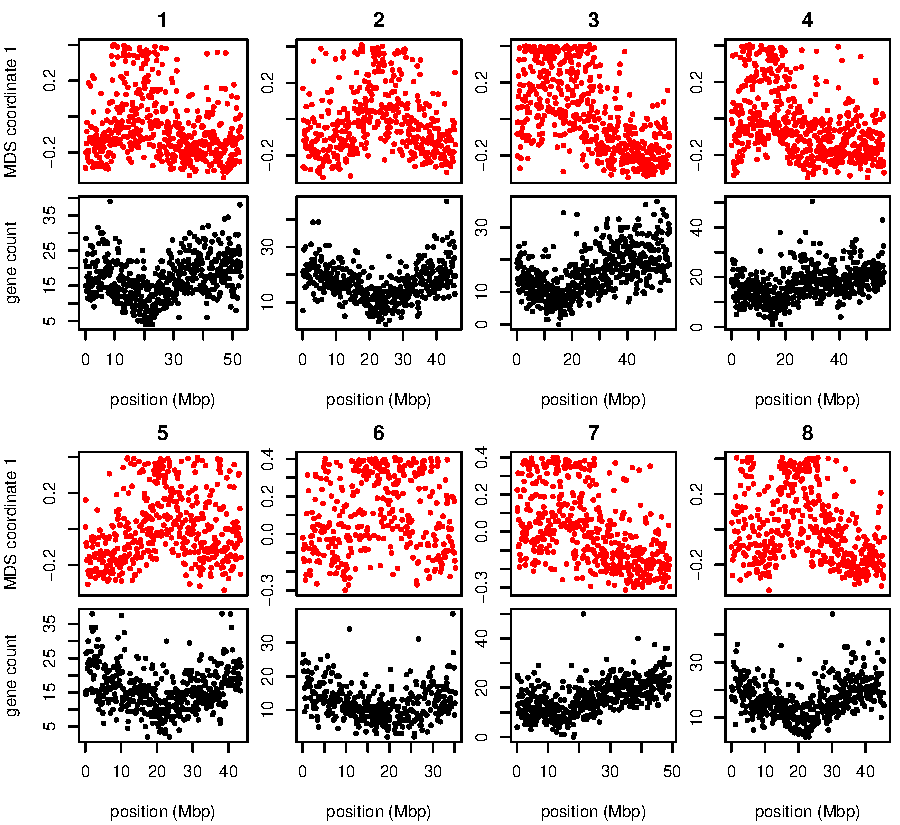
\includegraphics{Fig5_MDS_and_gene_count_allchr_update_correction}
    \end{center}
    \caption{
         MDS coordinate and gene density for each window in the \textit{Medicago} genome,
         for chromosomes 1--8 (numbered above each pair of figures).
         For each chromosome, the red plot above is first coordinate of MDS against the middle position of each window along each chromosome. 
         The black plot below is gene count for each window against the middle position of each window.
         \label{fig:mds_medicago}
    }
\end{figure}

%%%%%%% %%%%%%%%%
\section{Discussion}

Our investigations have found substantial variation in the patterns of relatedness formed by population structure across the genomes
of three diverse species,
revealing distinct biological processes driving this variation in each species.
More investigation, particularly on more species and datasets, will help to uncover what aspects of species history can explain these differences.
With growing appreciation of the heterogeneous effects of selection across the genome,
especially the importance of adaptive introgression and hybrid speciation \citep{pool2015natural,brandvain2014speciation,hufford2013genomic,fitzpatrick2010rapid,staubach2012genome},
local adaptation \citep{lenormand2002limits,wang2014isolation},
and inversion polymorphisms \citep{kirkpatrick2015chromosome,kirkpatrick2010chromosome},
local PCA may prove to be a useful exploratory tool to discover important genomic features.
% It is unclear whether the technique will be useful on reduced representation genotyping datasets 
% due to marker density and issues with missing data --
% our investigations with one such dataset were inconclusive --
% but even low coverage, whole-genome sequence is very promising.

We now discuss possible implications of this variation in the effects of population structure,
the impact of various parameter choices in implementing the method,
and possible additional applications.


\paragraph{Chromosomal inversions}
A major driver of variation in patterns of relatedness in two datasets we examined seems to be inversions.
This may be common,
but the example of \textit{Medicago truncatula} shows that polymorphic inversions are not ubiquitous.
PCA has been proposed as a method for discovering inversions \citep{ma2012investigation};
however, the signal left by inversions likely cannot be distinguished from long haplotypes under balancing selection 
or simply regions of reduced recombination
without additional lines of evidence.  \llabel{ll:inversion_caveat}
Inversions show up in our method because across the inverted region,
most gene trees share a common split that dates back to the origin of the inversion.
However, in many applications, inversions are a nuisance.
For instance, SMARTPCA \citep{patterson2006population} reduces their effect on PCA plots
by regressing out the effect of linked SNPs on each other.
Removing samples with the less common orientation of each inversion reduced,
but did not eliminate, the signal of inversions
seen in the \textit{Drosophila melanogaster} dataset,
demonstrating that the genomic effects of transiently polymorphic inversions
may outlast the inversions themselves.


\paragraph{The effect of selection}
Neutral processes are not expected to produce the chromosome-scale correlations we see in
patterns of relatedness 
in the \textit{Medicago truncatula} and \textit{Drosophila melanogaster} datasets, \llabel{ll:not_neutral}
because correlations induced by neutral processes 
should extend no further than does linkage disequilibrium
(i.e., much less than a chromosome's length).
This suggests that they are produced by linked selection,
a hypothesis backed up by correlations with gene density and recombination rate.
We have also shown with simulations that linked selection can, in at least some circumstances,
produce the sorts of patterns we observe.
How might selection cause variation in patterns of relatedness?
For instance, background selection
(the effect on linked sites of selection against deleterious mutations
\citet{charlesworth1993effect,charlesworth2013background}),
can informally be thought of as reducing the number of potential contributors to the gene pool 
in regions of the genome with many possible deleterious mutations \citep{hudson1995deleterious}.
For this reason, if it acts in a spatial context, it is expected to induce samples from nearby locations to cluster together more frequently.
Therefore, regions of the genome harboring many targets of local adaptation may show similar patterns,
since migrant alleles in these regions will be selected against,
and so locally gene trees will more closely reflect spatial proximity.
Other forms of selection, such as hard sweeps on new mutations,
repeated selection on standing variation, local adaptation,
or temporally fluctuating selection,
could clearly lead to variation 
in geographic patterns of relatedness in a similar way.

Another possible contributor is recent admixture between previously separated populations,
the effects of which were not uniform across the genome due to selection. \revpoint{2}{6}
For instance, it has been hypothesized that large-scale variation in amount of introgressed Neanderthal DNA along the genome
is due to selection against Neanderthal genes, leading to greater introgression in regions of lower gene density
\citep{harris2016genetic,juric2016strength}.
African \textit{Drosophila melanogaster} are thought to have a substantial amount of recently introgressed genome from ``cosmopolitan'' sources;
if selection regularly favors genes from one origin,
this could lead to substantial variation in patterns of relatedness correlated with local gene density.

There has been substantial debate over the relative impacts of different forms of selection
(e.g., \citet{charlesworth1997effects,charlesworth2012effects,pease2013accurate,hedrick2013adaptive,burri2015linked,corbettdetig2015natural,harris2016genetic,martin2016natural,phung2016determining,stankowski2018tempo}). \revpoint{2}{16}
These have been difficult to disentangle in part because for the most part
theory makes predictions which are only strictly valid in randomly mating (i.e., unstructured) populations,
and it is unclear to what extent the spatial structure observed in most real populations will affect these predictions.
It may be possible to design more powerful statistics that make stronger use of spatial information.


% How do we expect selection to affect population structure?
% PCA summarizes patterns in kinship found in the genetic covariance matrix,
% which is an average across locus-specific genealogies:
% if individuals are closer in the genealogies of a given genomic region, 
% they tend to be closer in the PCA maps for that region. 
% Different DNA segments may have different gene tree and therefore different population structure for those segments. 
% Second, the strength of linked selection differs for different DNA segments, and produces different population structure in region under linked selection compared to other region. 
% Selective sweeps cause local recent ancestry or short trees.
% Background selection causes shallow ones.
% Strong selective sweeps of beneficial alleles can lead to relatively long genomic regions
% characterized by short genealogical trees \citep{przeworski2005signature,garud2013selective}.
% A genomic region with many targets for selection experiences
% background selection and/or recurrent selective sweeps \citep{stephan1992effect,coop2012patterns},
% which would tend to shorten genealogical trees in the region,
% similar to a reduction in effective population size \citep{hudson1995deleterious,sattath2011pervasive}.
% % Balancing selection causes deep trees.
% On the other hand, balancing selection leads to very deep trees \citep{gao2014footprints},
% and population structure locally describes which individuals have which alleles
% rather than geographical proximity.
% Finally, 
% since recombination is suppressed between opposite orientations of a chromosomal inversion
% near its breakpoints,
% genealogies in these regions separate samples carrying the two orientations of the inversion.
% In the resulting extended block, population structure shows two (for haploids) or three (for diploids) clusters
% (indeed, \citep{ma2012investigation} has proposed using trimodality of local PCA plots
% as a way to identify inversions).
% if a chromosomal inversion is polymorphic in the sample, 
% the regions around the breakpoints of inversions usually have high linkage disequilibrium and the two directions of a inversion will have different linked alleles around the breakpoints. Recombination suppression across inversions thus results in different genome structure and population structure. 
% Other effects, like noise, introgression might also influence population structure.
% 
% Many of the effects listed above (such as single selective sweeps or inversions) 
% are not expected to have similar effects on population structure in different regions of the genome
% because of randomness in which samples end up in which group;
% but if these coincide with a region of reduced recombination (or an inversion),
% these could drive major patterns of variation.
% The more subtle effects of genome-wide linked selection could be shared across large regions
% due to large-scale variation in gene density
% (as by background selection or local adaptation at many genes).

\paragraph{Parameter choices}
There are several choices in the method that may in principle affect the results.
As with whole-genome PCA,
the choice of samples is important,
as variation not strongly represented in the sample will not be discovered.
The effects of strongly imbalanced sampling schemes are often corrected by dropping samples in overrepresented groups;
but downweighting may be a better option that does not discard data.
Next, the choice of window size may be important,
although in our applications results were not sensitive to this.
Finally, which collections of genomic regions are compared to each other (steps 3 and 4 in \Figure \ref{fig:diagram}),
along with the method used to discover common structure,
will affect results.
We used MDS, applied to either each chromosome separately or to the entire genome;
for instance, human inversions are clearly visible as outliers when compared to the rest of their chromosomes,
but genome-wide, their signal is obscured by the numerous other signals of comparable strength.

Besides window length, there is also the question of how to choose windows.
In these applications we have used nonoverlapping windows with equal numbers of polymorphic sites.
However, we found little change in results when using different window sizes
or when measuring windows in physical distance (in bp).

% More generally, there are many possible methods to discover common structure in different parts of the genome:
% in this work we use PCA to visualize the effects of population structure,
% but other methods, such as STRUCTURE \citep{falush2003inference},
% SPA \citep{yang2012modelbased},
% SpaceMix \citep{bradburd2015spatial},
% or other matrix factorization methods \citep{engelhardt2010analysis}
% may highlight different sources of variation in the data.
% It is also possible that other methods for measuring dissimilarity between windows' covariance matrices
% or for summarizing the matrix of pairwise distances between windows
% would lead to different insights.

Finally, our software allows different choices for how many PCs to use in approximating structure of each window ($k$ in equation \ref{eqn:est_cov}),
and how many MDS coordinates to use when describing the distance matrix between windows,
but in our exploration, changing these has not produced dramatically different results.
These are all part of more general techniques in dimension reduction and high-dimensional data visualization;
we encourage the user to experiment.



\paragraph{Applications}
So-called cryptic relatedness between samples
has been one of the major sources of confounding in genome-wide association studies (GWAS)
and so methods must account for it by modeling population structure or kinship \citep{astle2009population,yang2014advantages}.
Modern ``mixed model'' methods \citep[e.g.][]{loh2015efficient} 
account for this with either a single, genome-wide kinship matrix
or one constructed using only sites unlinked to the focal SNP. \revpoint{2}{9}   %unlike ---> unlink?
Since the effects of population structure is not constant along the genome,
this could in principle lead to an inflation of false positives in parts of the genome
with stronger population structure than the genome-wide average.
A method such as ours might be used to estimate local kinship matrices,
thus providing a more sensitive correction,
although doing so without removing the signal itself could be challenging.
Fortunately, in our human dataset this does not seem likely to have a strong effect:
most variation is due to small, independent regions, possibly primarily inversions,
and so may not have a major effect on GWAS.
In the other species we examined, particularly \textit{Drosophila melanogaster},
treating population structure as a single quantity would entail a substantial loss of power,
and could potentially be misleading.

%%%%%%%%
\section*{Acknowledgements}

We are indebted to John Pool, Russ Corbett-Detig, Matilde Cordeiro, and Peter Chang 
for assistance with obtaining data and interpreting results
(especially inversion status of \textit{D.~melanogaster} samples).
Jaime Ashander and Jerome Kelleher provided assistance in performing the simulations.
Thanks also go to Yaniv Brandvain, Barbara Engelhardt, Charles Langley, Graham Coop, and Jeremy Berg for helpful comments
and for encouraging the project.

%%%%%%%%
\section*{Disclosure declaration}

The authors declare no conflicts of interest.


\bibliography{references}  
\ifsubmission
    \clearpage
    \newcounter{bibend}
    \setcounter{bibend}{\value{page}}
\fi

\ifsubmission\processdelayedfloats\fi

\ifsubmission
    \clearpage
    \setcounter{page}{\thebibend}
\fi

\appendix
\setcounter{table}{0}
\renewcommand{\thetable}{S\arabic{table}}
\setcounter{figure}{0}
\renewcommand{\thefigure}{S\arabic{figure}}
\ifsubmission
    \setcounter{postfigure}{0}
    \renewcommand{\thepostfigure}{S\arabic{postfigure}}
\fi

\section{Choosing window length}
\label{apx:window_length}

The choice of window length entails a balance between signal and noise.
In very short windows, genealogies of the samples will only be represented by a few trees,
so variation between windows represents demographic noise rather than meaningful variation in patterns of relatedness.
Longer windows generally have more distinct trees (and SNPs), 
allowing for less noisy estimation of local patterns of relatedness.
However, to better resolve meaningful signal, i.e., differences in patterns of relatedness along the genome,
we would like reasonably short windows.
% Window length choice therefore entails a signal versus noise tradeoff
% in the estimates of population structure.
% If we use the first principal component as a measure of population structure, 
% then to choose the best window length,
% we need to find a balance between the standard error of the first principal components for each window 
% and the standard deviation between windows. 

Since we summarize patterns of relatedness using relative positions in the principal component maps,
we quantify ``noise'' as the standard error of a sample's position on PC1 in a particular window,
averaged across windows and samples,
and ``signal'' as the standard deviation of the sample's position on PC1 over all windows,
averaged over samples. \revpoint{2}{11}
The definition of eigenvectors does not specify their sign,
and so when comparing between windows we choose signs to best match each other:
after choosing $\pcone_1$, for instance, 
if $u$ is the first eigenvector obtained from the covariance matrix
for window $j$,
then we next choose $\pcone_j = \pm u$,
where the sign is chosen according to which of 
$\| \pcone_{1} - u \|$ or
$\| \pcone_{1} + u \|$ 
is smaller.
\llabel{ll:moved_pc_note}

After doing this, the mean variance across windows is
\begin{align*}
    \sigma_\text{signal}^2
    = 
    \frac{1}{N} \sum_{j=1}^{N}
        \frac{1}{L}\sum_{i=1}^{L}\left ( \pcone_{ij} -\overline\pcone_{j} \right )^{2} ,
\end{align*}
where $\pcone_{ij}$ is the position of the $i^\text{th}$ individual on $\pcone$ in window $j$,
and $\overline\pcone_j = (1/N) \sum_{j=1}^N \pcone_{ij}$.
We estimate the standard error for each $\pcone_{ij}$ using the block jackknife \citep{efron1982jackknife,busing1999deletem}: \revpoint{2}{5}
we divide the $j^\text{th}$ window into 10 equal-sized pieces,
and let $\pcone_{ij,k}$ denote the first principal component of this region found after removing the $k^\text{th}$ piece;
then the estimate of the squared standard error is
$\sigma^2_{ij} = \frac{9}{10} \sum_{k=1}^{10} ( \pcone_{ij,k} - \frac{1}{10} \sum_{\ell=1}^{10} \pcone_{ij,\ell} )^2$.
Averaging over samples and windows,
\begin{align*}
    \sigma^2_\text{noise}
    &=
    \frac{1}{N} \sum_{j=1}^{N} \frac{1}{L}\sum_{i=1}^{L} \sigma^2_{ij} .
\end{align*}

For the main analysis, we defined windows to each consist of the same number of neighboring SNPs,
and calculated $\sigma^2_\text{signal}$ and $\sigma^2_\text{noise}$
for a range of window sizes (i.e., numbers of SNPs).
For our main results we
chose the smallest window for which $\sigma^2_\text{signal}$ was consistently larger than $\sigma^2_\text{noise}$ (but checked other sizes);
the values for various window sizes across \textit{Drosophila} chromosomes are shown in Table \ref{tab:window_sizes}.
% and the choices for all taxa are in Table \ref{tab:data_stats}.
% In practice, even substantially different window sizes result in the same genome-wide patterns.
In the cases we examined, we found nearly identical results after varying window size,
and choosing windows to be of the same physical length (in bp) rather than in numbers of SNPs.

% # Variances within and between windows for Drosophila, multiplied by 1000:
% w <- structure(list(chrom = structure(c(1L, 1L, 2L, 2L, 3L, 3L, 4L, 
% 4L, 5L, 5L), .Label = c("2L", "2R", "3L", "3R", "X"), class = "factor"), 
%     type = structure(c(1L, 2L, 1L, 2L, 1L, 2L, 1L, 2L, 1L, 2L
%     ), .Label = c("noise", "signal"), class = "factor"), `100` = c(2.05209, 
%     2.75625, 2.18089, 2.77729, 2.07936, 2.601, 1.95364, 2.58064, 
%     2.48004, 2.61121), `500` = c(1.64025, 2.69361, 1.91844, 2.704, 
%     1.99809, 2.52004, 1.764, 2.51001, 2.04304, 2.43049), `1000` = c(1.18336, 
%     2.22784, 1.63216, 2.65225, 1.64025, 2.401, 1.43641, 2.44036, 
%     1.53664, 2.304), `10000` = c(0.169, 0.676, 0.576, 2.31361, 
%     0.73441, 1.681, 0.58564, 1.96249, 1.61604, 0.324), `1e+05` = c(0.03969, 
%     0.31329, 0.13456, 1.82329, 0.24649, 1.89225, 0.20164, 1.39876, 
%     0.169, 1.14244)), .Names = c("chrom", "type", "100", "500", 
% "1000", "10000", "1e+05"), row.names = c(NA, -10L), class = "data.frame")
% print(xtable(w),include.rownames=FALSE)

\begin{table}[ht]
\centering
    \begin{tabular}{cccrrrrr}
  \hline
        & & & \multicolumn{5}{c}{window length (SNPs)} \\
 & chrom.\ arm  & & 100 & 500 & 1,000 & 10,000 & 100,000 \\ 
  \hline
    & 2L & $\sigma^2_\text{noise}$  & 2.05  &  1.64  &  1.18  &  0.17  &  0.04 \\
    & 	 & $\sigma^2_\text{signal}$ & 2.76  &  2.69  &  2.23  &  0.68  &  0.31 \\
    & 2R & $\sigma^2_\text{noise}$  & 2.18  &  1.92  &  1.63  &  0.58  &  0.13 \\
    & 	 & $\sigma^2_\text{signal}$ & 2.78  &  2.70  &  2.65  &  2.31  &  1.82 \\
    & 3L & $\sigma^2_\text{noise}$  & 2.08  &  2.00  &  1.64  &  0.73  &  0.25 \\
    & 	 & $\sigma^2_\text{signal}$ & 2.60  &  2.52  &  2.40  &  1.68  &  1.89 \\
    & 3R & $\sigma^2_\text{noise}$  & 1.95  &  1.76  &  1.44  &  0.59  &  0.20 \\
    & 	 & $\sigma^2_\text{signal}$ & 2.58  &  2.51  &  2.44  &  1.96  &  1.40 \\
    & X  & $\sigma^2_\text{noise}$  & 2.48  &  2.04  &  1.54  &  1.62  &  0.17 \\
    & 	 & $\sigma^2_\text{signal}$ & 2.61  &  2.43  &  2.30  &  0.32  &  1.14 \\
   \hline
\end{tabular}
\caption{
    Measures of signal and noise,
    computed separately for each chromosome arm in the \textit{Drosophila} dataset,
    at different window sizes.
    All values are multiplied by $1,000$.
    Starting at windows of 1,000 SNPs, the signal (variation of PC1 between windows)
    starts to be substantially larger than the noise (standard error of PC1 for each window).
} \label{tab:window_sizes}
\end{table}


%%%%%%%%%%%%%%%%%%%%%
\section{Simulations}

We implemented two types of simulation:
first, simple simulations of Gaussian ``genotypes'' 
where the expectation of variation in ``population structure'' was clear;
and next, individual-based simulations with explicit genomes, using SLiM.

%%%%%%%%%%%%%%%%%%%%%%%%%%%%%%%%%
\subsection{Gaussian simulations}
\label{apx:gaussian_sims}

We simulated genotypes at each locus independently,
drawing each vector of genotypes from a multivariate Gaussian distribution
with zero mean and covariance matrix $\Sigma$.
Sampled individuals came from three populations,
and each $\Sigma_{ij}$ depends on which populations the individuals $i$ and $j$ are in,
as well as the location along the chromosome.
There are three population-level mean relatedness matrices along the genome,
which apply to the first quarter ($S^{(1)}$),
the middle half ($S^{(2)}$),
and the last quarter ($S^{(3)}$), respectively:
\begin{align*}
    S^{(1)} &= 
    \begin{bmatrix}
        0.75 &  0.25 &  0.0 \\
        0.25 &  0.75 &  0.0 \\
        0.0  &  0.0  &  1.0 \\
    \end{bmatrix} \\
    S^{(2)} &= 
    \begin{bmatrix}
        1.0  &  0.0  &  0.0 \\
        0.0  &  0.75 &  0.25\\
        0.0  &  0.25 &  0.75\\
    \end{bmatrix} \\
    S^{(3)} &= 
    \begin{bmatrix}
        0.75 &  0.0  &  0.25\\
        0.0  &  1.0  &  0.0 \\
        0.25 &  0.0  &  0.75\\
    \end{bmatrix} \\
\end{align*}
If indiviudals $i$ and $j$ are in populations $p(i)$ and $p(j)$ respectively,
then the covariance between their genotypes is $\Sigma_{ij} = S_{p(i),p(j)}$, 
using the appropriate $S$ for that segment of the genome.
The variance of individual $i$'s genotype is $\Sigma_{ii} = S_{p(i),p(i)} + 0.1$.

We first created ``genotypes'' in this way with fifty individuals from each of the three populations;
running our method on a genome with 99 windows of 400 loci each
produced the first plot in Figure \ref{sfig:test_missing}.
These matrices are chosen so that the top two eigenvalues $\Sigma$ are the same (both 50.1),
and so the ordering of the top two PCs is arbitrary.
If our method was sensitive to PC ordering,
then half the windows in each region that have one ordering would cluster with each other,
separate from the other half. \llabel{ll:pc_switching_test}

We then marked each genotype in the first half of the chromosome
as missing, independently, with probability $1/2$ and ran our method again,
producing the second plot of Figure \ref{sfig:test_missing}. \llabel{ll:test_missing}
If our method was influenced by missing data,
we would expect the first half of the chromosome to separate from the second
in the MDS plot.

%%%%%%%%%%%%%%%%%%%%%%%%%%%%%%%%%
\subsection{SLiM simulations}
\label{apx:slim_sims}

Our SLiM simulations were constructed as follows.
Individuals are diploid, and genomes have a length of 153,520,244 bp.
Recombination was either 
(a) flat, with a constant rate of $10^{-9}$;
(b) according to the human female HapMap map for chromosome 7;
or (c) constant in each of seven equal-sized regions, beginning at $2.04\times 10^{-8}$,
descending by a factor of four for three steps, and then ascending by a factor of four for three steps,
so that the middle seventh has the lowest recombination rate,
and the outer two sevenths has a rate 64 times higher.
Selected mutations are introduced at a rate of $10^{-10}$ per bp per individual per generation,
and have selection coefficients drawn from a Gamma distribution with mean 0.005 and shape 2;
each coefficient are either positive or negative with probabilities $1/30$ and $29/30$ respectively.
Each simulation was run for 50,000 generations.

Each individual has a spatial position in the two-dimensional square of width $W=8$.
Each time step, each individual chooses the nearest other to mate with,             
producing a random, Poisson distributed number of offspring with mean $1/3$.
Offspring are assigned random spatial locations displaced from their parent's
by a bivariate Gaussian with mean zero and standard deviation $\sigma = 0.2$,
reflected to stay within the habitat range.

Each individual survives to the next time step
with probability equal to their fitness.
Fitness values are determined multiplicatively by the effects of each mutation,
but are multiplied by an additional factor determined by the local density of individuals.
This factor is equal to $\rho / (1 + C)$,
where $\rho = 2 \pi K \sigma^2$ is the carrying capacity per circle of radius $\sigma$;
$K=100$ is the mean equilibrium population density;
and $C$ is the sum of a Gaussian kernel with standard deviation $\sigma = 0.1$
between the focal individual and all other individuals within distance $3 \sigma$.
To avoid edge effects, fitnesses are further multiplied by $\min(1, z)$,
where $z$ is the distance to the nearest boundary.
This produces populations that fluctuate at equilibrium around 6,000 individuals in total,
fairly evenly spread across the square.

In one additional simulation, we modified fitnesses by multiplying the selective effect
of each allele in each individual by multiplying it by $2x/W - 1$, 
where $x$ is the $x$ coordinate of the individual.
This makes the effect of each allele opposite on the left and on the right,
and neutral in the middle,
and leads to a moderate number of balanced polymorphisms.


% put in list of figures here 
\ifsubmission
    \listoffigures
    \clearpage
\fi

\section{Supplementary Tables}

% latex table generated in R 3.3.1 by xtable 1.8-2 package
% Wed Feb  8 16:17:12 2017
\begin{table}[ht]
\centering
    \begin{tabular}{rrrrrr}
      \hline
          & 10000 SNPs & 1000 SNPs & 10000 SNPs & 100000bp & 10000bp \\ 
     MDS1 & 2 PCs & 2 PCs & 5 PCs & 2 PCs & 2 PCs \\ 
      \hline
  10000 SNPs, 2 PCs & 1.00 & 0.87 & 0.96 & 0.90 & 0.88 \\ 
  1000 SNPs, 2 PCs & 0.68 & 1.00 & 0.73 & 0.68 & 0.94 \\ 
  10000 SNPs, 5 PCs & 0.96 & 0.92 & 1.00 & 0.88 & 0.93 \\ 
  100000bp, 2 PCs & 0.90 & 0.87 & 0.88 & 1.00 & 0.87 \\ 
  10000bp, 2 PCs & 0.68 & 0.93 & 0.72 & 0.67 & 1.00 \\ 
       \hline
       \hline
        MDS2 & &&&&\\
      \hline
      10000 SNPs, 2 PCs & 1.00 & 0.54 & 0.93 & 0.87 & 0.56 \\ 
      1000 SNPs, 2 PCs & 0.82 & 1.00 & 0.76 & 0.83 & 0.92 \\ 
      10000 SNPs, 5 PCs & 0.93 & 0.50 & 1.00 & 0.83 & 0.52 \\ 
      100000bp, 2 PCs & 0.87 & 0.59 & 0.84 & 1.00 & 0.58 \\ 
      10000bp, 2 PCs & 0.83 & 0.92 & 0.77 & 0.84 & 1.00 \\ 
       \hline
    \end{tabular}
    \caption{
        Correlations between MDS coordinates of genomic regions
        between runs with different parameter values.
        To produce these, 
        we first ran the algorithm with the specified window size and number of PCs 
        ($k$ in equation \eqref{eqn:est_cov})
        on the full \textit{Medicago truncatula} dataset.
        Then to obtain the correlation between results obtained from parameters A in the row of the matrix above
        and parameters B in the column of the matrix above,
        we mapped the windows of B to those of A by averaging MDS coordinates of any windows of B whose midpoints lay in the corresponding window of A;
        we then computed the correlation between the MDS coordinates of A and the averaged MDS coordinates of B.
        This is not a symmetric operation, so these matrices are not symmetric.
        As expected, parameter values with smaller windows produce noisier estimates,
        but plots of MDS values along the genome are visually very similar.
    } \label{tab:param_cors}
\end{table}

\section{Supplementary Figures}


\begin{figure}
    \begin{center}
       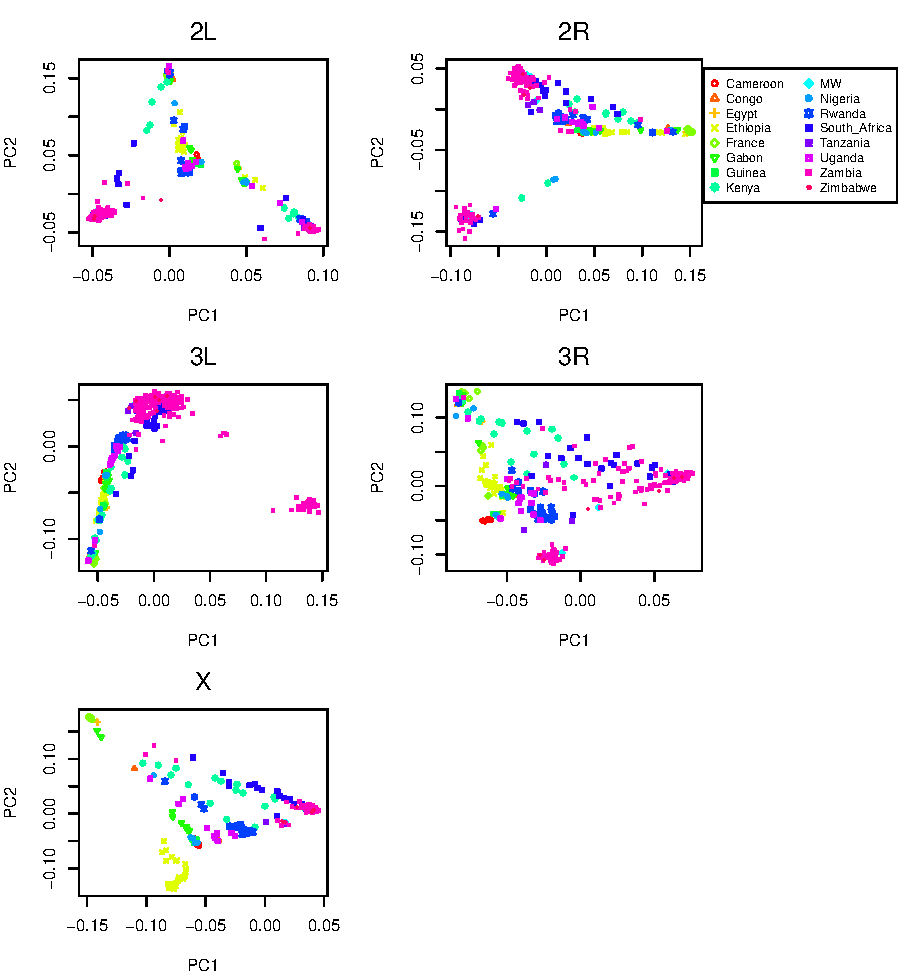
\includegraphics[width=1\textwidth]{FigS_pca_plots_allchr_drosophila}
    \end{center}
    \caption{
        PCA plots for chromosome arms 2L, 2R, 3L, 3R and X of the \textit{Drosophila melanogaster} dataset.
        \label{sfig:pca_drosophila_allchr}
    }
\end{figure}

\begin{figure}
    \begin{center}
        \ifusepngs
           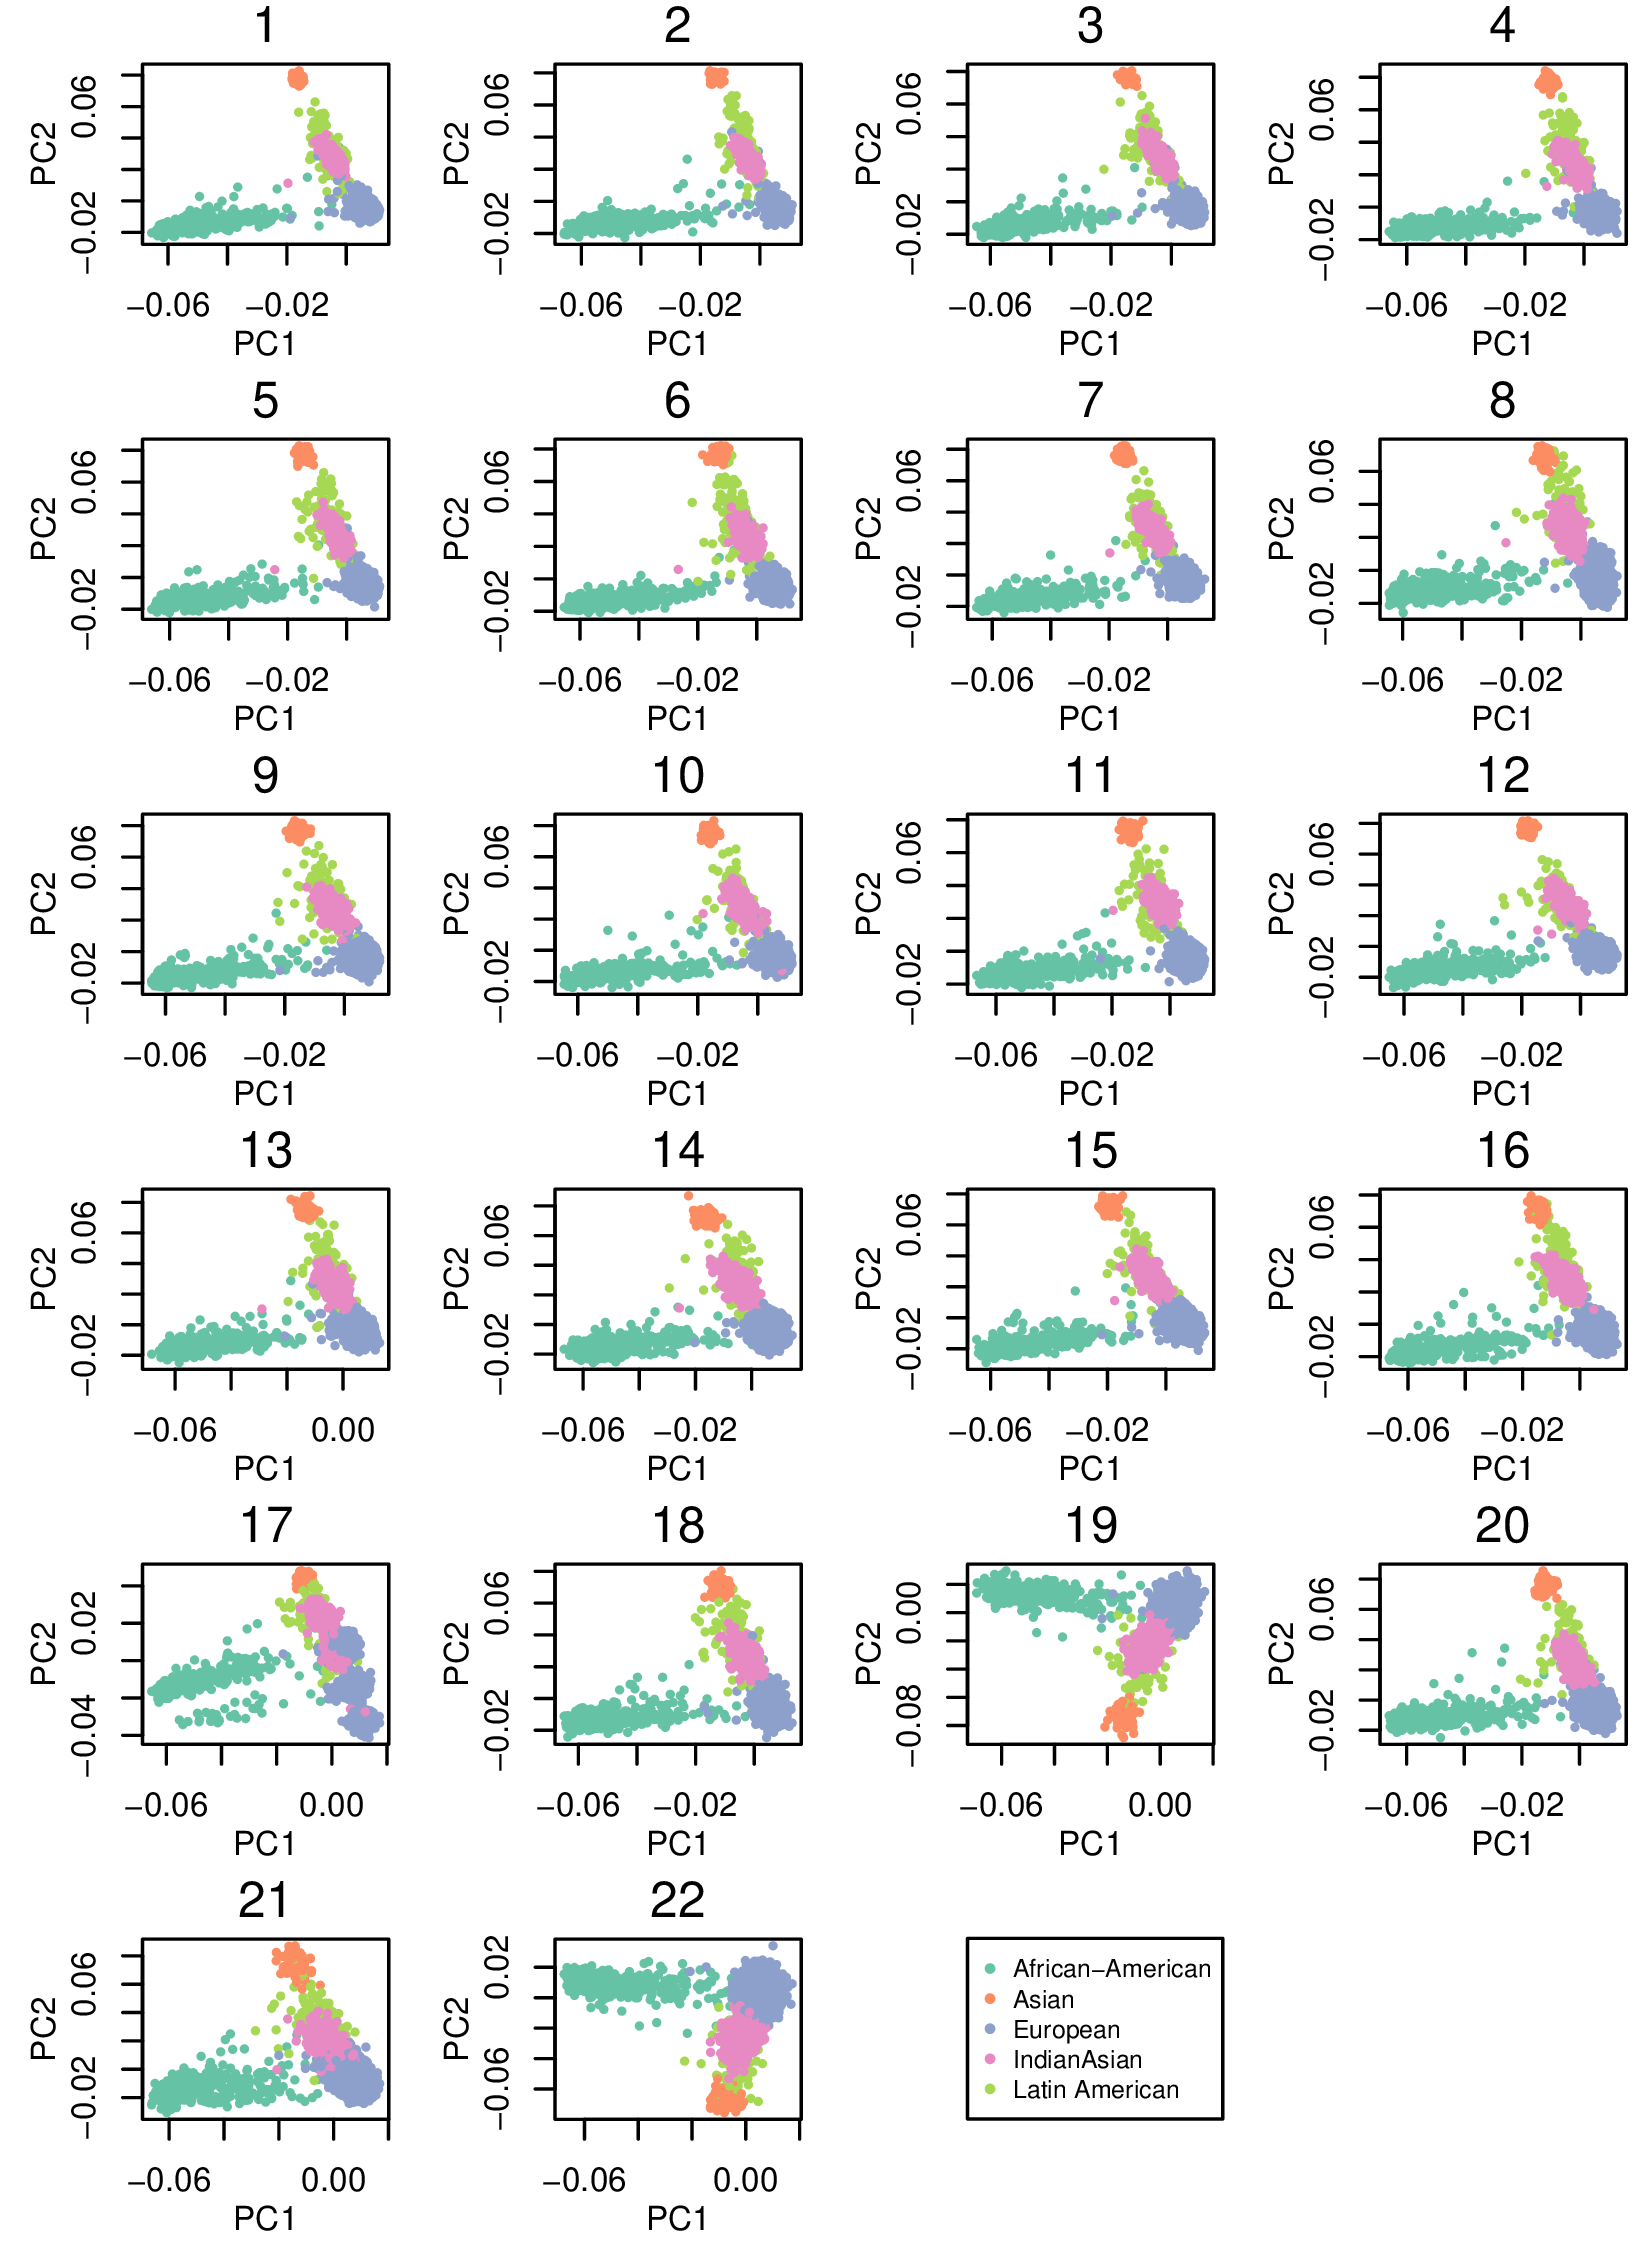
\includegraphics[width=0.9\textwidth]{FigS_pca_plot_allchr_human.png}
       \else
           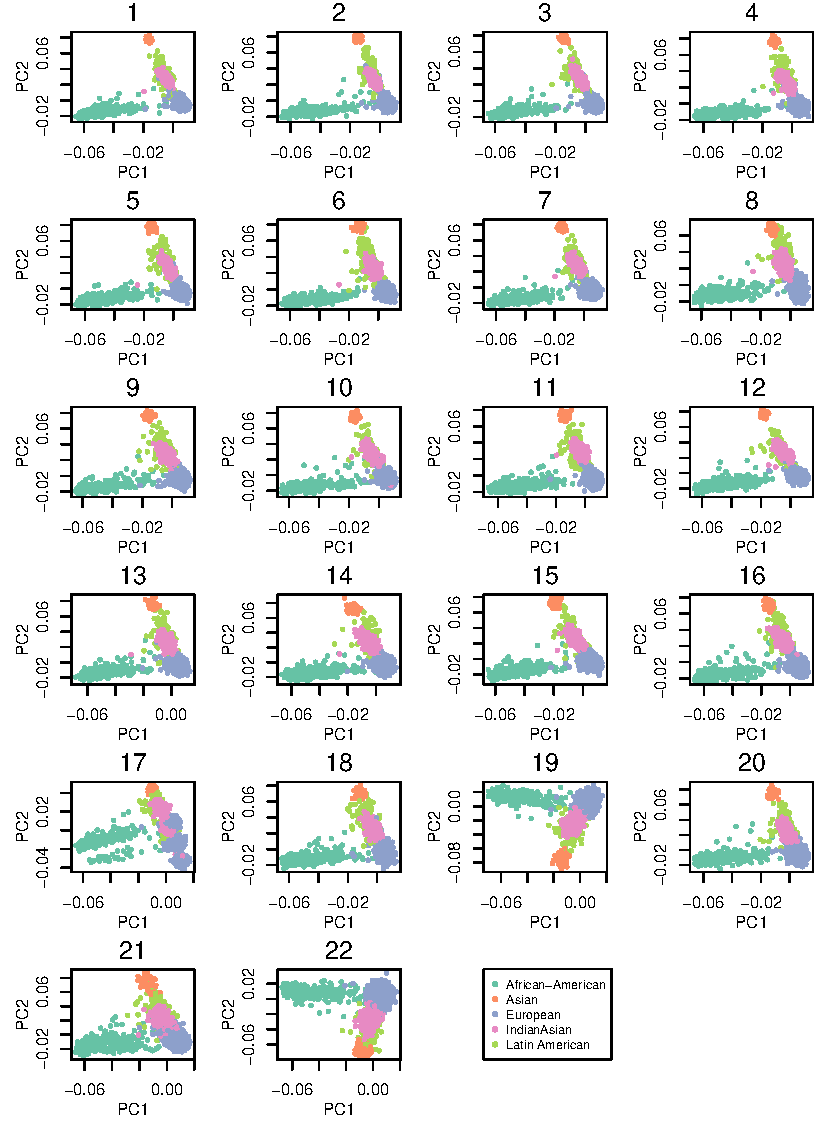
\includegraphics[width=0.9\textwidth]{FigS_pca_plot_allchr_human}
       \fi
    \end{center}
    \caption{
        PCA plots for all 22 human autosomes from the POPRES data.
        \label{sfig:pca_human_allchr}
    }
\end{figure}

\begin{figure}
    \begin{center}
       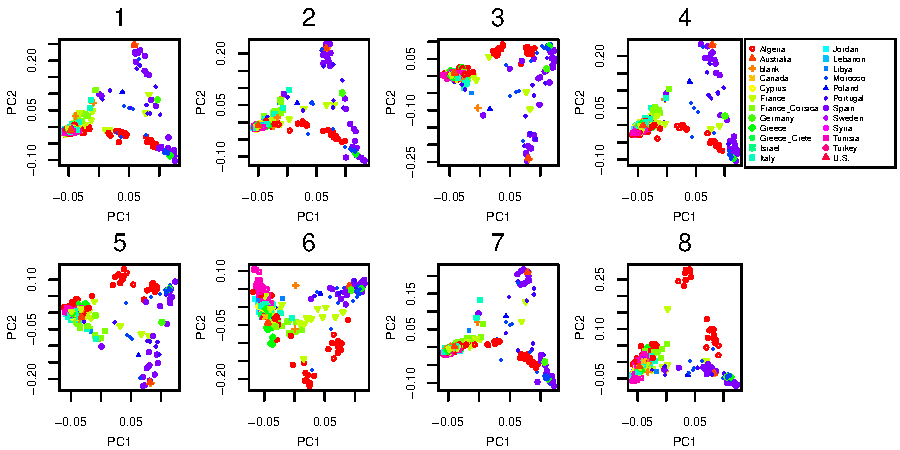
\includegraphics[width=1\textwidth]{FigS_pca_plots_medicago_allchr}
    \end{center}
    \caption{
        PCA plots for all 8 chromosomes in the \textit{Medicago truncatula} dataset.
        \label{sfig:pca_medicago_allchr}
    }
\end{figure}

%%%%%%%%%%simulations

\begin{figure}
    \begin{center}
        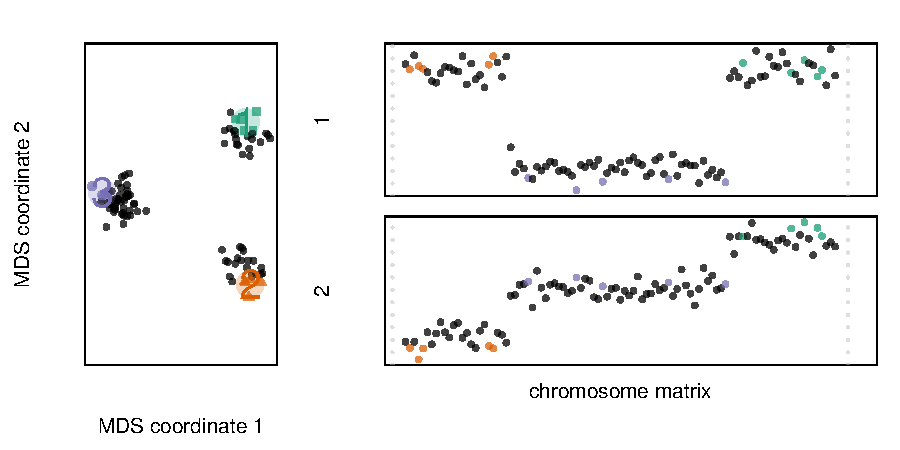
\includegraphics[width=0.82\textwidth]{simple_example_base_case}
        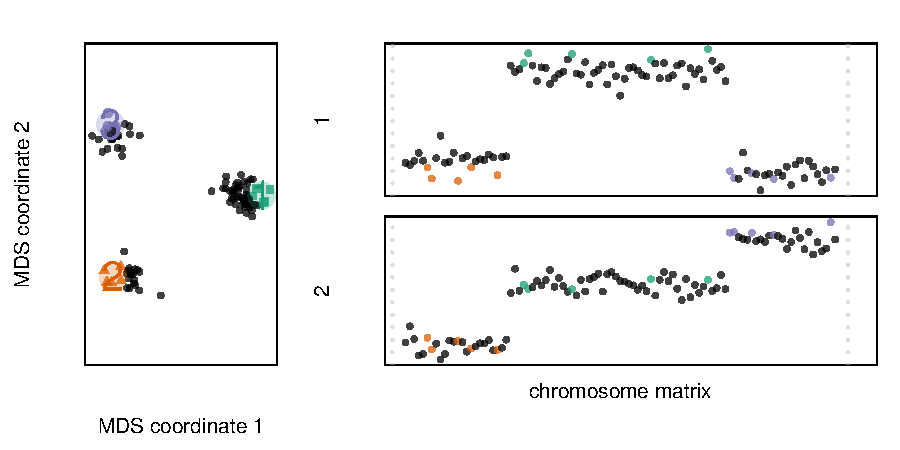
\includegraphics[width=0.82\textwidth]{simple_example_missing_data}
    \end{center}
    \caption{
        MDS visualizations of the Gaussian genotypes described in Appendix \ref{apx:gaussian_sims},
        for 50 individuals from each of three populations.
        \textbf{(top)} The first quarter, middle half, and final quarter of the chromosome
        each have different population structure, as expected,
        despite the possibility for PC switching within each.
        \textbf{(bottom)} The same picture results even after marking a random 50\% of the genotypes
        in the first half of the chromosome as missing.
    } \label{sfig:test_missing}.
\end{figure}

\begin{figure}
    \begin{center}
       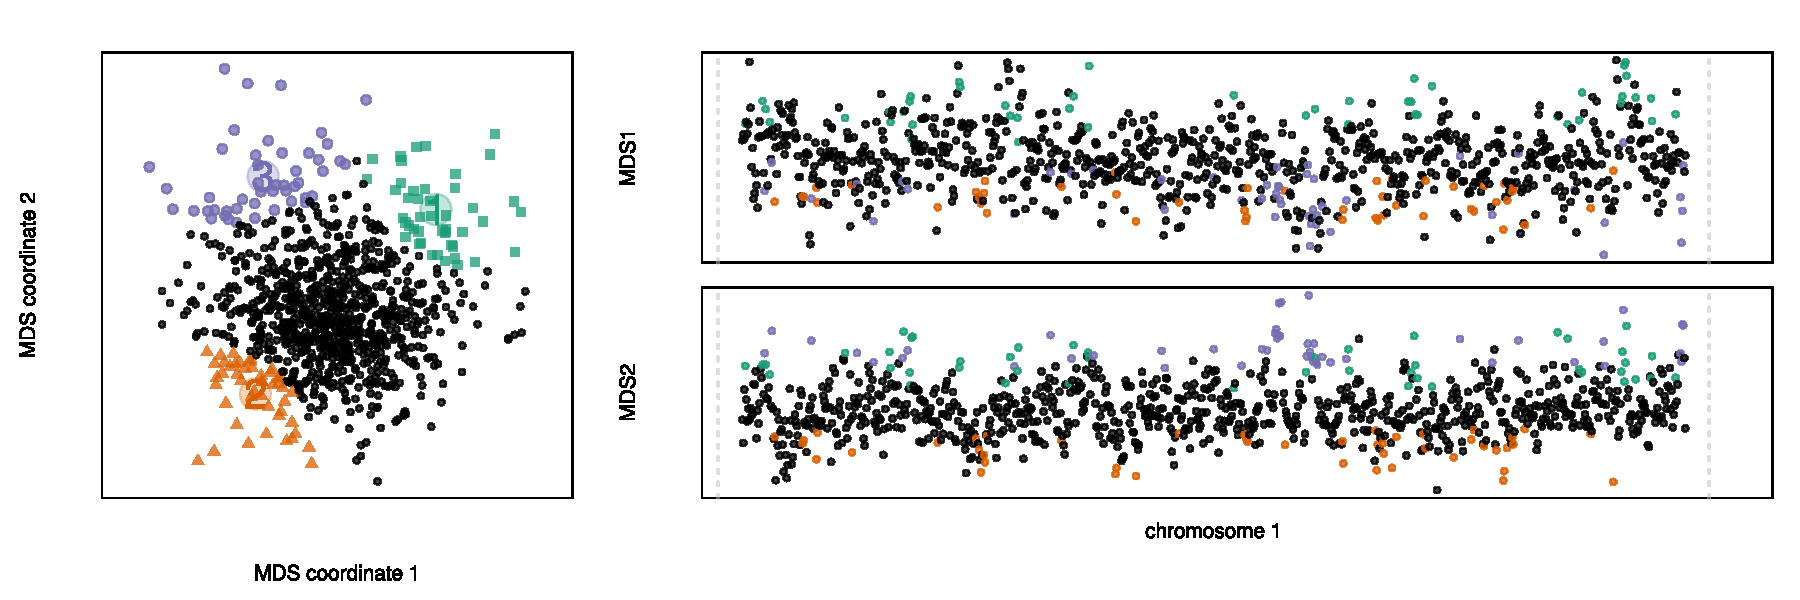
\includegraphics[width=0.82\textwidth]{FigS_plot_corners-1_run_027034}
       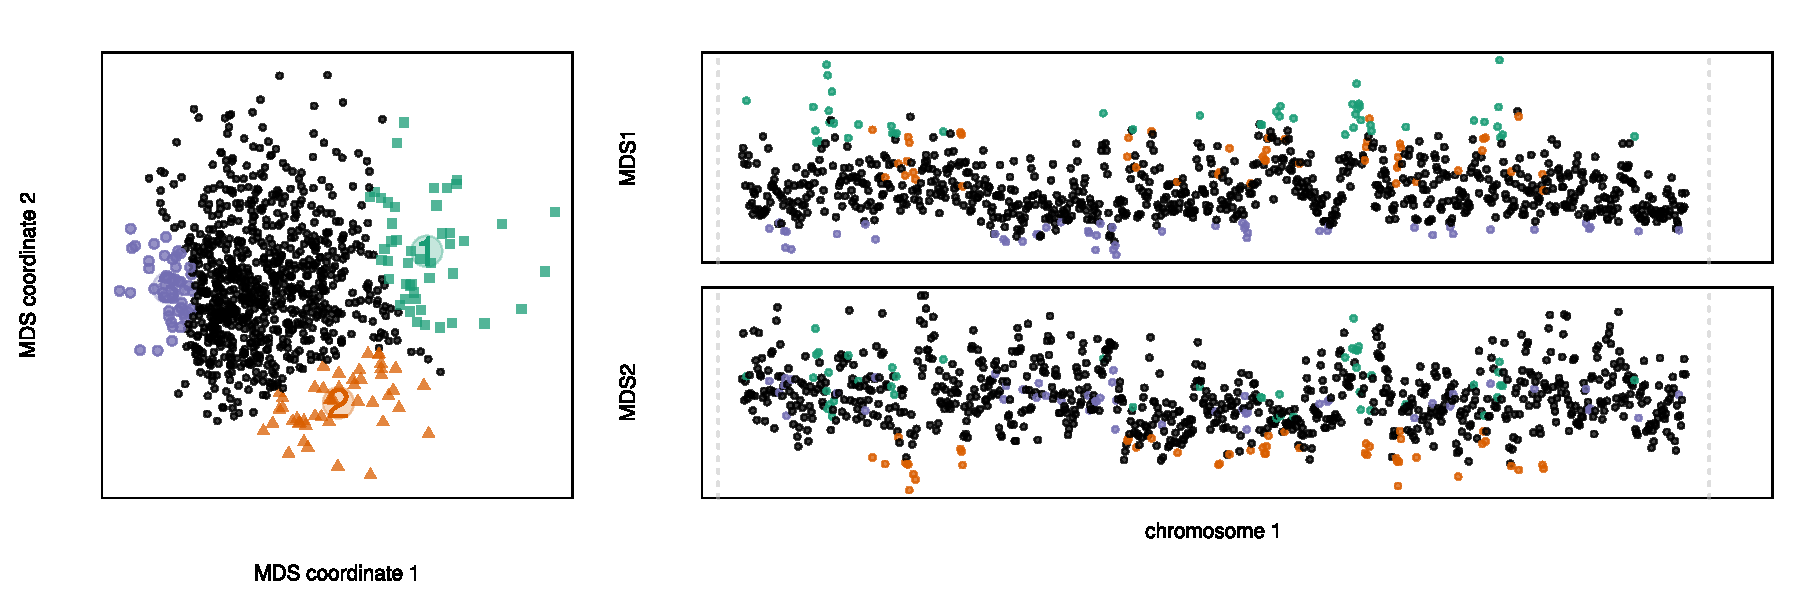
\includegraphics[width=0.82\textwidth]{FigS_plot_corners-1_run_012720}
       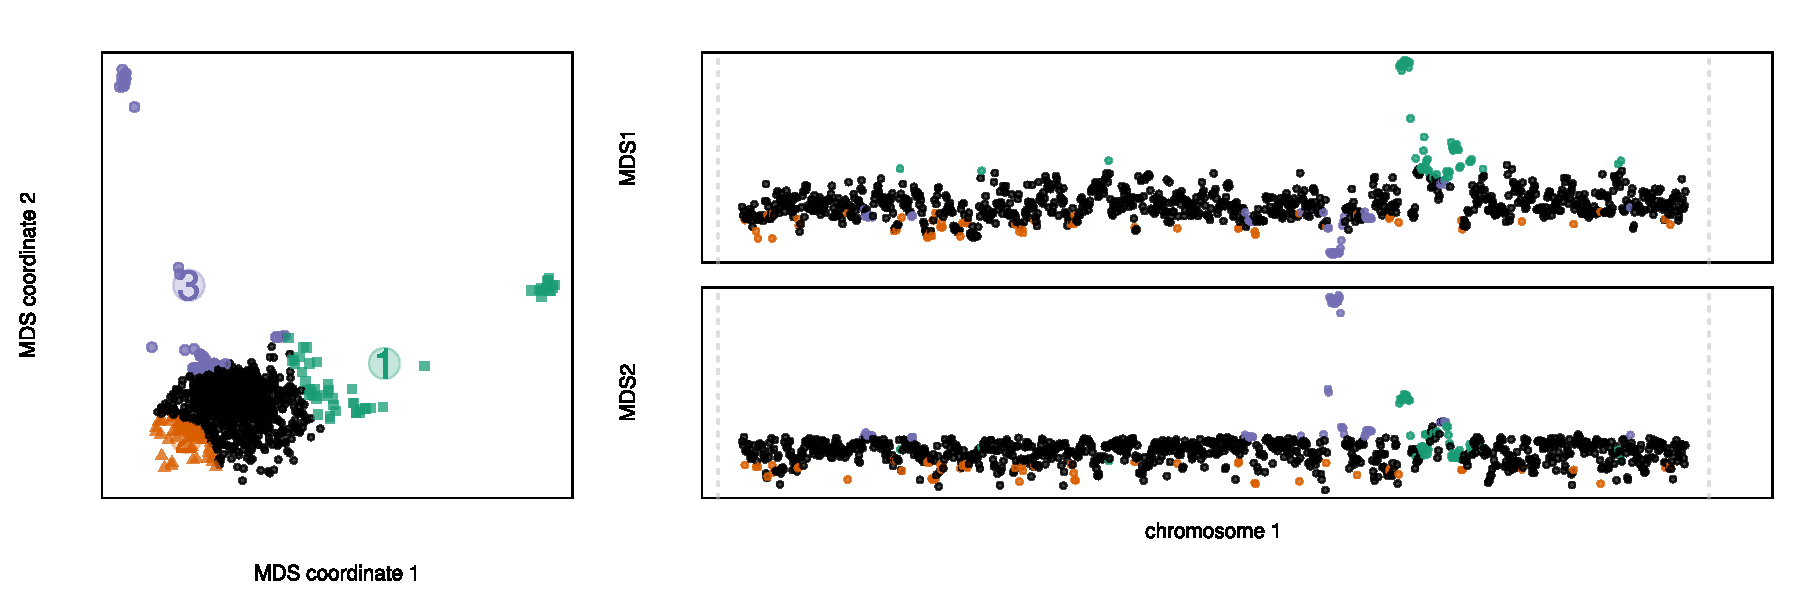
\includegraphics[width=0.82\textwidth]{FigS_plot_corners-1_run_015598}
       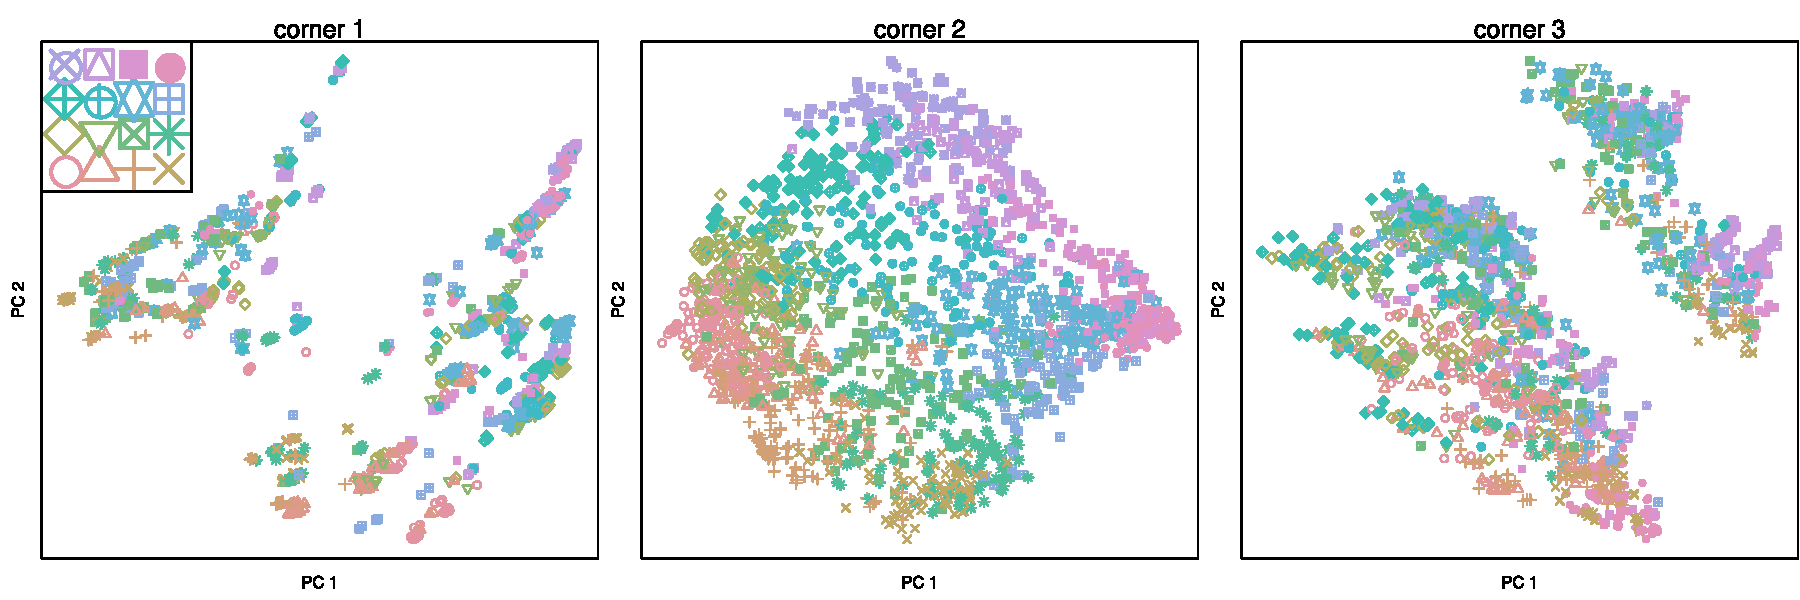
\includegraphics[width=0.82\textwidth]{FigS_plot_corner_pca-1_run_015598}
    \end{center}
    \caption{
        MDS visualizations of the results of individual-based simulations using SLiM
        (see Appendix \ref{apx:slim_sims} for details).
        All simulations are neutral, and recombination is:
        \textbf{(top)} constant;
        \textbf{(top middle)} varies stepwise by factors of two in seven equal-length segments,
        with highest rates on the ends, so the middle segment has a recombination rate 64 times lower
        than the ends;
        \textbf{(bottom middle)} according to the HapMap human female chromosome 7 map.
        The \textbf{bottom} figure shows PCA maps corresponding to the three colored windows
        of the last (HapMap) situation;
        the outlying regions are long regions of low recombination rate,
        so that region can be dominated by a few correlated trees,
        similar to an inversion.
    } \label{sfig:slim_sims1}
\end{figure}


\begin{figure}
    \begin{center}
       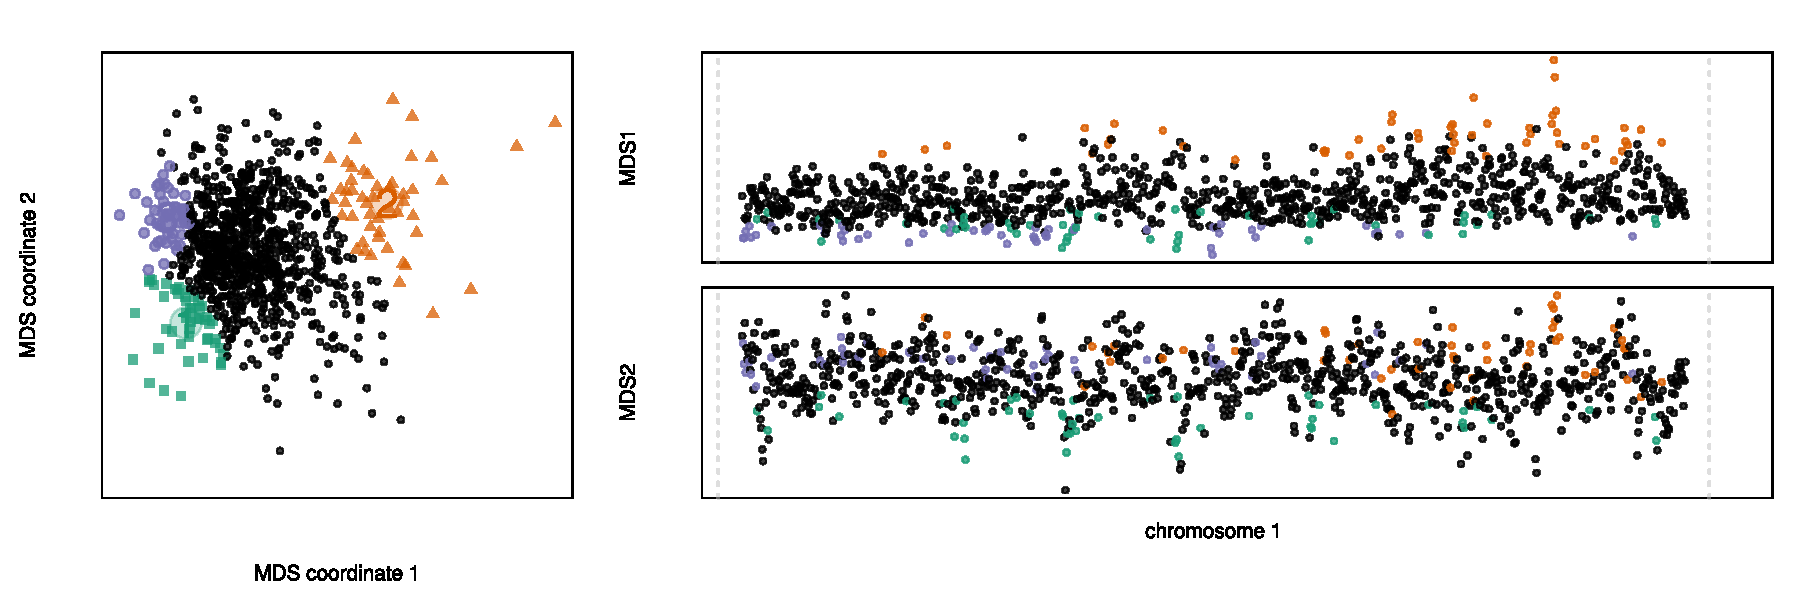
\includegraphics[width=0.82\textwidth]{FigS_plot_corners-1_run_031486} % base, selected
       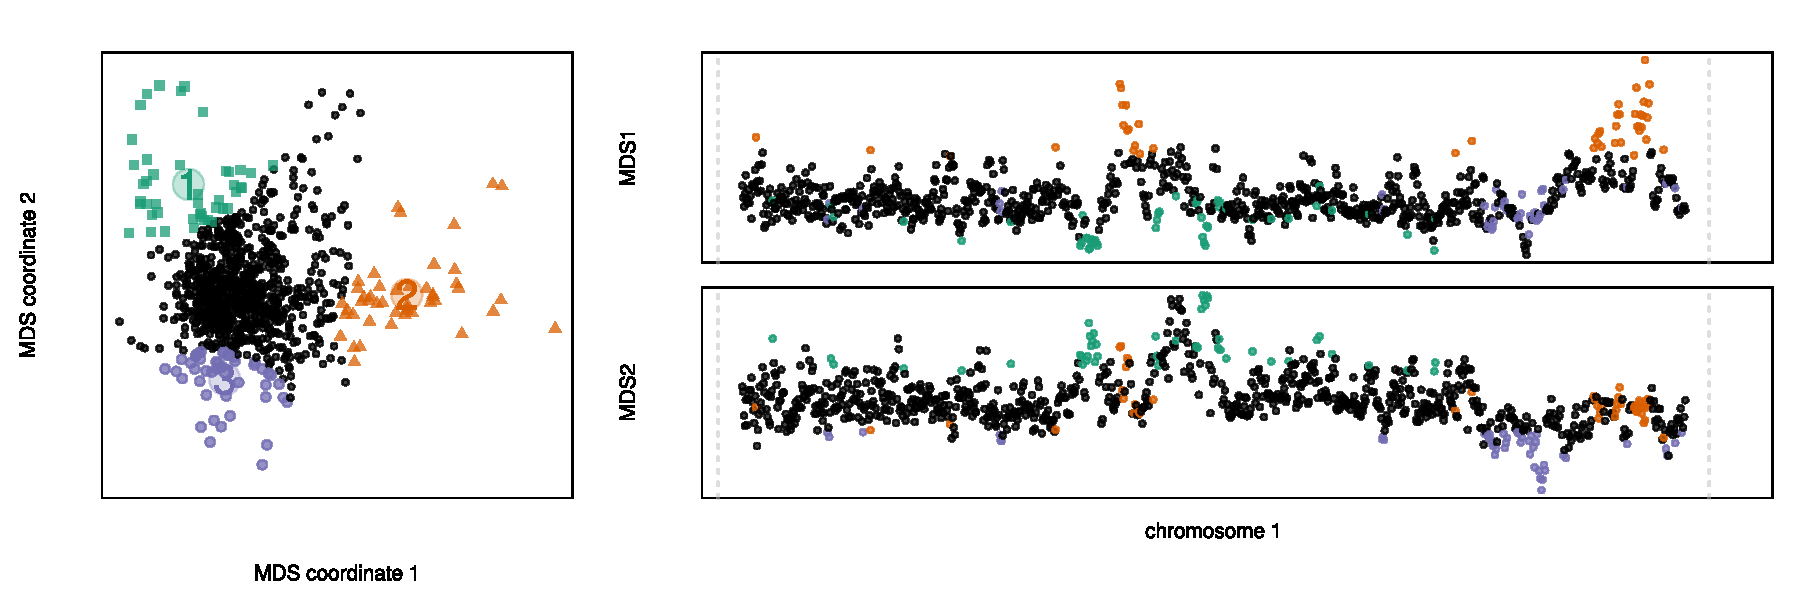
\includegraphics[width=0.82\textwidth]{FigS_plot_corners-1_run_009673} % step, selected
       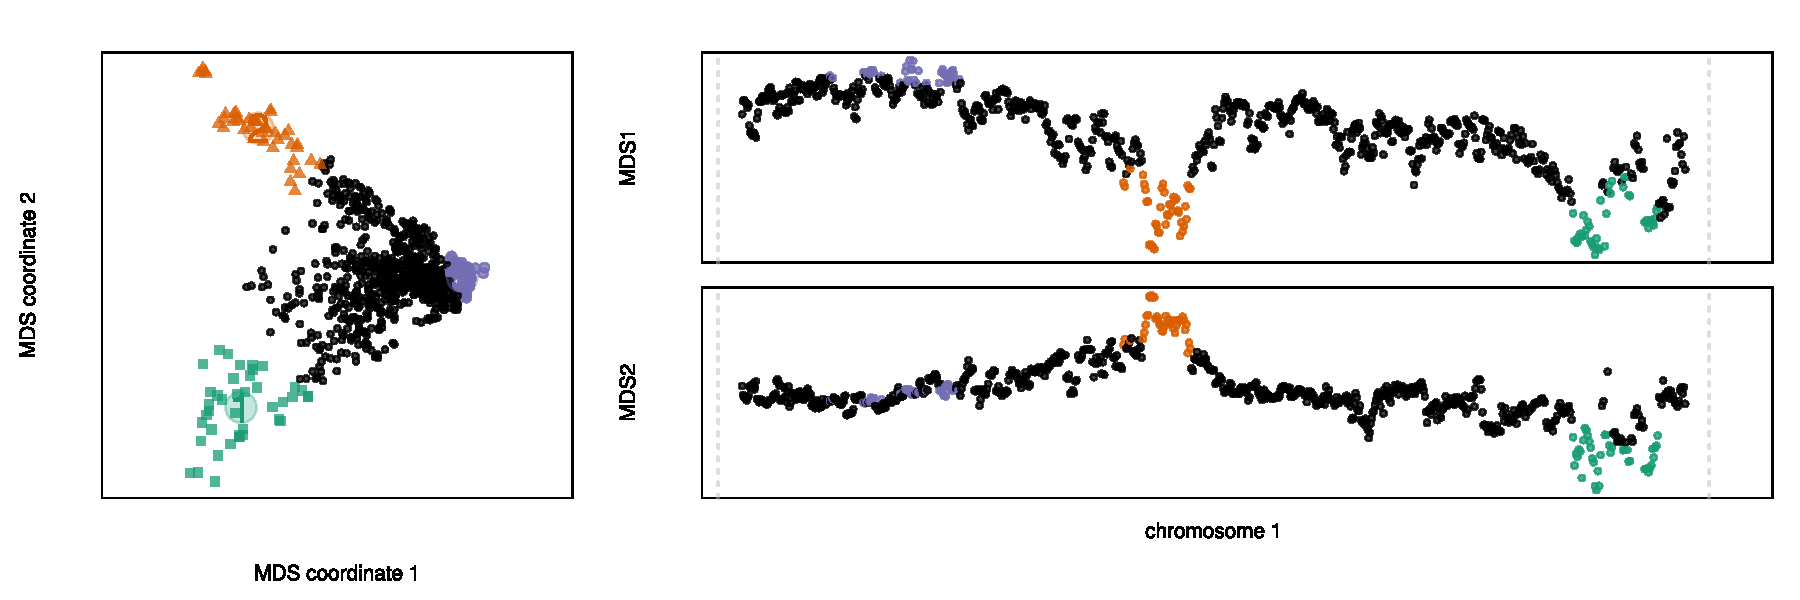
\includegraphics[width=0.82\textwidth]{FigS_plot_corners-1_run_016913} % base, balancing
       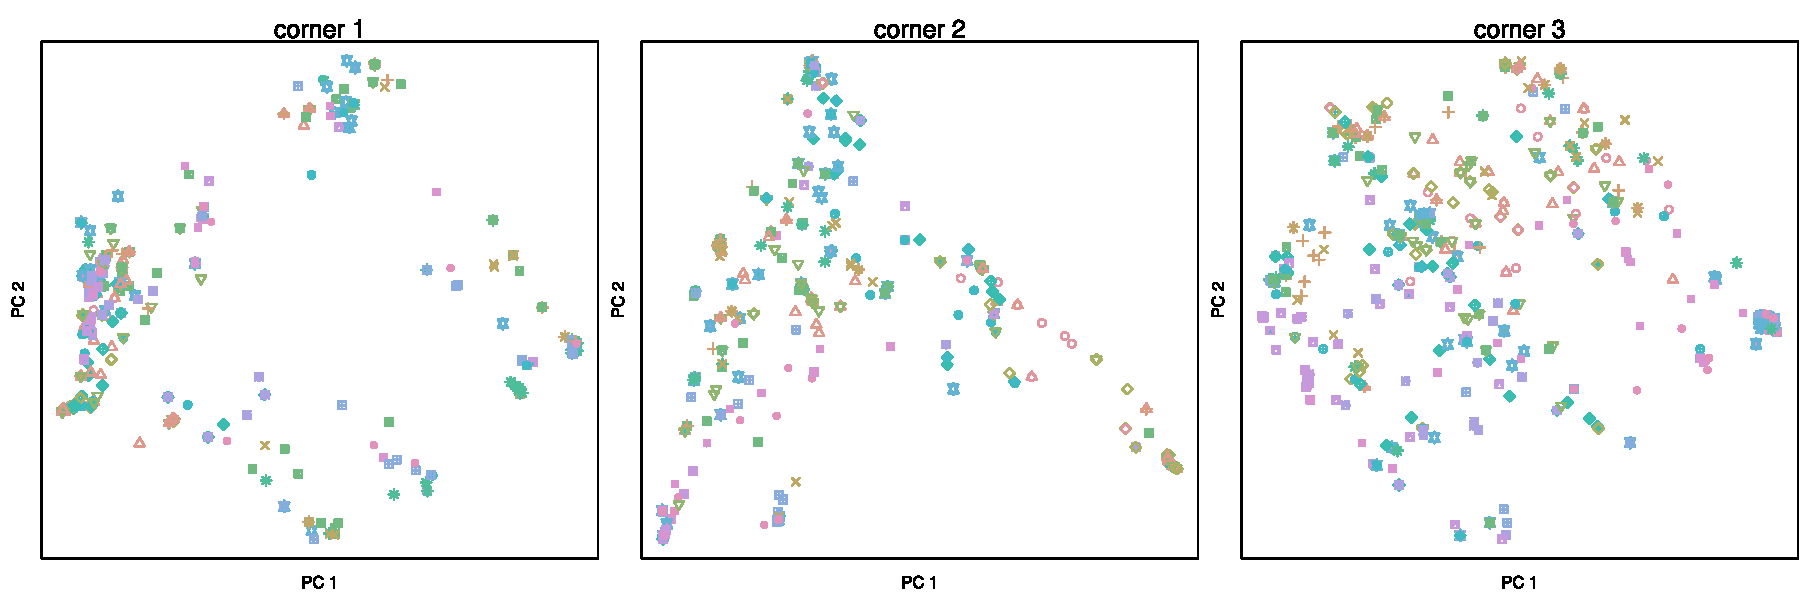
\includegraphics[width=0.82\textwidth]{FigS_plot_corner_pca-1_run_016913}
    \end{center}
    \caption{
        MDS visualizations of the results of individual-based simulations using SLiM
        (see Appendix \ref{apx:slim_sims} for details).
        All simulations incorporate linked selection by allowing selected mutations
        to appear in the same two regions of the genome: 
        the one-sixth of the genome immediately before the halfway point,
        and the last one-sixth of the genome.
        \textbf{(top)} Constant recombination rate.
        \textbf{(top middle)} Stepwise varying recombination rate 
        (as described in \Figure \ref{sfig:slim_sims1}).
        \textbf{(bottom middle)} Constant recombination rate
        with spatially varying effects of selection.
        \textbf{(bottom)} PCA plots corresponding to the highlighted corners 
        of the last MDS visualization, showing how spatially varying linked selection 
        has affected patterns of relatedness.
    } \label{sfig:slim_sims2}
\end{figure}

\begin{figure}
    \begin{center}
        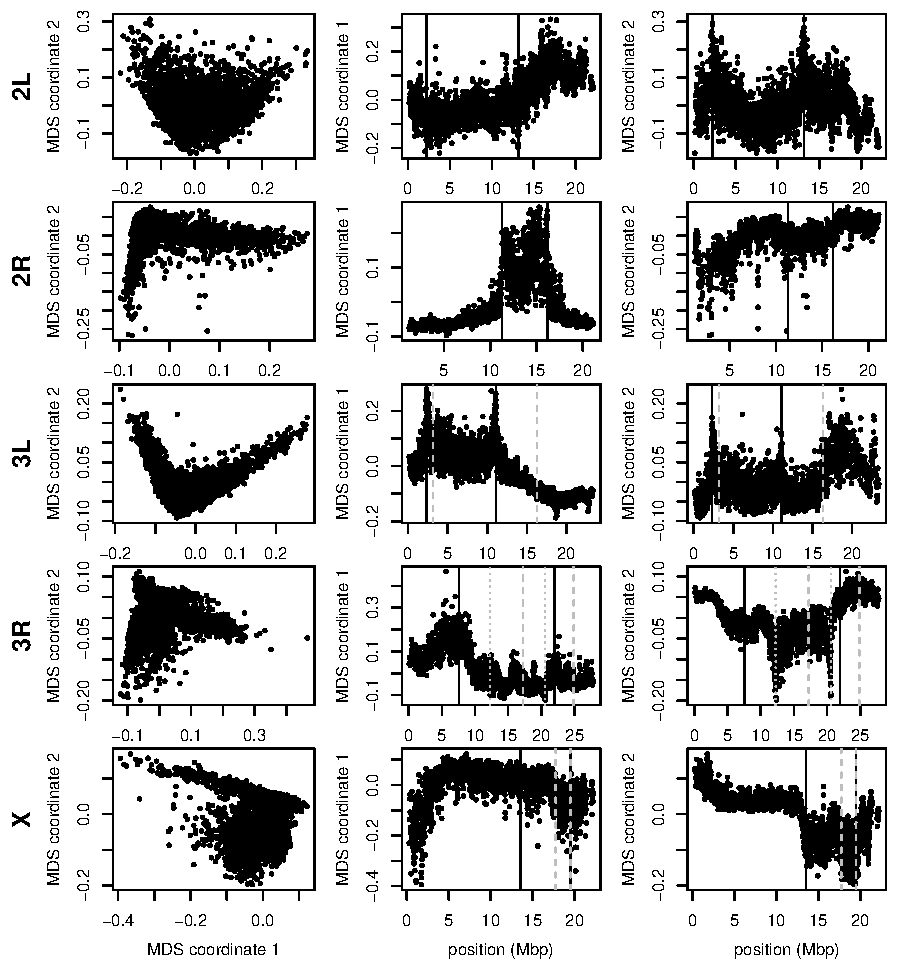
\includegraphics[width=1\textwidth]{Fig1_allchr_Together_MDS_plot_PCAk5_win103}
    \end{center}
    \caption{      
        MDS visualizations for each chromosome arm of \textit{Drosophila melanogaster},
        as in \Figure \ref{fig:mds_allchr},
        except that the method was run using five PCs ($k=5$) instead of two.
         \label{sfig:dmel_k5}
    }
\end{figure}

\begin{figure}
    \begin{center}
       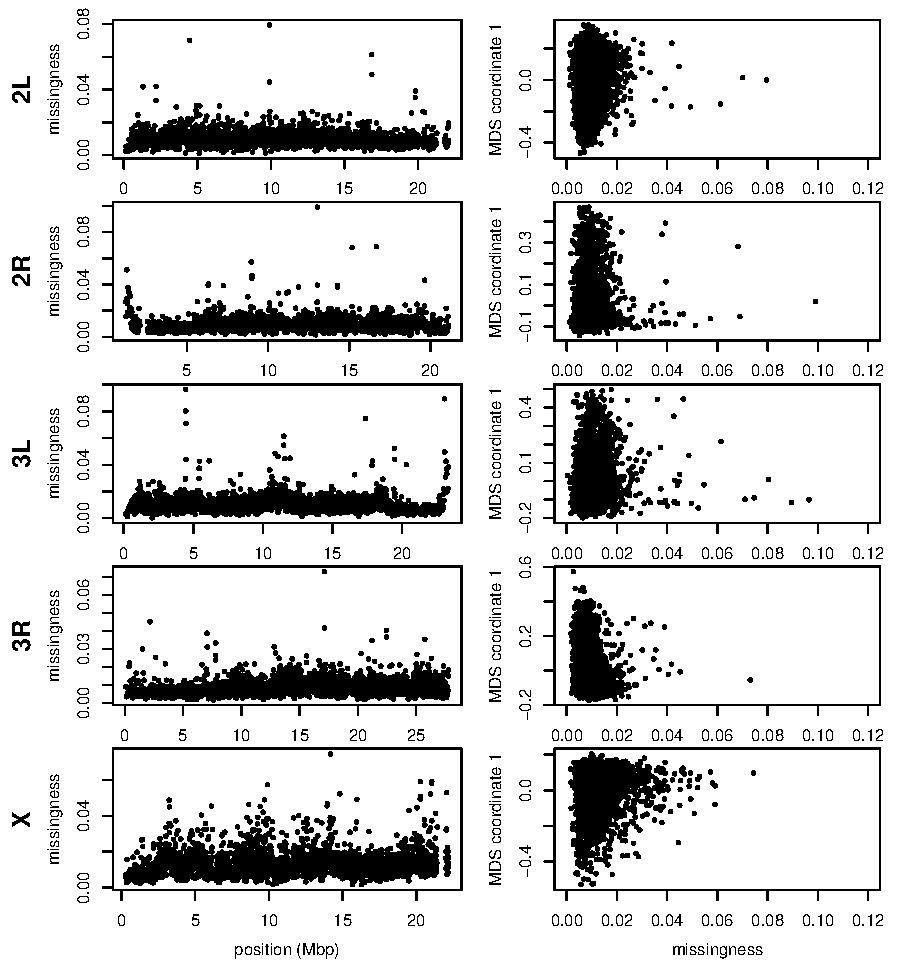
\includegraphics[width=0.82\textwidth]{FigS_Drosophila_missings_against_MDS1_win103}
    \end{center}
    \caption{
        The proportion of data in each window that are missing,
        compared to the value of the first MDS coordinate
        for the \textit{Drosophila melanogaster} data from \Figure \ref{fig:mds_allchr}.
        \label{sfig:dpgp_missingness}
    }
\end{figure}
 
% \begin{figure}
%     \begin{center}
%        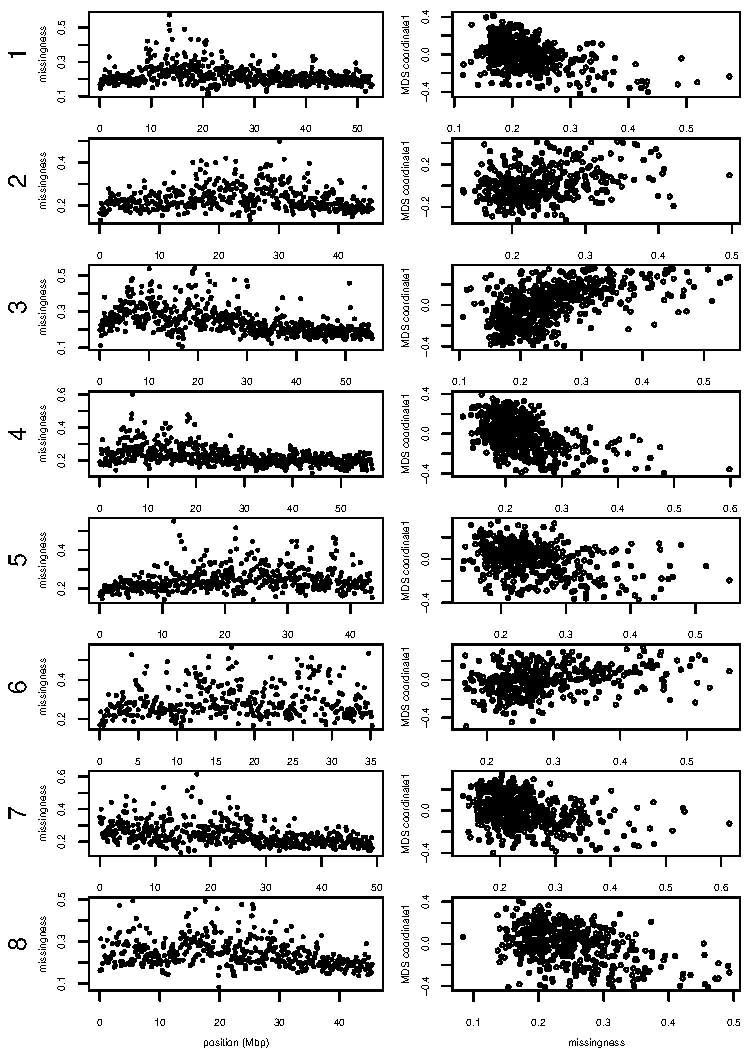
\includegraphics[width=0.82\textwidth]{FigS_Medicago_missing_against_MDS1_win104}
%     \end{center}
%     \caption{
%         The missingness ratio along genome and the correlation of MDS against missingness in Medicago.
%         \label{sfig:medicago_missingness}
%     }
% \end{figure}

\begin{figure}
    \begin{center}
       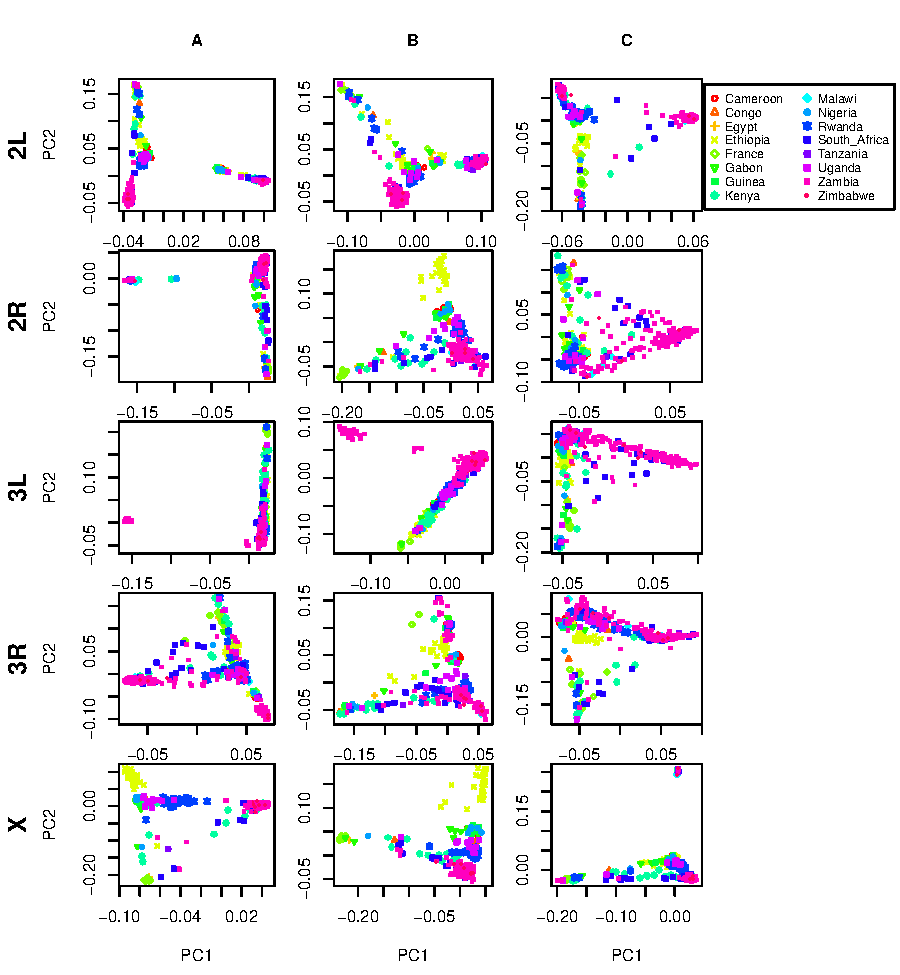
\includegraphics[width=1\textwidth]{Fig2_pca_plots_allchr_3peaks_label_update}
    \end{center}
    \caption{      
        PCA plots for the three sets of genomic windows colored in \Figure \ref{fig:mds_allchr},
        on each chromosome arm of \textit{Drosophila melanogaster}.
        In all plots, each point represents a sample. 
        The first column shows the combined PCA plot for windows 
        whose points are colored green in \Figure \ref{fig:mds_allchr}; 
        the second is for orange windows; 
        and the third is for purple windows.
         \label{sfig:pca_by_pop}
    }
\end{figure}

\begin{figure}
    \begin{center}
        \ifusepngs
            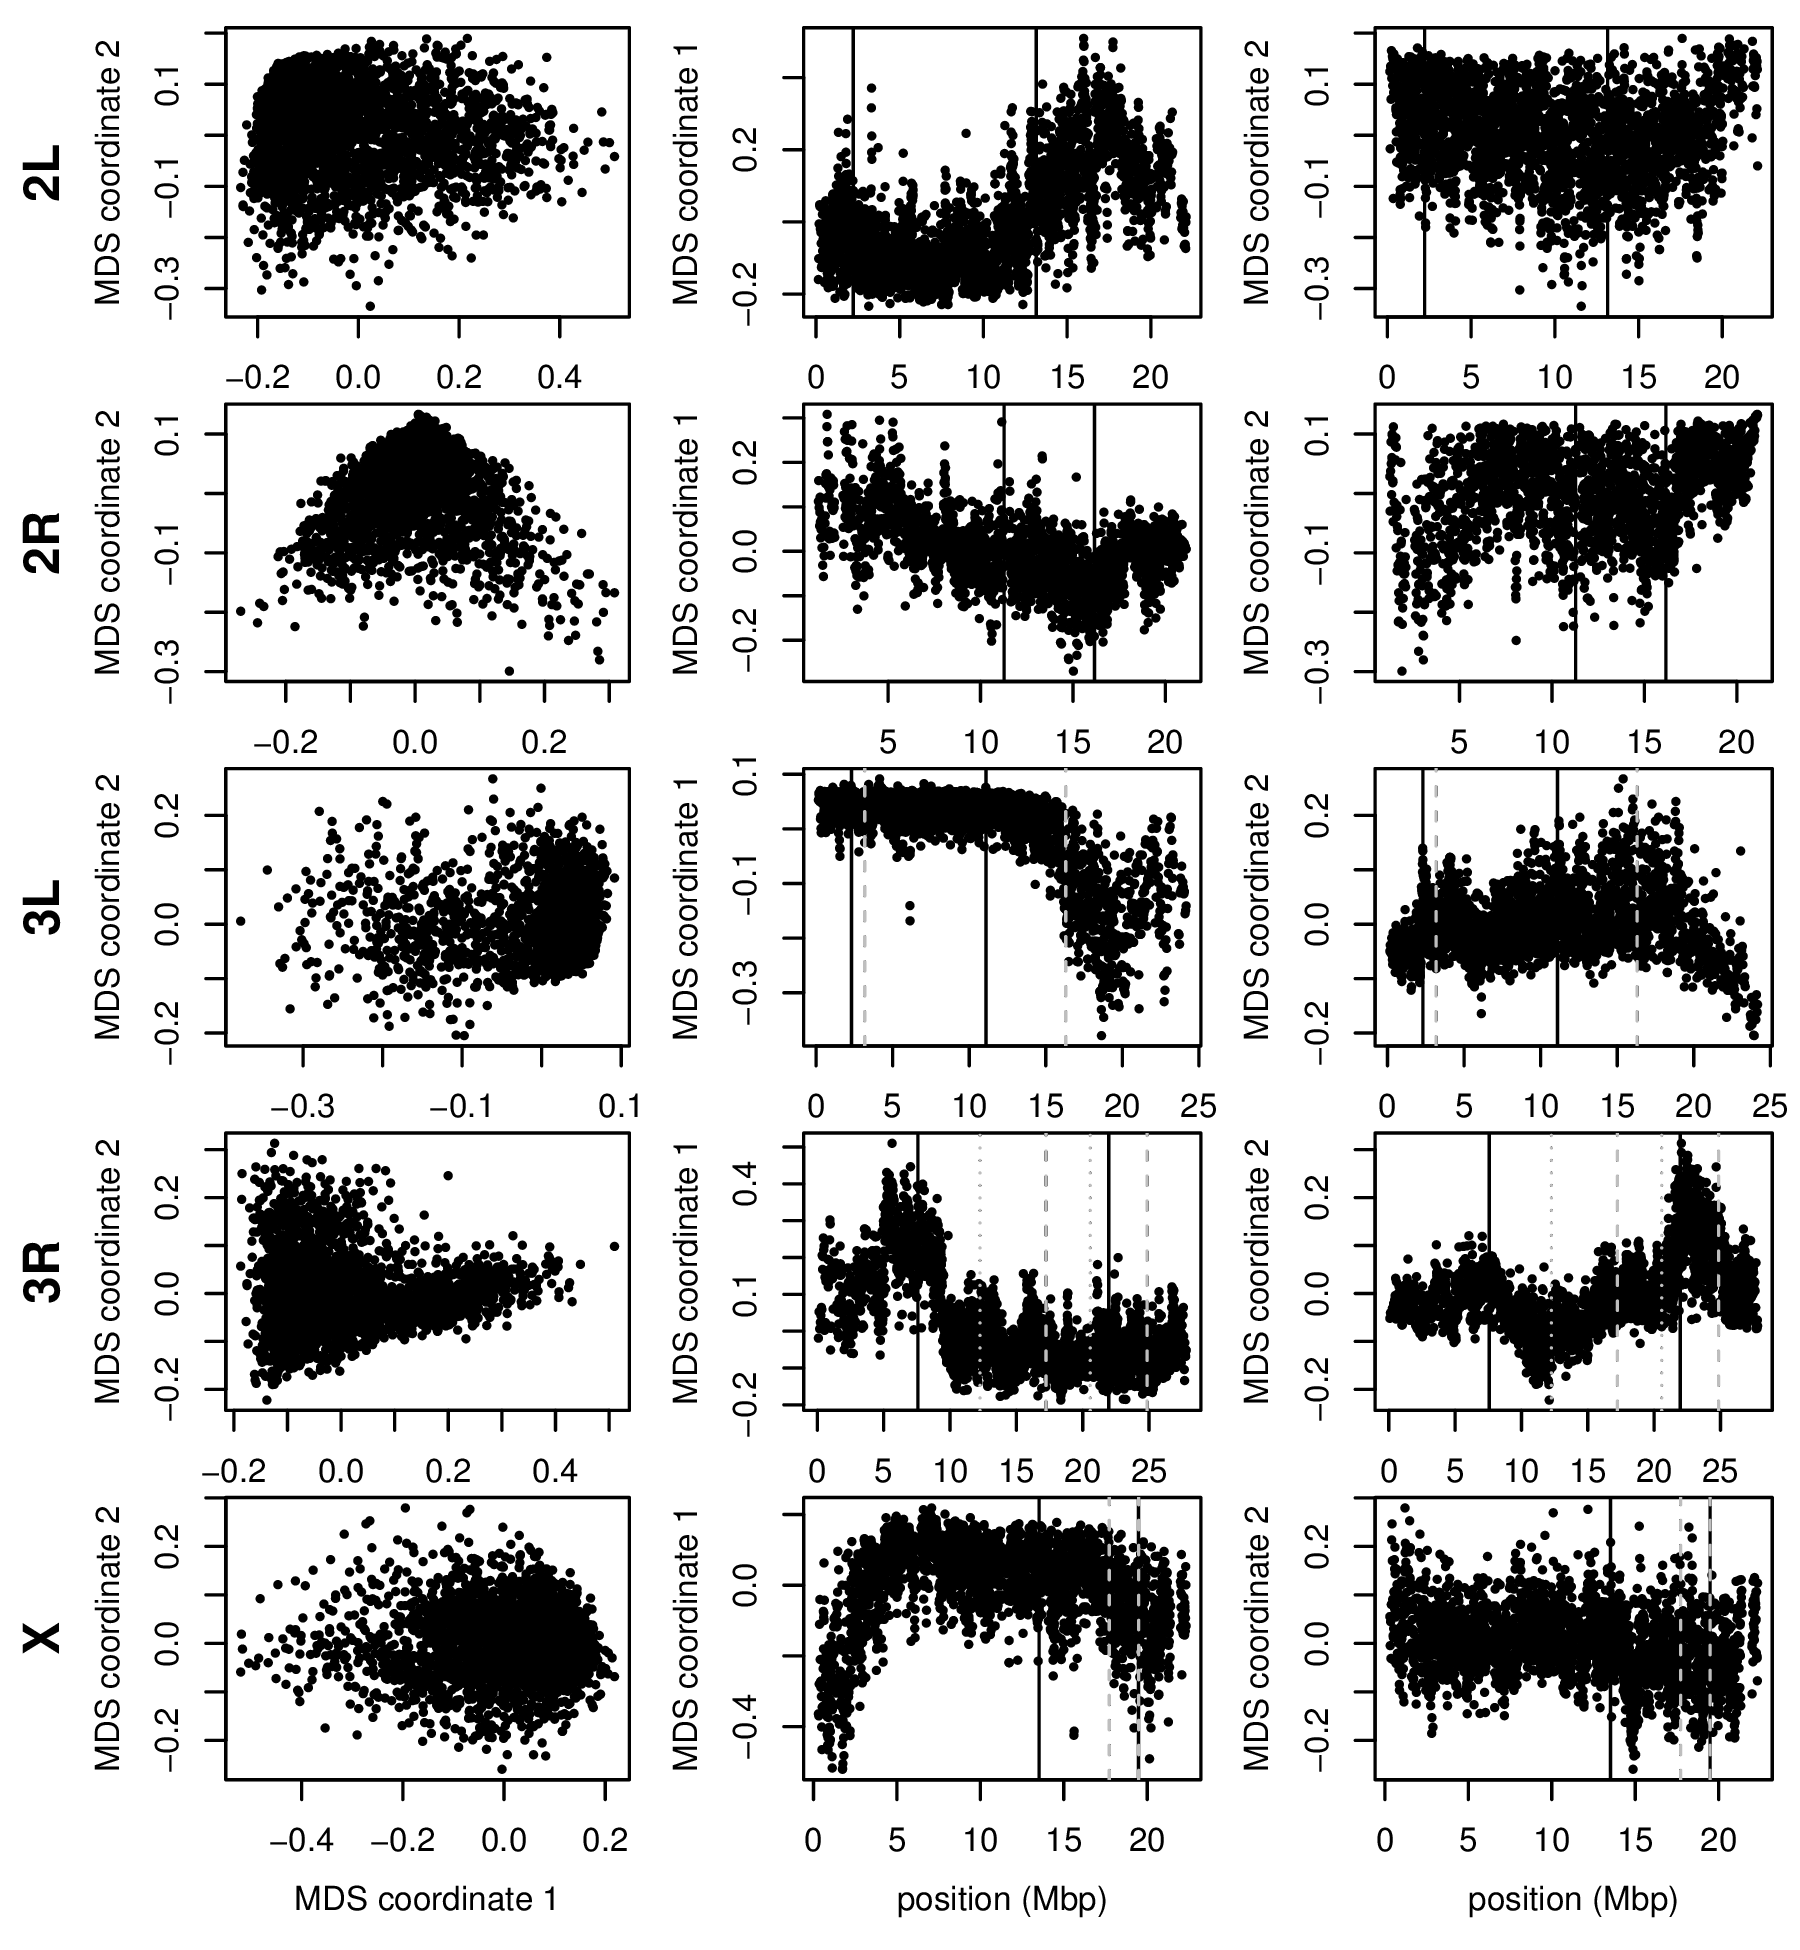
\includegraphics[width=\textwidth]{MDS_allchr_Together_plot_samples_noinv.png}
        \else
            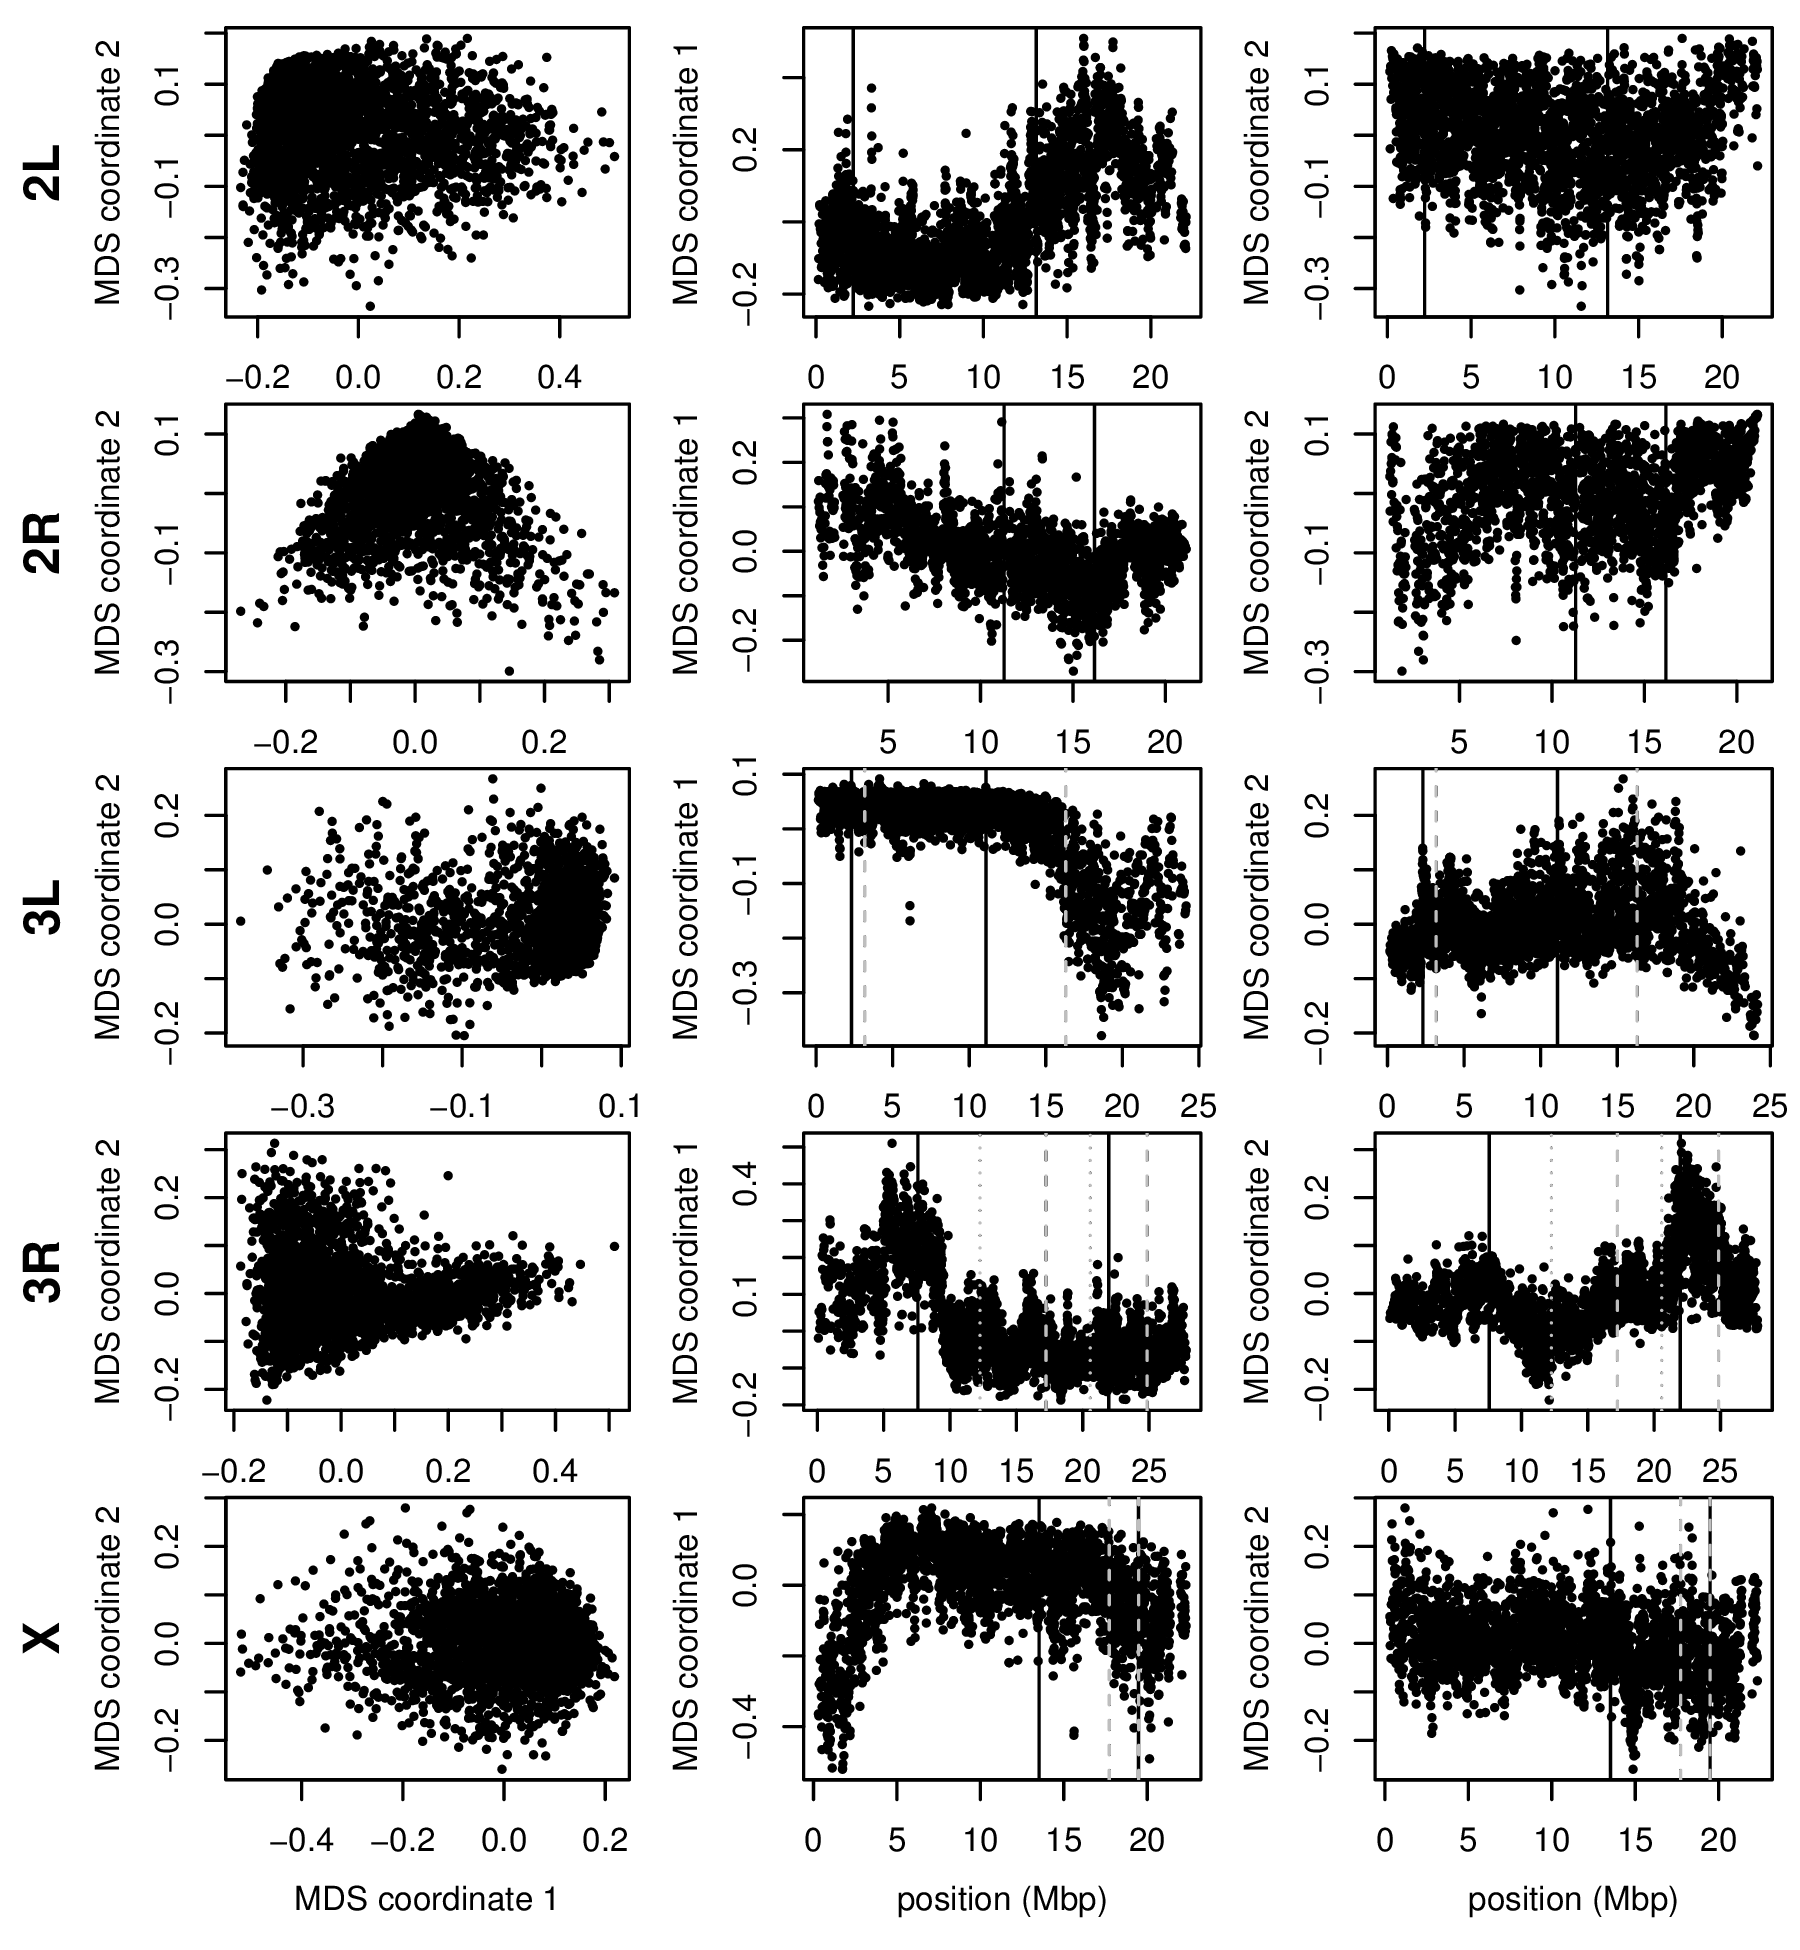
\includegraphics[width=\textwidth]{MDS_allchr_Together_plot_samples_noinv}
        \fi
    \end{center}
    \caption{
        Variation in structure for windows of 1,000 SNPs 
        across \textit{Drosophila melanogaster} chromosome arms: without inversions.
         As in \Figure \ref{fig:mds_allchr}, but after omitting for each chromosome arm individuals carrying the less frequent orientation
         of any inversions on that chromosome arm.
         The values differ from those in \ref{fig:drosophila_recomb_rate}
         in the window size used and that some MDS values were inverted
         (but relative orientation is meaningless as chromosome arms were run separately,
         unlike for \textit{Medicago}).
        In all plots, each point represents one window along the genome.
         The first column shows the MDS visualization of relationships between windows, 
         and the second and third columns show the midpoint of each window against the two MDS coordinates; 
         rows correspond to chromosome arms.
         Vertical lines show the breakpoints of known polymorphic inversions.   
         \label{sfig:mds_allchr_noinversions}
    }
\end{figure}

\begin{figure}
    \begin{center}
        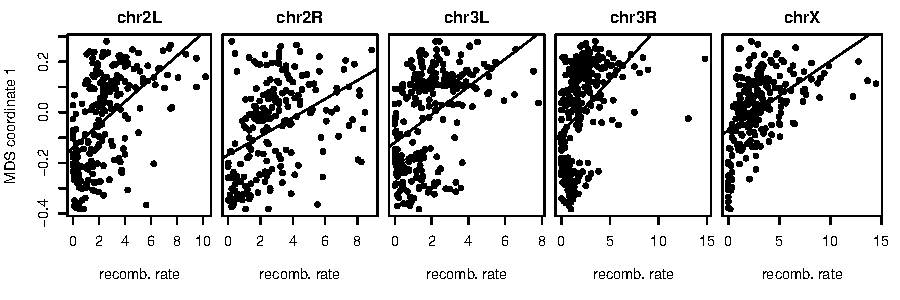
\includegraphics{drosophila_recomb_mds_correlation}
    \end{center}
    \caption{
        Recombination rate, and the effects of population structure for \textit{Drosophila melanogaster}:
        this shows the first MDS coordinate and recombination rate (in cM/Mbp), as in \Figure \ref{fig:drosophila_recomb_rate},
        against each other.
        Since the windows underlying estimates of \Figure \ref{fig:drosophila_recomb_rate} do not coincide,
        to obtain correlations we divided the genome into 100Kbp bins, 
        and for each variable (recombination rate and MDS coordinate 1)
        averaged the values of each overlapping bin with weight proportional to the proportion of overlap.
        The correlation coefficient and $p$-values for each linear regression are as follows:
        2L: correlation $=0.52$, $r^2=0.27$;
        2R: correlation $=0.43$, $r^2=0.18$;
        3L: correlation $=0.47$, $r^2=0.21$;
        3R: correlation $=0.46$, $r^2=0.21$;
        X:  correlation $=0.50$, $r^2=0.24$.
        \label{sfig:drosophila_gene_density_correlations}
    }
\end{figure}


\begin{figure}
    \begin{center}
       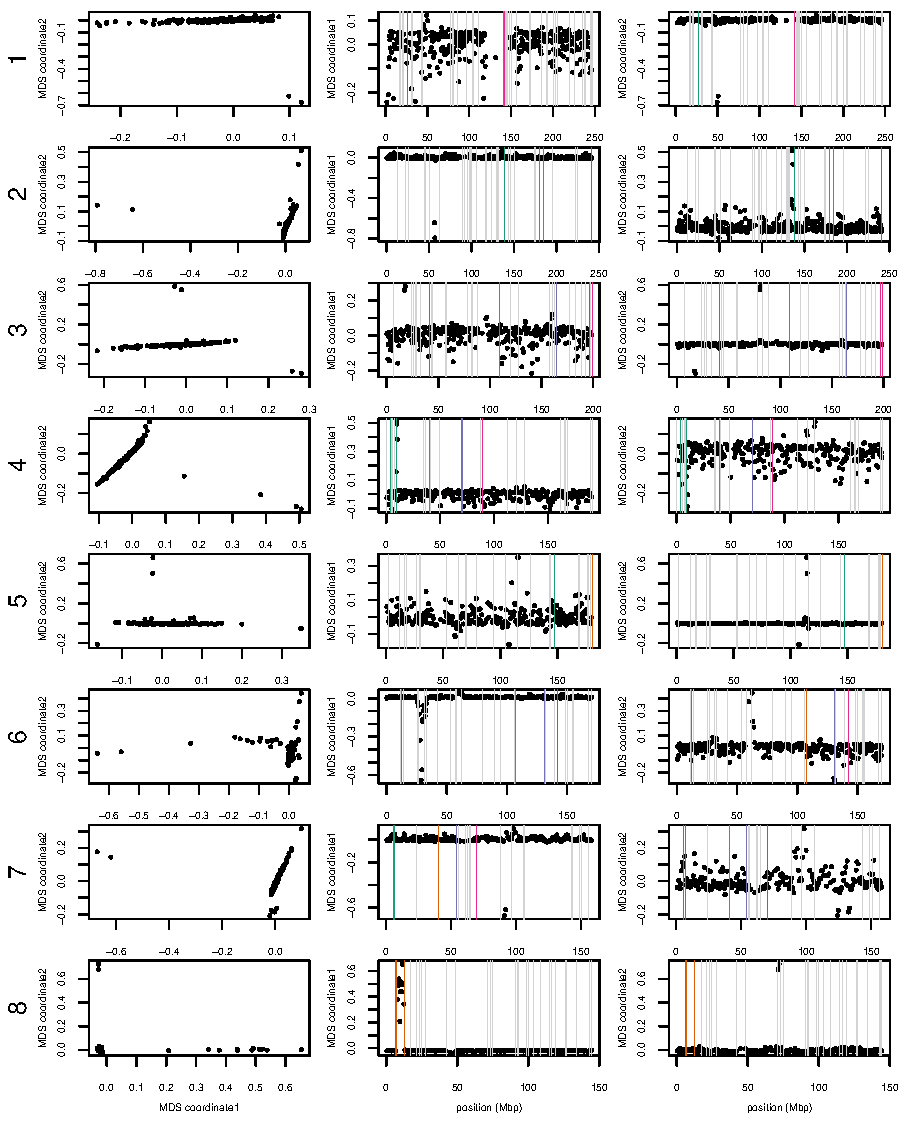
\includegraphics[width=0.9\textwidth]{FigS_human_MDS12_chr1_8_all_valid_and_pre}
    \end{center}
    \caption{
         MDS plots for human chromosomes 1-8.
         The first column shows the MDS visualization of relationships between windows, 
         and the second and third columns show the midpoint of each window against the two MDS coordinates; 
         rows correspond to chromosomes.        
         Colorful vertical lines show the breakpoints of known valid inversions, 
         while grey vertical lines show the breakpoints of predicted inversions.
        \label{sfig:mds12_chr1_8_human}
    }
\end{figure}

\begin{figure}
    \begin{center}
       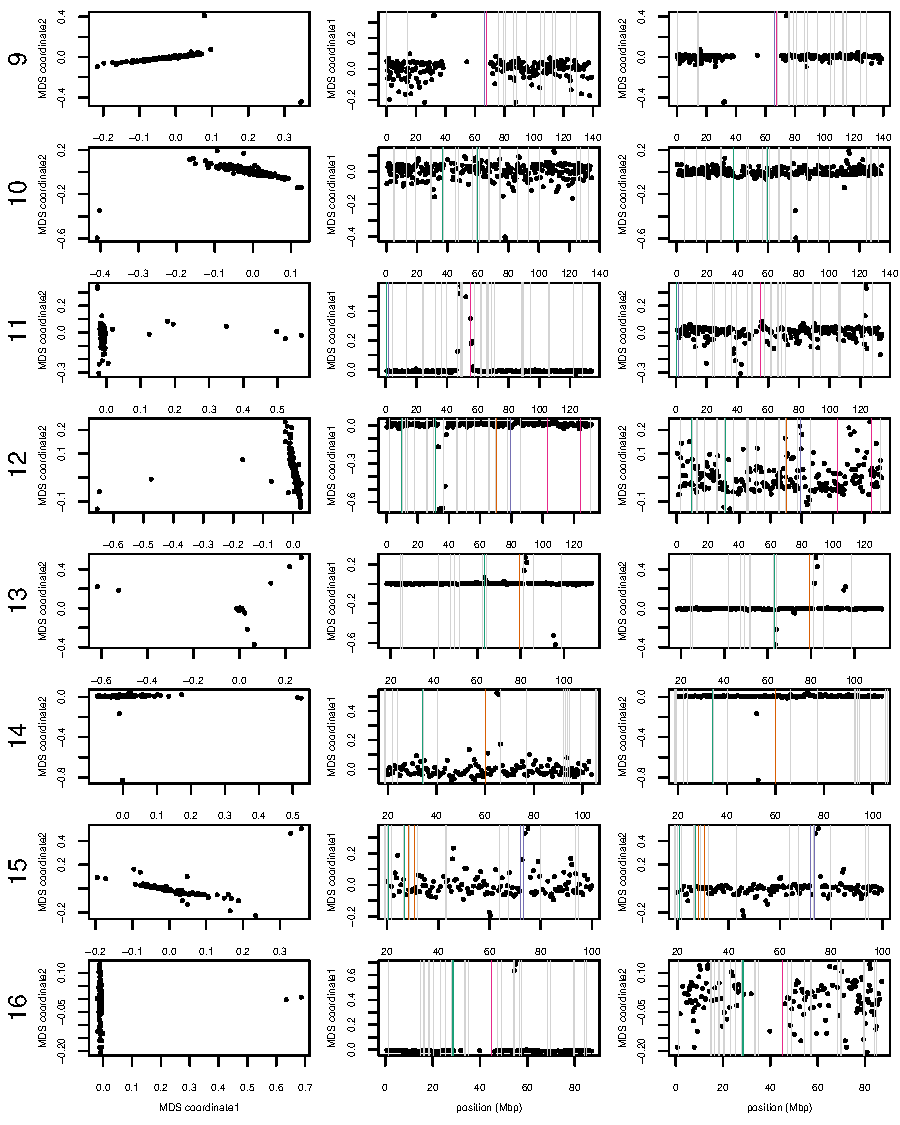
\includegraphics[width=0.9\textwidth]{FigS_human_MDS12_chr9_16_all_valid_and_pre}
    \end{center}
    \caption{
        MDS plots for human chromosomes 9-16, as in Supplemental Figure \ref{sfig:mds12_chr1_8_human}.
        \label{sfig:mds12_chr9_16_human}
    }
\end{figure}

\begin{figure}
    \begin{center}
       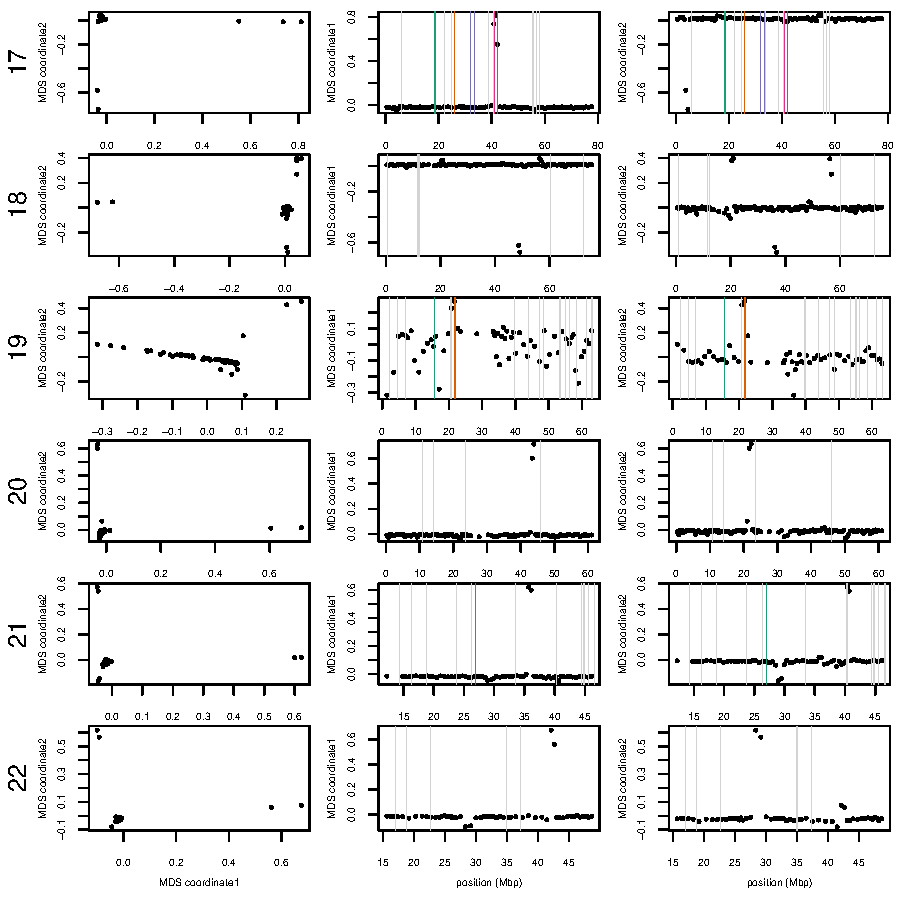
\includegraphics[width=0.9\textwidth]{FigS_human_MDS12_chr17_22_all_valid_and_pre}
    \end{center}
    \caption{
        MDS plots for human chromosomes 17-22, as in Supplemental Figure \ref{sfig:mds12_chr1_8_human}.
        \label{sfig:mds12_chr17_22_human}
    }
\end{figure}

\begin{figure}
    \begin{center}
       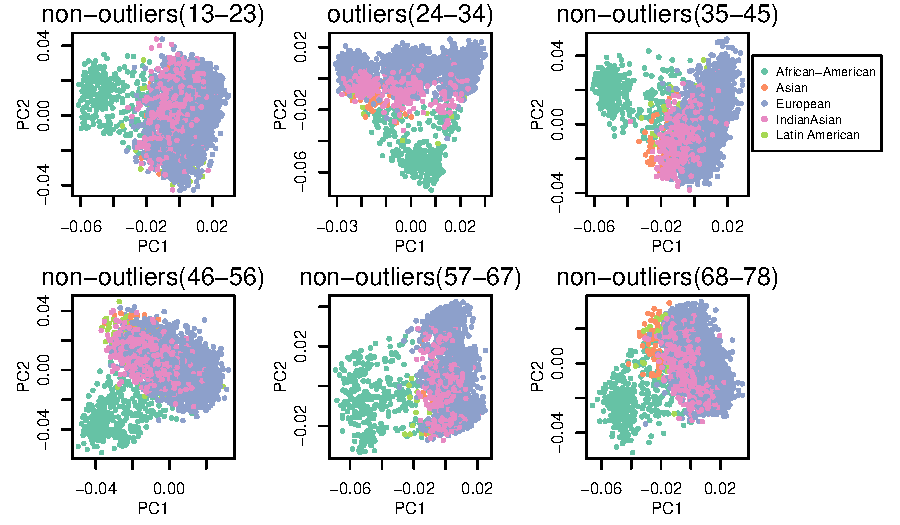
\includegraphics[width=0.9\textwidth]{FigS_PCA_chr8_outliers_combine_update}
    \end{center}
    \caption{
        Comparison of PCA figures within outlying windows (center column)
        and flanking non-outlying windows (left and right columns)
        for the two windows having outlying MDS scores on chromosome 8.
        \label{sfig:pca_chr8_outliers}
    }
\end{figure}

\begin{figure}
    \begin{center}
       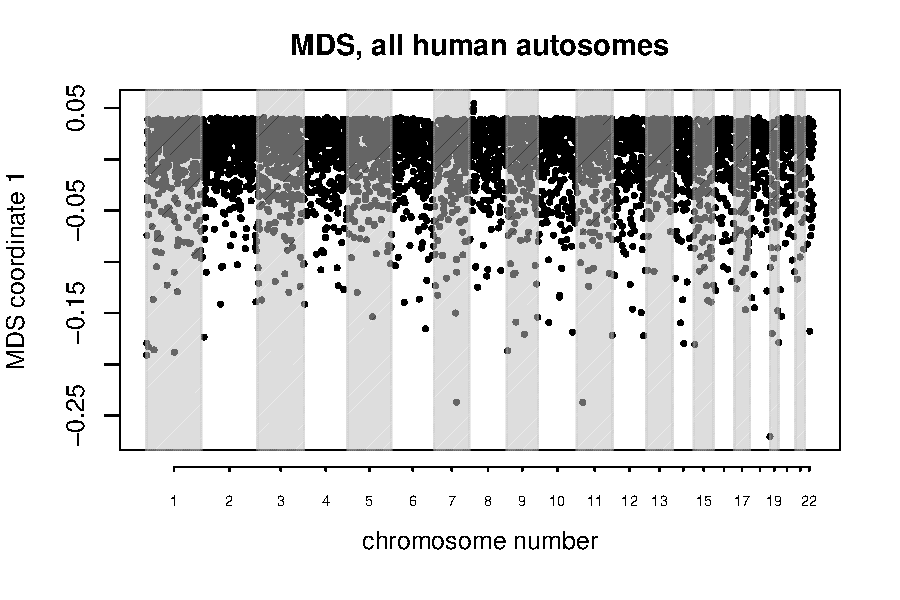
\includegraphics[width=1\textwidth]{FigS_MDS1D_plot_all_chr_human}
    \end{center}
    \caption{
        MDS visualization of variation in the effects of population structure amongst windows across \emph{all} human autosomes simultaneously.
        The small group of windows with positive outlying MDS values lie around the inversion at 8p23.
        \label{sfig:mds1_along_allchr_human}
    }
\end{figure}

\begin{figure}
    \begin{center}
       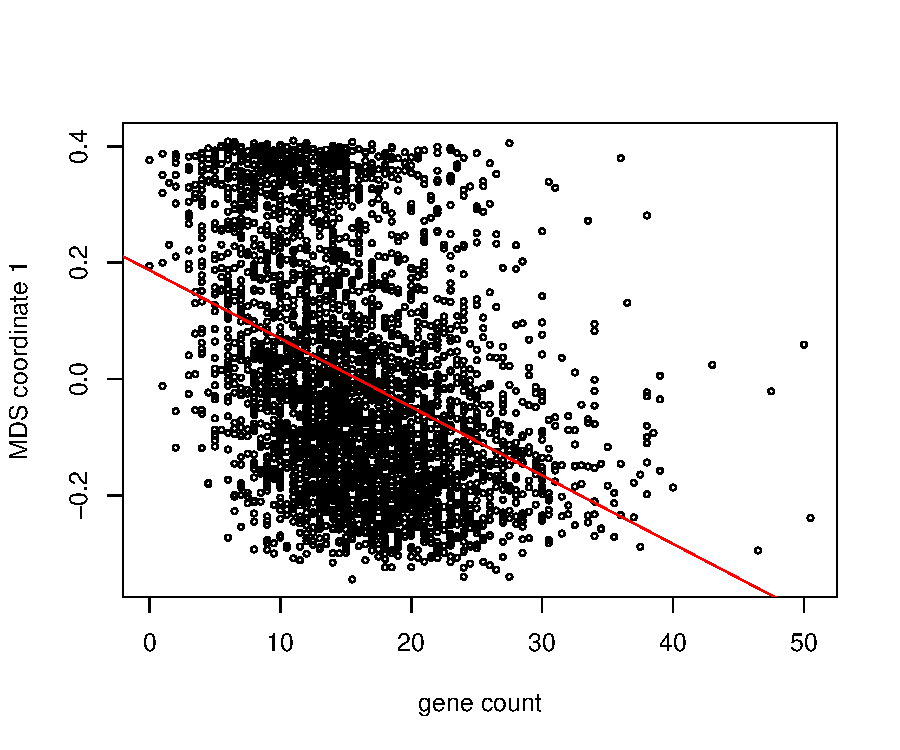
\includegraphics{MDS_1D_against_gene_count_all_chr_win104_with_lm_update}
    \end{center}
    \caption{
        First MDS coordinate against gene density for all 8 chromosomes of \textit{M.~truncatula}.
        The first MDS coordinate is significantly correlated with gene count ($r=0.149$, $p=2.2\times 10^{-16}$). 
        \label{sfig:mds_gene_count}
    }
\end{figure}

% \begin{figure}
%     \begin{center}
%         \ifusepngs
%            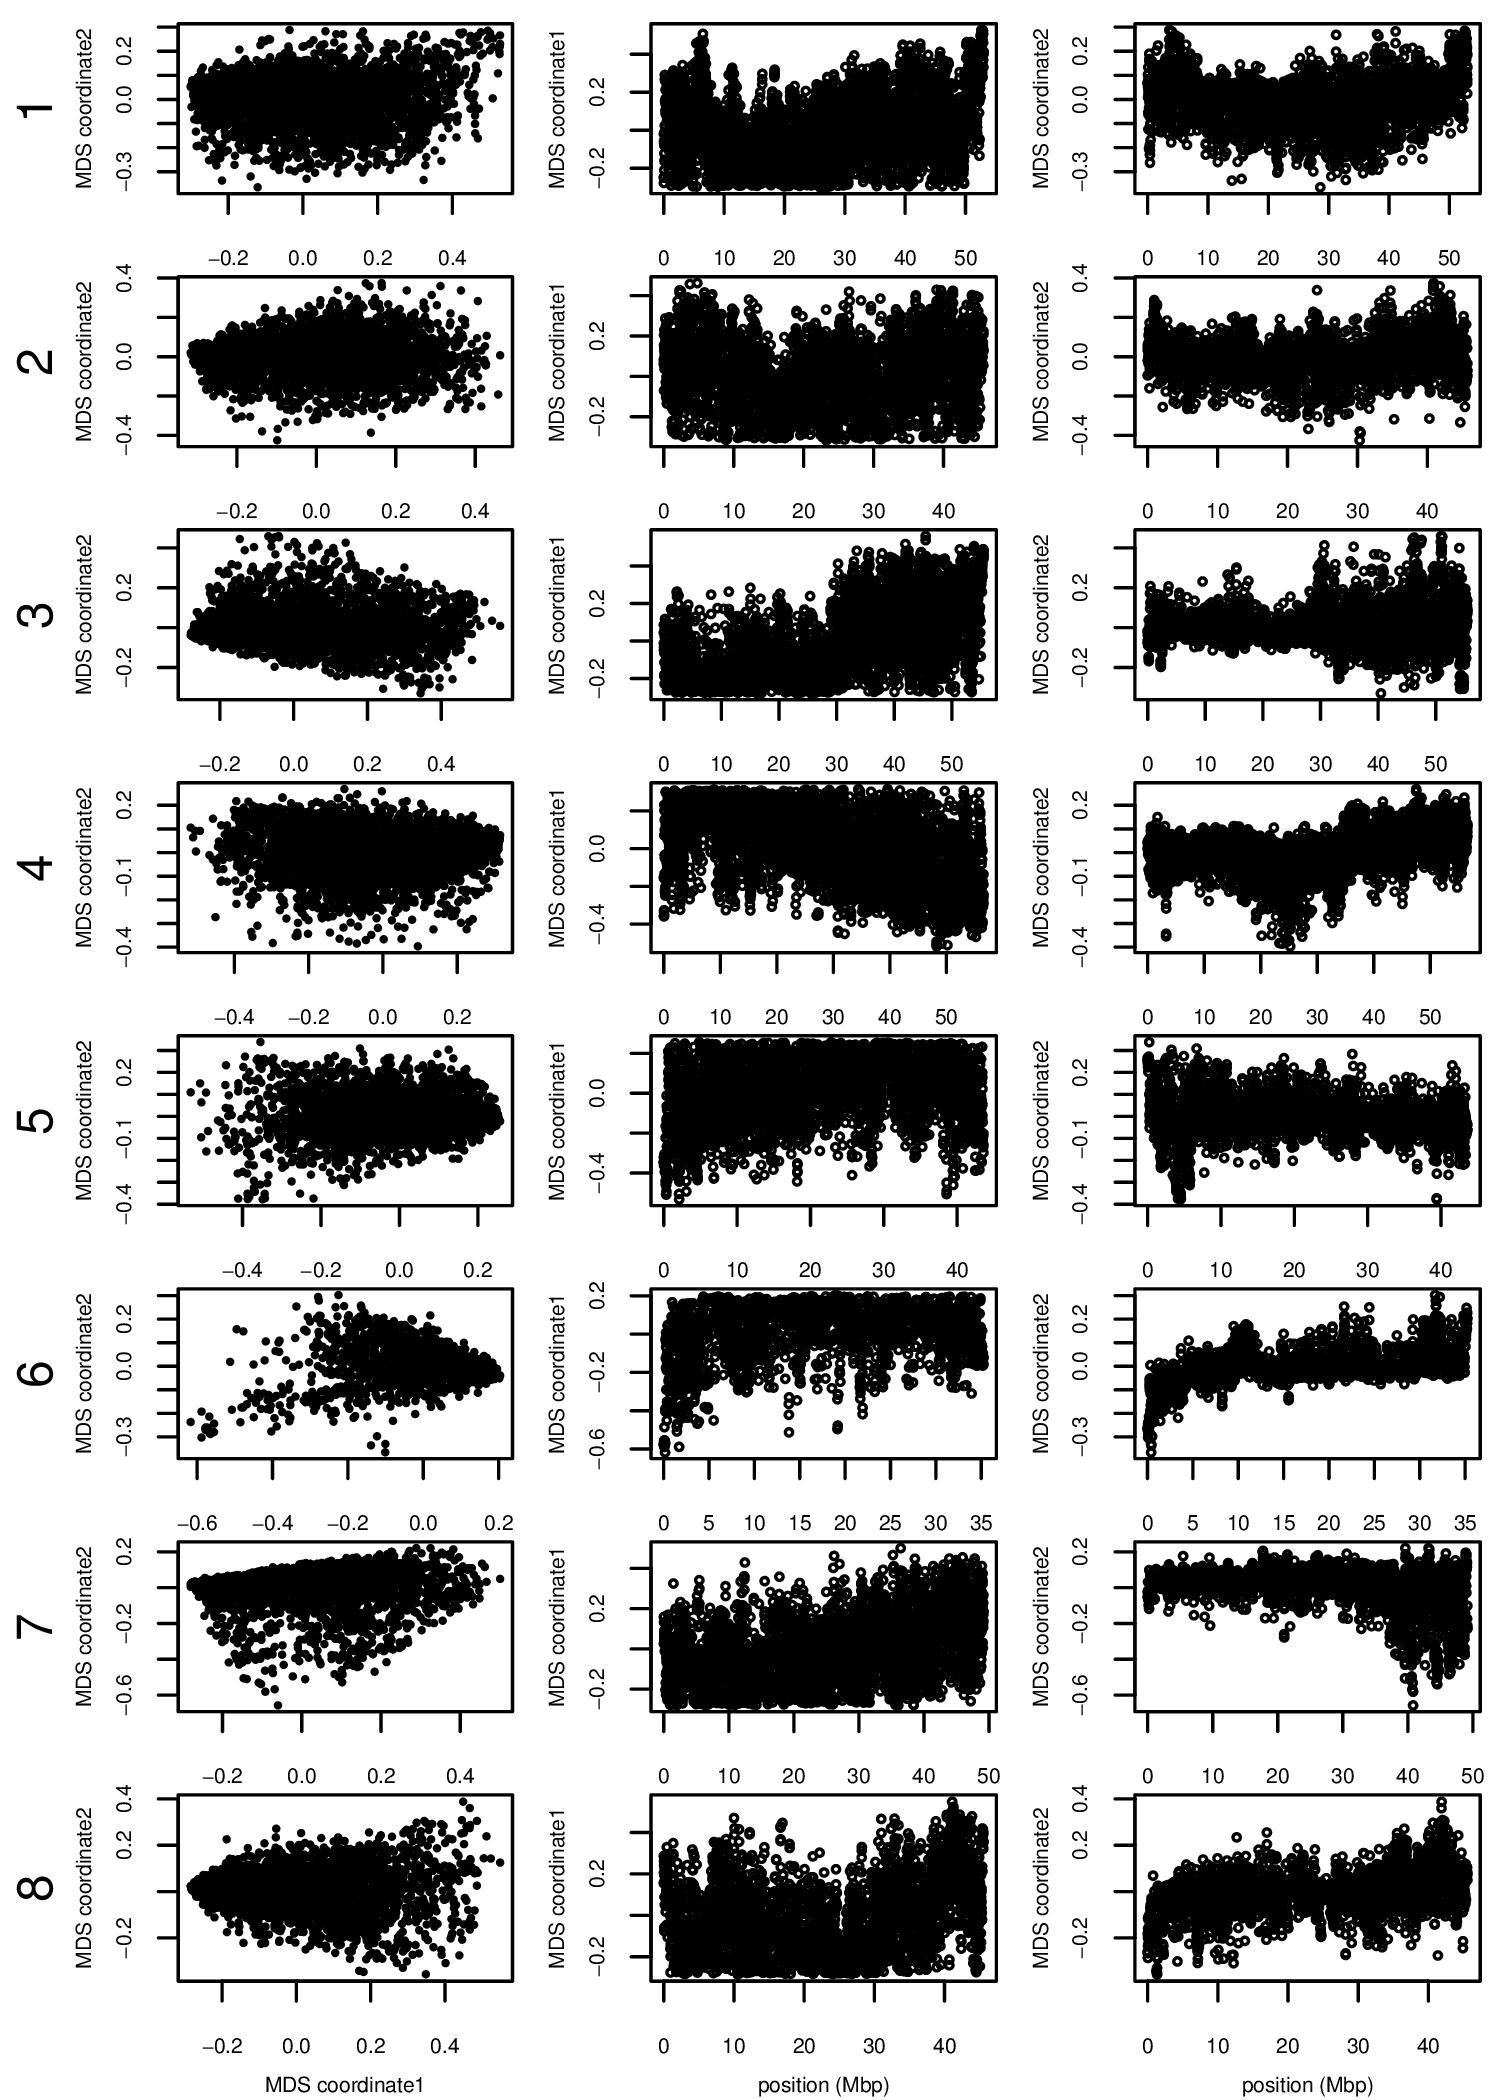
\includegraphics[width=0.85\textwidth]{Medicago_MDS_plot_allchr_win103_PCAk2.png}
%        \else
%            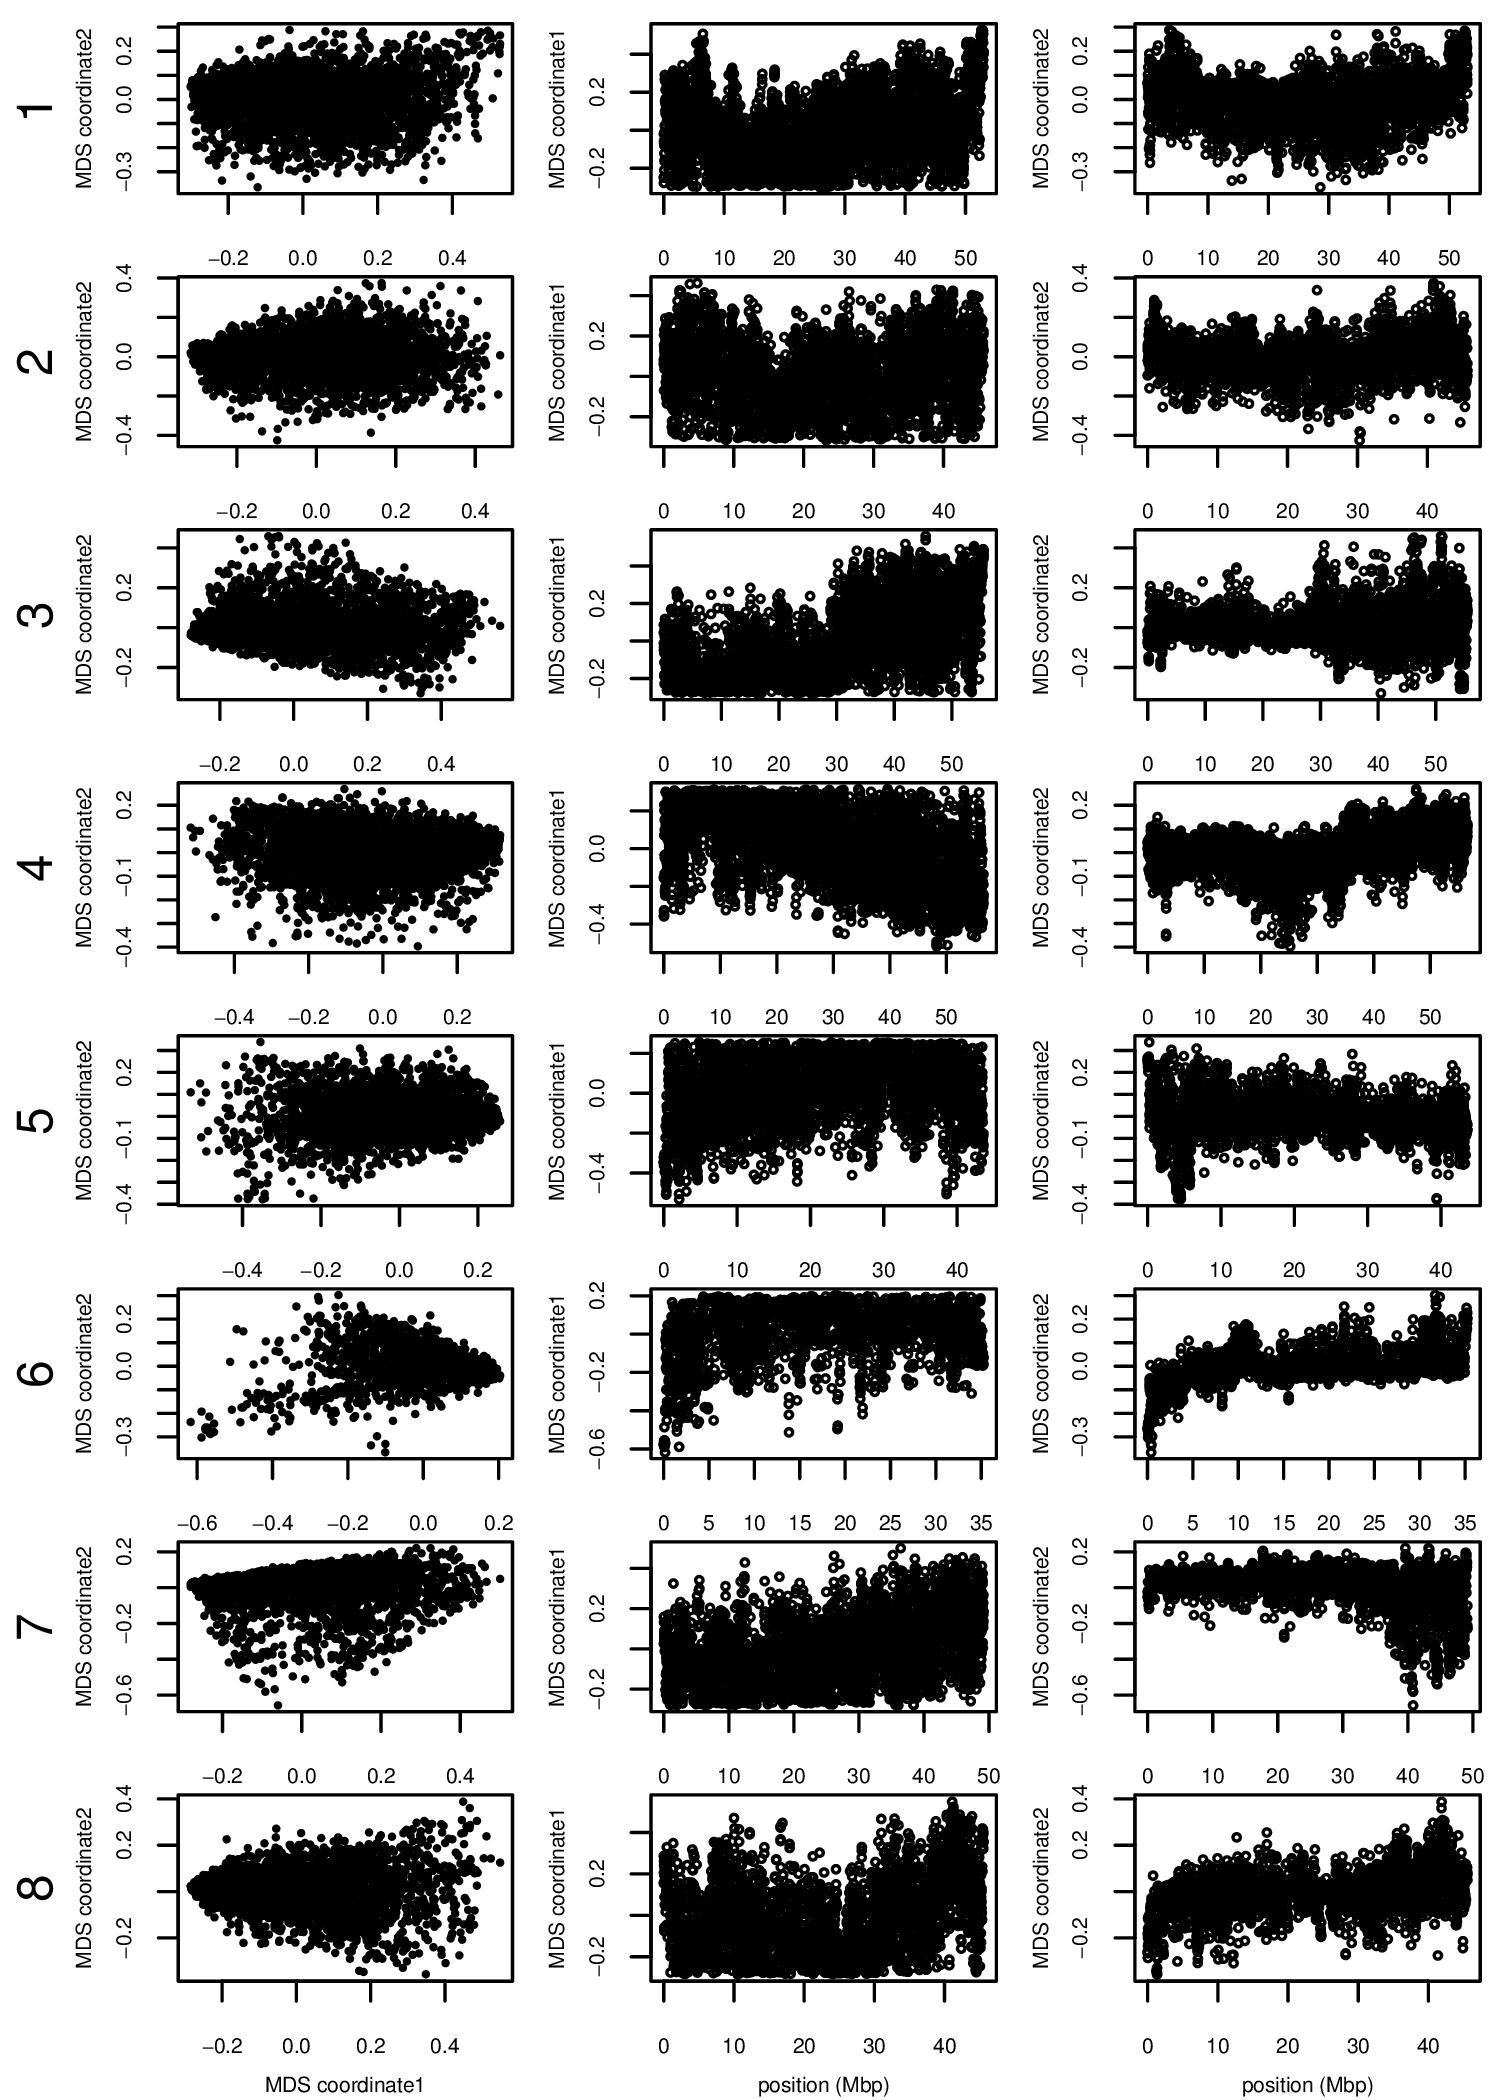
\includegraphics[width=0.85\textwidth]{Medicago_MDS_plot_allchr_win103_PCAk2}
%        \fi
%     \end{center}
%     \caption{
%         MDS visualizations of the effects of population structure for all 8 chromosomes 
%         of the \textit{Medicago truncatula} data as in \Figure \ref{sfig:mds_medicago_allchr},
%         but using windows of $10^3$ SNPs.
%         \label{sfig:mds_medicago_allchr_1e3}
%     }
% \end{figure}

\begin{figure}
    \begin{center}
        \ifusepngs
           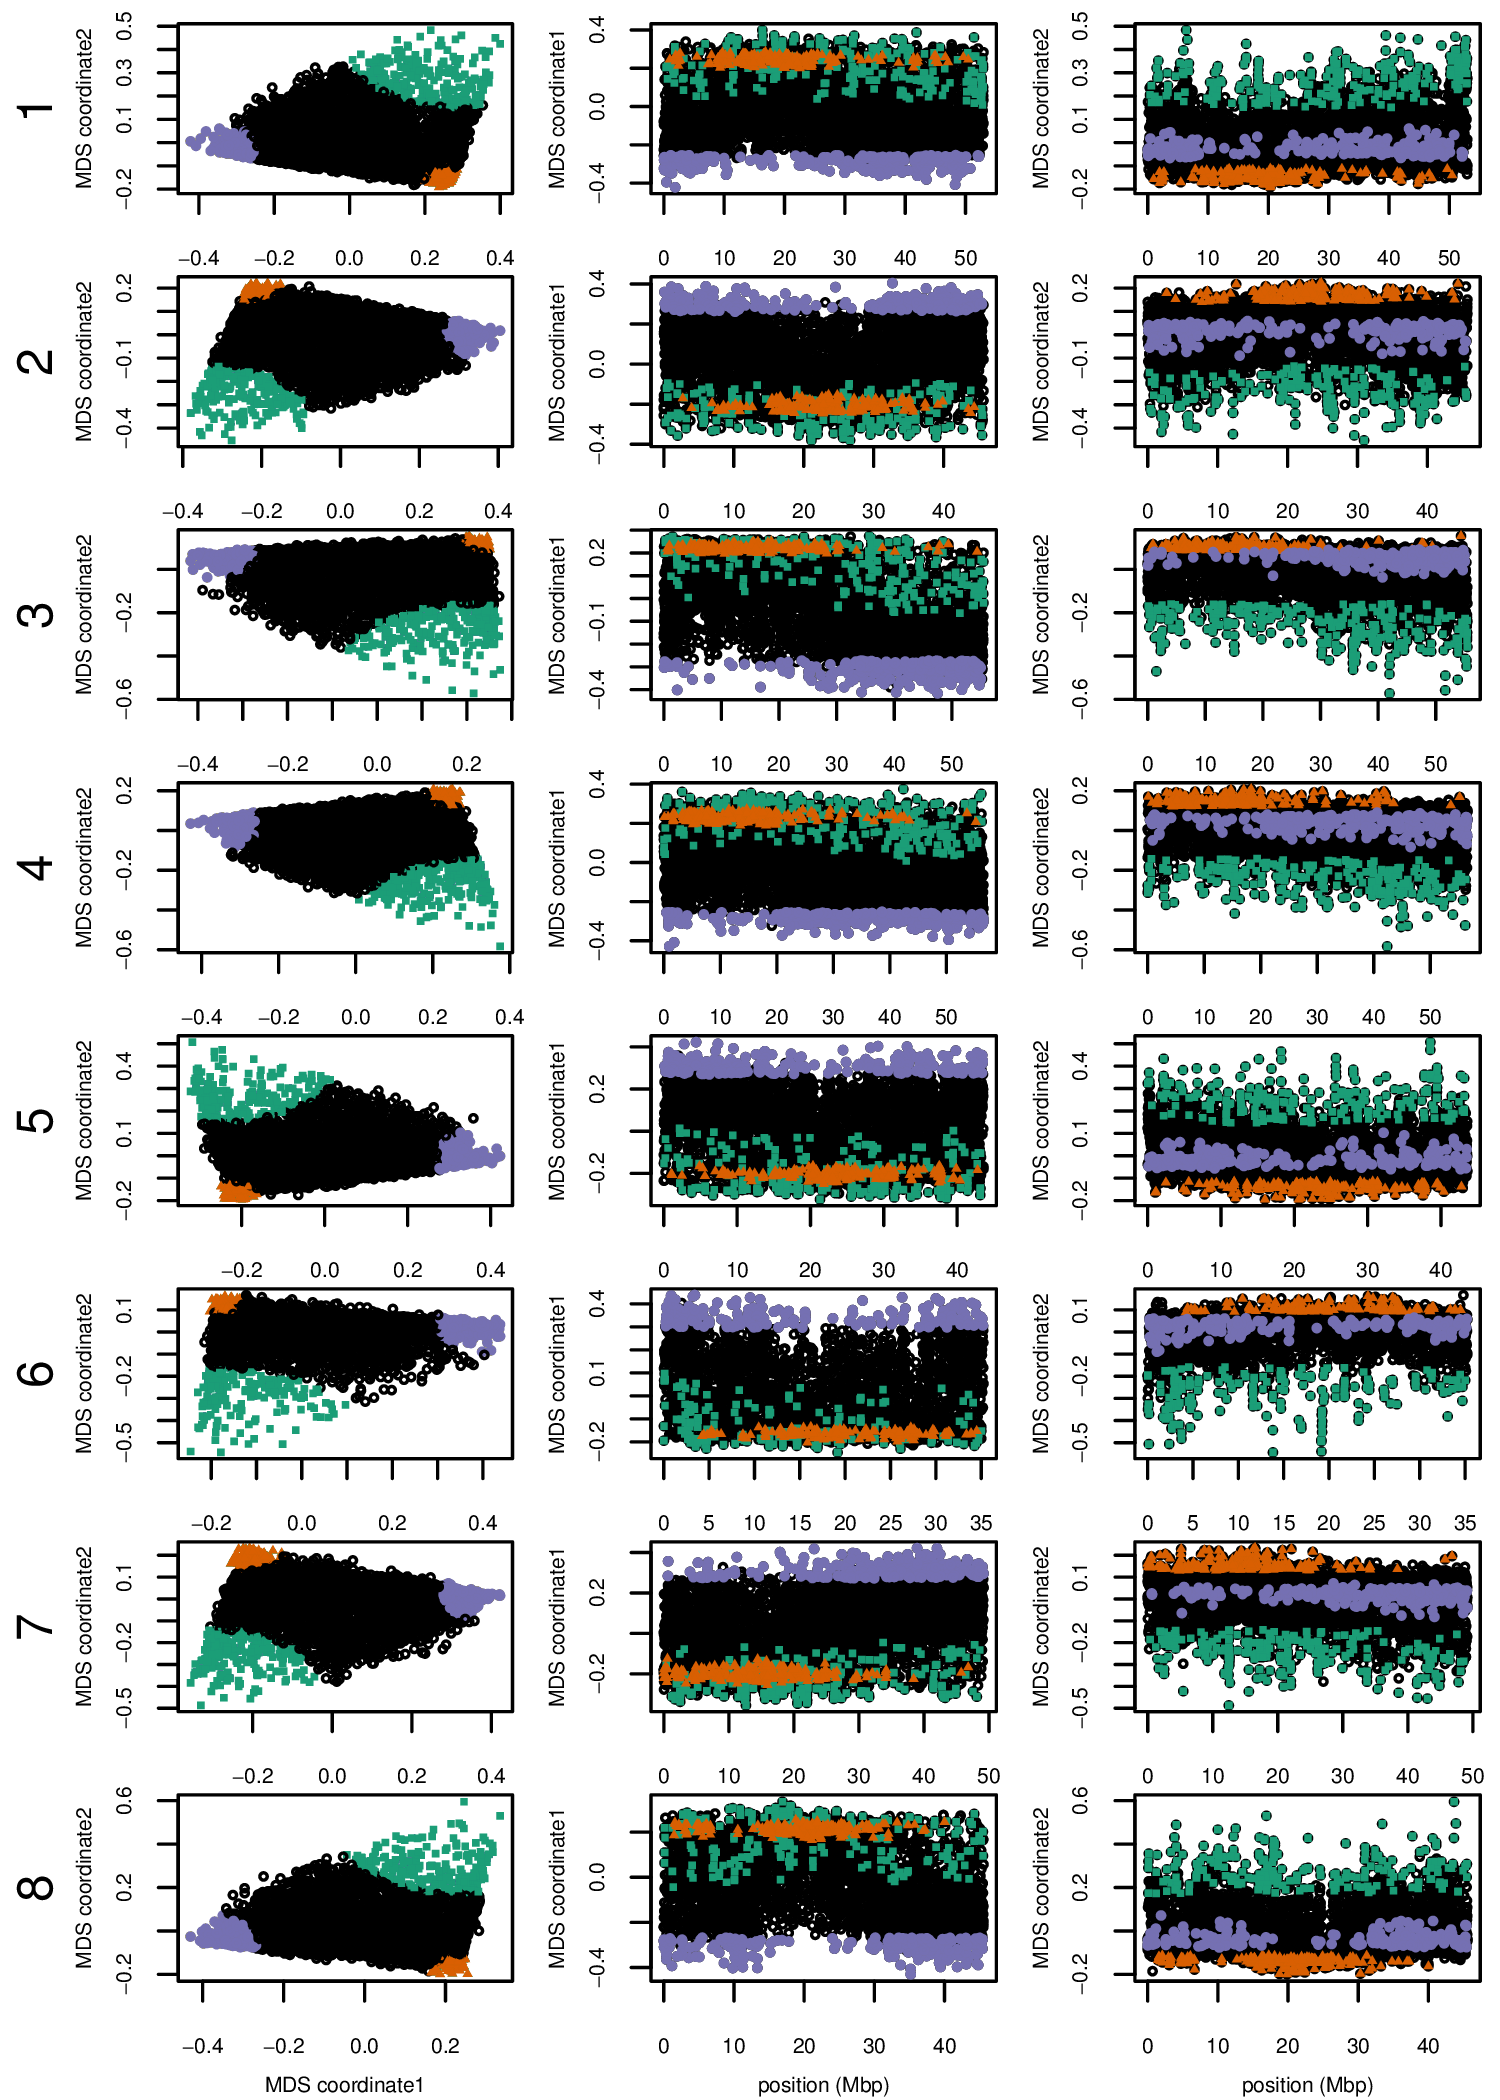
\includegraphics[width=0.85\textwidth]{FigS_Together_MDS_plot_allchr.png}
       \else
           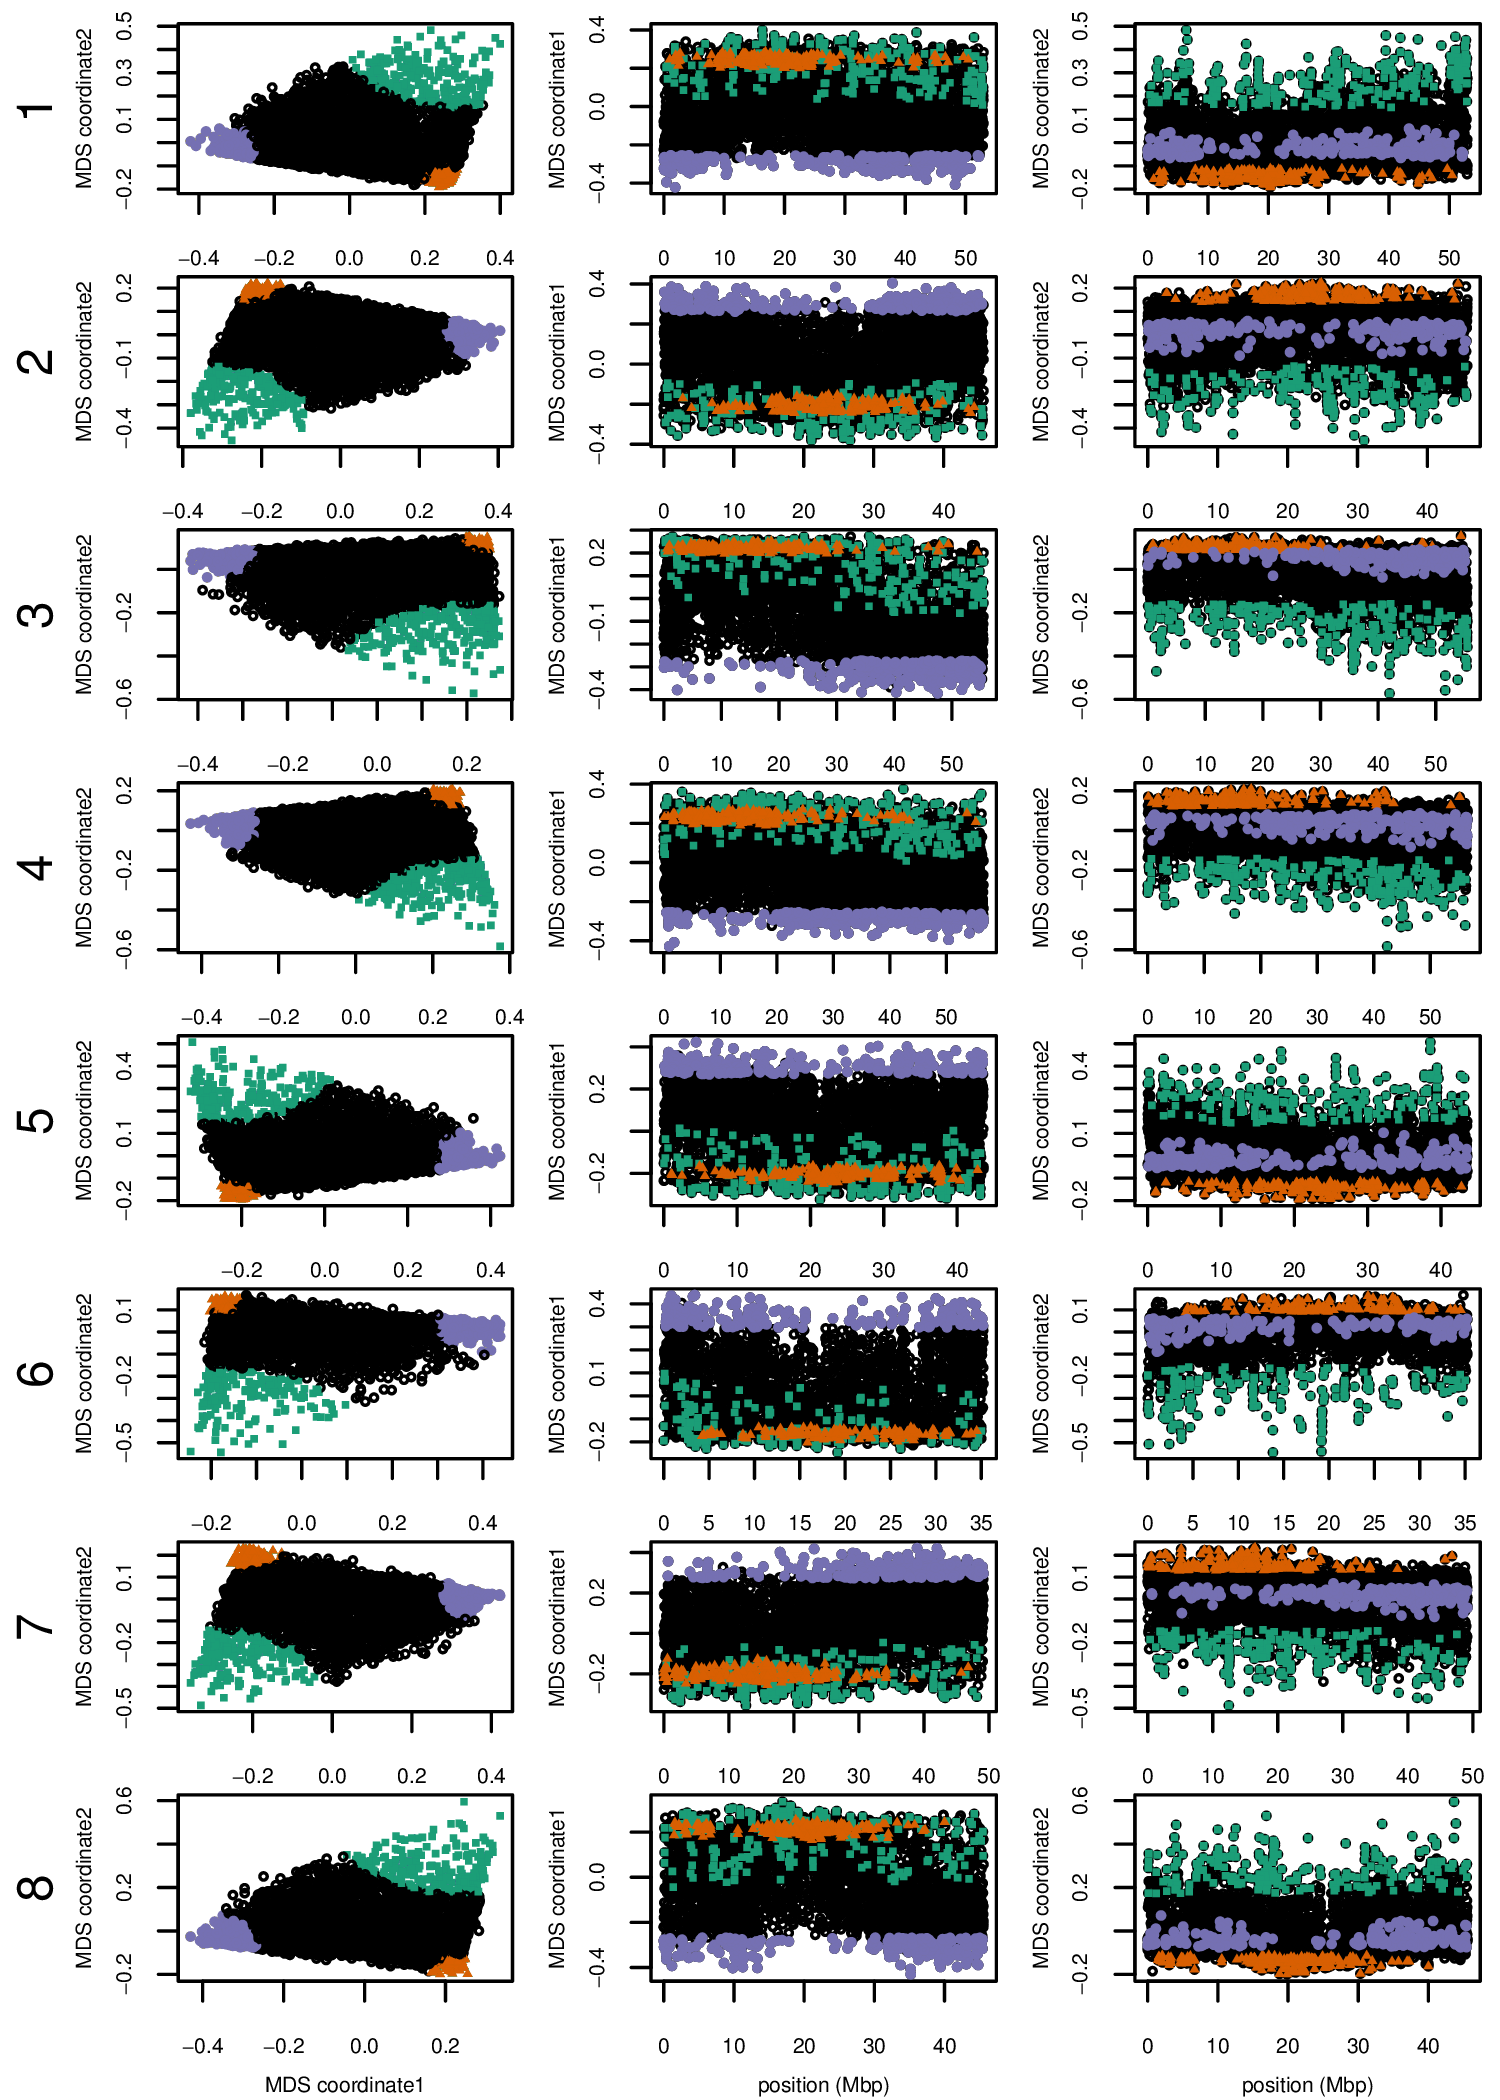
\includegraphics[width=0.85\textwidth]{FigS_Together_MDS_plot_allchr}
       \fi
    \end{center}
    \caption{
        MDS visualizations of the effects of population structure for all 8 chromosomes 
        of the \textit{Medicago truncatula} data, using windows of $10^4$ SNPs.
        \label{sfig:mds_medicago_allchr}
    }
\end{figure}



\begin{figure}
    \begin{center}
       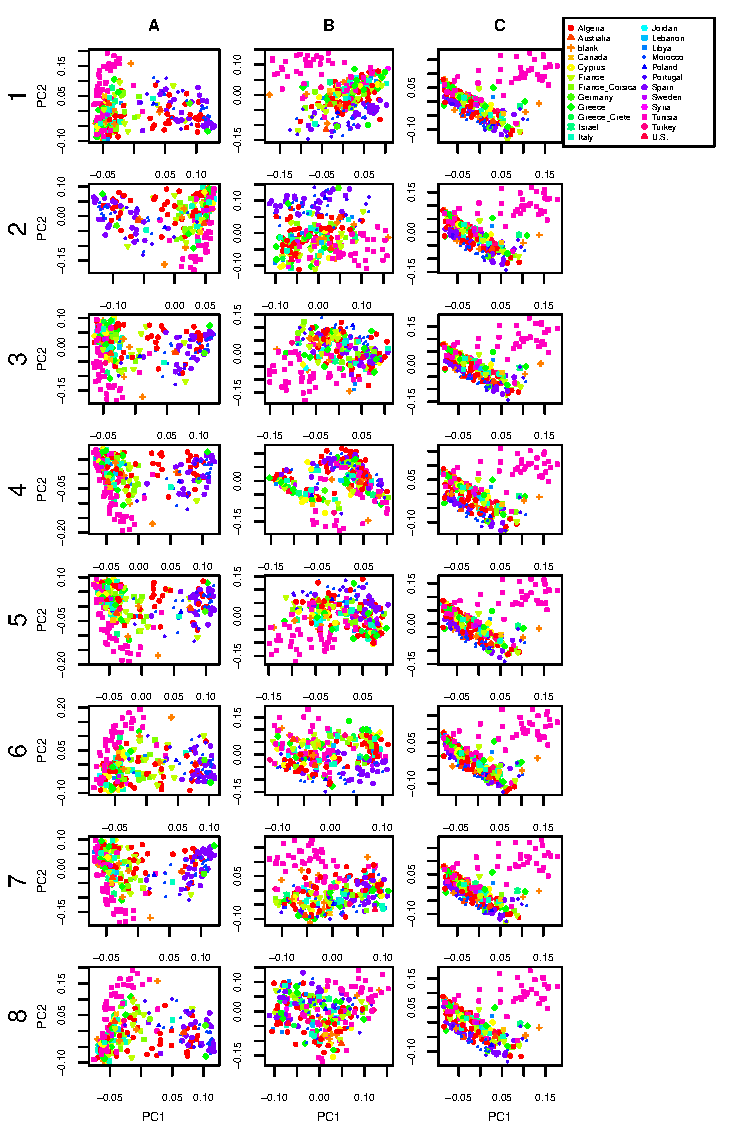
\includegraphics[width=0.82\textwidth]{FigS_pca_plots_for_Medicago_allchr_3peaks_byMDS}
    \end{center}
    \caption{
        PCA plots for regions colored in \Figure \ref{sfig:mds_medicago_allchr}
        on all 8 chromosomes of \textit{Medicago truncatula}:
        (A) green, (B) orange, and (C) purple.
        \label{sfig:pca_peaks_medicago_allchr}
    }
\end{figure}







\ifsubmission\processdelayedfloats\fi

% reviews here if toggled above
\includereviews


\end{document}  
